  \documentclass[11pt]{article}
\usepackage{fullpage}
\usepackage[utf8]{inputenc}
\usepackage[T1]{fontenc}
\usepackage{empheq}
\usepackage{color}
\usepackage {listings}
\usepackage{amsmath}
\usepackage{hyperref}
\usepackage{longtable}
\usepackage{array}
%\usepackage[scaled]{beramono}
\usepackage[T1]{fontenc}
\usepackage{tabularx}
\usepackage{amssymb}
\usepackage{enumitem}
\usepackage{booktabs}
\usepackage{multirow} 
\usepackage{tipa}

%\setmonofont{Consolas} %to be used with XeLaTeX or LuaLaTeX
\definecolor{bluekeywords}{rgb}{0,0,1}
\definecolor{blue(munsell)}{rgb}{0.0, 0.5, 0.69}
\definecolor{greencomments}{rgb}{0,0.5,0}
\definecolor{redstrings}{rgb}{0.64,0.08,0.08}
\definecolor{xmlcomments}{rgb}{0.5,0.5,0.5}
\definecolor{types}{rgb}{0.17,0.57,0.68}
\setlength\parindent{0pt}

\lstset{language=[Sharp]C,
captionpos=b,
%numbers=left, %Nummerierung
%numberstyle=\tiny, % kleine Zeilennummern
frame=lines, % Oberhalb und unterhalb des Listings ist eine Linie
showspaces=false,
showtabs=false,
breaklines=true,
showstringspaces=false,
breakatwhitespace=true,
escapeinside={(*@}{@*)},
commentstyle=\color{greencomments},
morekeywords={partial, var, get, set,string,false,true},
keywordstyle=\color{bluekeywords},
stringstyle=\color{redstrings},
basicstyle=\ttfamily\small,
extendedchars=true,
literate={à}{{\`a}}1 {è}{{\`e}}1 {ò}{{\`o}}1 {ù}{{\`u}}1 {é}{{\'e}}1,
}
\lstset%
{%
    emph=[1]%
    {%
        Process,
        Cplex,
        Program,
        IntParam,
        NumVarType,
        INumVar,
        SystemInformation,
        Param,
        Stopwatch,
        Instance,
        ProcessStartInfo,
        Point,
        ILinearNumExpr,
        List,
        PathGenetic,
        Random,
        ILinearNumExpr,
        TSPLazyConsCallback,
        StreamWriter,
        IRange,
        itemList,
        DoubleParam,
        Convert,
        StringSplitOptions
    },
    emphstyle=[1]{\color{blue(munsell)}},
}


\begin{document}

ABSTRACT

\vspace{2\baselineskip}

Il presente progetto riguarda la progettazione di un software in grado di risolvere istanze del problema del Commesso Viaggiatore applicando differenti algoritmi risolutori. L'obiettivo di questo testo è quello di descrivere le tecniche utilizzate e di confrontare i risultati ottenuti in termini di efficienza e bontà della soluzione prodotta. Verrà fornita una descrizione degli strumenti e l'ambiente di sviluppo utilizzati e sarà analizzato il codice di programmazione realizzato; non mancheranno paragrafi dedicati ad approfondire concetti teorici senza i quali la comprensione del codice potrebbe risultare meno chiara. 

\vspace{2\baselineskip}
INTRODUZIONE 

\vspace{2\baselineskip}

Questa capitolo introduttivo è dedicato alla storia, alle applicazioni e alle correnti sfide riguardanti uno dei più importanti problemi che la disciplina di Ricerca Operativa si trova ad affrontare, ossia il problema del commesso viaggiatore(Travelling Salesman Problem-TSP). 
Il nome deriva dalla sua più tipica rappresentazione: data una rete di città, connesse tramite delle strade, si vuole trovare il percorso di minore distanza che un commesso viaggiatore deve seguire per visitare tutte le città una ed una sola volta e ritornare alla città di partenza. Per quanto detto, risulta naturale modellare il TSP come un grafo pesato i cui nodi modellizzano le città relative al problema in questione mentre i possibili collegamenti tra le località sono modellati con gli archi del grafo i cui pesi possono rappresentare,per esempio, la distanza esistente fra la coppia di nodi collegati dall' arco. Chiaramente è possibile assegnare i pesi in modo arbitrario secondo le nostre esigenze, ad esempio si potrebbe anche tenere conto dei tempi di percorrenza o di eventuali pedaggi presenti nei singoli percorsi. Come è facile immaginare, il TSP può essere quindi utilizzato per una infinità  di problemi pratici ma anche teorici.\\
Il problema del commesso viaggiatore riveste un ruolo notevole nell' ambito di problemi di logistica distributiva, detti anche problemi di routing. Questi riguardano l'organizzazione di sistemi di distribuzione di beni e servizi. Esempi di problemi di questo genere sono la movimentazione di pezzi o semilavorati tra reparti di produzione, la raccolta e distribuzione di materiali, la distribuzione di merci da centri di produzione a centri di distribuzione.
Sebbene le applicazioni nel contesto dei trasporti siano le più naturali per il TSP, la semplicità del modello ha portato a molte applicazioni interessanti in altre aree. Un esempio può essere la programmazione di una macchina per eseguire fori in un circuito. In questo caso i fori da forare sono le città  e il costo del viaggio è il tempo necessario per spostare la testa del trapano da un foro all'altro. 
Il problema del commesso viaggiatore risulta essere NP-hard: questo significa che, al momento, non è noto in letteratura un algoritmo che lo risolva in tempo polinomiale. Poichè esiste sempre una istanza per cui il tempo di risoluzione cresce esponenzialmente non è sempre possibile utilizzare algoritmi esatti per risolvere il TPS. Risulta quindi necessario fornire algoritmi euristici, in grado di risolvere in modo efficace istanze con un numero elevato di nodi in tempi ragionevoli.


Problemi matematici riconducibili al TSP furono trattati nell' Ottocento dal matematico irlandese Sir William Rowan Hamilton e dal matematico Britannico Thomas Penyngton.  Nel 1857, a Dublino, Rowan Hamilton descrisse un gioco, detto Icosian game, a una riunione della British Association for the Advancement of Science. Il gioco consisteva nel trovare un percorso che toccasse tutti i vertici di un icosaedro, passando lungo gli spigoli, ma senza mai percorrere due volte lo stesso spigolo. L'icosaedro ha 12 vertici, 30 spigoli e 20 facce identiche a forma di triangolo equilatero.
Il gioco, venduto alla ditta J. Jacques and Sons per 25 sterline, fu brevettato a Londra nel 1859, ma vendette pochissimo. Questo problema è un TSP nel quale gli archi che collegano vertici adiacenti, e quindi corrispondono a spigoli dell'icosaedro, sono consentiti e gli altri no (si può pensare che richiedano moltissimo tempo e quindi vadano sicuramente scartati), per tale ragione si tratta di un caso molto particolare di TSP. La forma generale del TSP fu invece studiata solo negli anni Venti e Trenta del ventesimo secolo dal matematico ed economista Karl Menger. Tuttavia, per molto tempo non si ebbe altra idea che quella di generare e valutare tutte le soluzioni, il che mantenne il problema praticamente insolubile. Il numero totale dei differenti percorsi possibili attraverso le $n$ città è facile da calcolare: data una città di partenza, ci sono a disposizione $(n - 1)$ scelte per la seconda città, $(n - 2)$ per la terza e cos\` via. Il totale delle possibili scelte tra le quali cercare il percorso migliore in termini di costo è dunque $(n - 1)!$, ma dato che il problema ha simmetria, questo numero va diviso a metà . Insomma, date n città, ci sono $\frac{(n-1)!}{2}$ percorsi che le collegano.

Solo nel 1954, George Dantzig, Ray Fulkerson e Selmer Johnson proposero un metodo più raffinato per risolvere il TSP  su un campione di $n = 49$ città: queste rappresentavano le capitali degli Stati Uniti e il costo del percorso era calcolato in base alle distanze stradali. 

Nel 1962, Procter and Gamble bandì un concorso per 33 città, nel 1977 fu bandito un concorso che collegasse le 120 principali città della Germania Federale e la vittoria andò a Martin Gr\"otschel oggi Presidente del Konrad-Zuse-Zentrum f\"ur Informarionstechnik Berlin(ZIB) e docente presso la Technische Universit\"at Berlin(TUB).

Nel 1987  Padberg e Rinaldi riuscirono a completare il giro degli Stati Uniti attraverso 532 città. Nello stesso periodo Groetschel e Holland trovarono il TSP ottimale per il giro del mondo che passava per 666 mete importanti. 
Nel 2001, Applegate, Bixby, Chvátal, and Cook trovarono la soluzione esatta a un problema di 15.112 città tedesche, usando il metodo cutting plane, originariamente proposto nel 1954 da George Dantzig, Delbert Ray Fulkerson e Selmer Johnson. Il calcolo fu eseguito da una rete di 110 processori della Rice University e della Princeton University. Il tempo di elaborazione totale fu equivalente a 22,6 anni su un singolo processore Alpha a 500 MHz.
Sempre Applegate, Bixby, Chv\a`tal, Cook, e Helsgaun trovarono nel Maggio del 2004 il percorso ottimale di 24,978 città della Svezia. 
Nel marzo 2005, il TSP riguardante la visita di tutti i 33.810 punti in una scheda di circuito fu risolto usando CONCORDE: fu trovato un percorso di 66.048.945 unità, e provato che non poteva esisterne uno migliore. L'esecuzione richiese approssimativamente 15,7 anni CPU. 
Ai giorni nostri il risolutore Concorde per il problema del commesso viaggiatore è utilizzato per ottenere soluzioni ottime su tutte le 110 istanze della libreria TSPLIB; l' istanza con più nodi in assoluto ha 85,900 città. 

\vspace{2\baselineskip}

MODELLO MATEMATICO
\vspace{2\baselineskip}

Nella sua formalizzazione più generale, il problema del Commesso Viaggiatore consiste nell'individuare un circuito hamiltoniano di costo minimo per un dato grafo orientato $G=(V,A)$, dove $V = $\{$ {v_1,\dots,v_n} $\}$ $ è un insieme di $n$ nodi e $A = $\{$ {(i,j): i, j \in V} $\}$ $ è un insieme di $m$ archi\footnote{Chiaramente sia $n$ che $m$ sono interi positivi}. 

Senza perdita di generalità, si suppone che il grafo $G$ sia completo e che il costo associato all'arco $[i,j]$, che indicheremo con $c\_{ij}$, sia non negativo. Si osserva che aver imposto $c\_{ij} \ge 0$ non è limitativo poichè è sempre possibile sommare a tutti i costi una costante sufficientemente elevata che li renda positivi senza alterarne l'ordinamento delle soluzioni. 
A differenza di quanto detto in precedenza, per tutto il proseguimento della tesi supporremmo il grafo $G$ non orientato: tale scelta deriva dal fatto che $c\_{ij}$ nel nostro lavoro rappresenta sempre la distanza (tipicamente euclidea) fra i vertici i e j si ha che:
$$c_{ij} = c_{ji}$$

ossia il costo associato ad un arco non dipende dalla direzione dell'arco stesso. Quando il grafo è non orientato la famiglia di coppie non ordinate di elementi di V, ossia l'insieme degli archi, viene indicato con $E$.


Definito il problema forniamo ora una sua possibile formulazione in termini di PLI. Introducendo le seguenti variabili decisionali:

\[
x_{e}=
\begin{cases}
1 & \text{se il lato $e \in E$ viene scelto nel circuito ottimo} \\
0 & \text{altrimenti}
\end{cases}
\]

si ottiene il problema:

\begin{eqnarray}
& \text{min}\displaystyle\underbrace{\sum_{e \in E} c_e x_e}\_{\text{costo circuito}} \\[1.5ex]
&\displaystyle\underbrace{\sum_{e \in \delta(V)} x_e = 2}_{\text{due lati incidenti in }v}\text{,  }\forall v \in V \\[1.5ex]
&0\leq x_e \leq 1 \text{ intera , }\forall e \in E
\end{eqnarray}

L' insieme di vincoli definiti dalla (2) vengono chiamati vincoli di grado e impongono che in ogni vertice incidano esattamente due lati. In questa forma il modello è  compatto dato che il numero di vincoli è polinomiale rispetto alla dimensione dell'istanza ma non è completo poichè è sprovvisto dei vincoli di subtour che impediscono soluzioni il cui grafo risulta non connesso.

\begin{center}
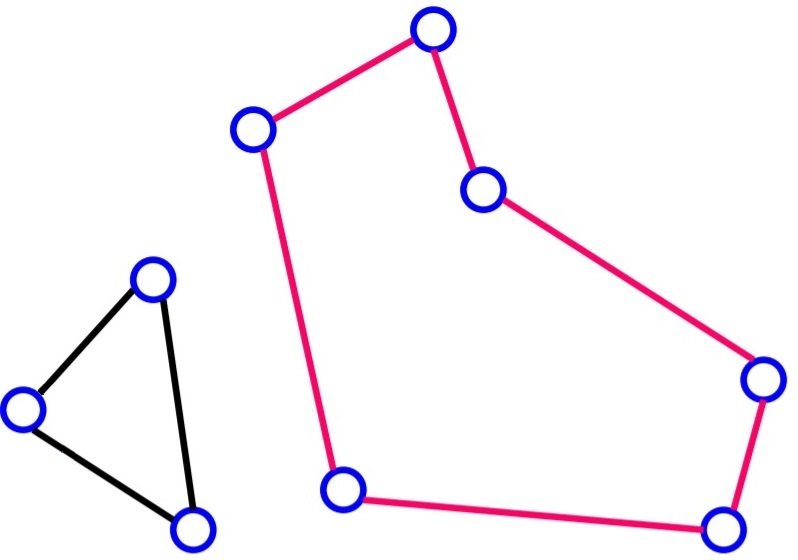
\includegraphics[scale=0.5]{subtour}  

Figura 1: Soluzione con due subtour
\end{center}

\vspace{2\baselineskip}

Una possibile formulazione per l'eliminazione dei subtour, detta appunto \textbf{subtour elimination}, risulta essere:

\begin{eqnarray}
&\displaystyle{\sum_{e \in E(S)}x_e \geq 1} \text{ , } \forall S \subsetneq V \text{ : } 1 \in S \text{ , } |S| \geq 2
\end{eqnarray}


Il vincolo (4) indica che se si considera un sottoinsieme $S \subsetneq V$, che includa il vertice numerato con il simbolo 1, allora il taglio di G indotto da S:

\begin{center}
$\delta(S) = $\{$ {[i,j]\in E : i \in S, j \notin S} $\} $ $
\end{center}

deve contenere almeno un lato appartenente ad $E$: poichè tutti i subtour violano tale vincolo la soluzione ottima non potrà contenerne al suo interno.  
Essendo il numero di questi vincoli pari ai sottoinsiemi $S$ distinti, il numero di tali vincoli risulta esponenziale rispetto alla dimensione dell'istanza. In particolare il valore di $S$, dato un numero $n$ di nodi, è $2^n$: questo perchè associando un bit ad ogni vertice (il cui valore definisce se appartiene o meno al sottoinsieme) un qualsiasi sottoinsieme risulta identificato da una sequenza di $n$ bit è quindi possibile definirne $2^n$ distinti. In realtà avendo noi imposto che il vertice 1 appartenga sempre ad ogni $S$ e che $S \subsetneq V$, si ha che il numero di vincoli di subtour risulti pari a  $2^{n-1} - 1$.

Una seconda formulazione equivalente per esprimere i vincoli di subtour è la seguente:

\begin{eqnarray}
&\displaystyle{\sum_{e \in E(S)}x_e \leq |S| - 1} \text{ , } \forall S \subsetneq V \text{ , } |S| \geq 2
\end{eqnarray}

La gestione di un numero esponenziale di vincoli implica in genere tempi di risoluzione troppo elevati. Nella pratica però non è necessario utilizzare tutti i vincoli di subtour elimination, è sufficiente considerarne un numero molto più ridotto. Non potendo conoscere in anticipo quali siano quelli essenziali sarà nostro compito progettare un opportuno separatore: ossia una funzione che fornita in ingresso una soluzione x* ottima per il modello corrente generi tutti i vincoli violati.


\vspace{2\baselineskip}
FILE DI INPUT
\vspace{2\baselineskip}


Le istanze del problema del Commesso Viaggiatore fornite in input al programma sono state selezionata da un libreria presente al seguente indirizzo web: 

\begin{center}
\href{http://elib.zib.de/pub/mp-testdata/tsp/tsplib/tsp/index.html}{http://elib.zib.de/pub/mp-testdata/tsp/tsplib/tsp/index.html}
\end{center}

Ogni istanza è memorizzata in un file di testo in un formato ben preciso, è stato quindi possibile progettare un opportuno parser che automaticamente riesca a estrapolare le informazioni contenute e popolare le strutture dati da noi create\footnote{Nessun altro tipo di input è supportato}. 

\vspace{2\baselineskip}



\vspace{2\baselineskip}
STRUTTURA DEL PROGETTO
\vspace{2\baselineskip}


I file che compongono il programma realizzato sono stati organizzati nel modo seguente; all' interno della cartella radice, da noi chiamata TSPCsharp, si sono create le seguenti sottocartelle:

\begin{itemize}
\item \textbf{Src} contenente il progetto di Visual Studio;
\item \textbf{Data} include le istanze del problema del commesso viaggiatore appartenenti alla TSPlib;
\item \textbf{Concorde} contenente i file sorgenti in linguaggio C del programma Concorde\footnote{Concorde è un software freeware sviluppato da \textbf{William Cook} per la risoluzione di problemi TSP} la cui trattazione è rimandata al Capitolo X.
\end{itemize}

Il software sviluppato è composto da dieci classi, riportiamo di seguito il nominativo di ognuna di esse:

\begin{itemize}
\item Instances
\item ItemList
\item PathGenetic
\item PathStandard
\item Point
\item Program
\item Tabu
\item TSP
\item TSPLazyConsCallback
\item Utility
\end{itemize}

Per le classi Point, Instances, Program, TSP e Utility verrà fornita una descrizione in questo capitolo, le rimanenti classi verranno presentate nei capitoli successivi poichè una loro trattazione risulterebbe in questo momento prematura. 


\vspace{2\baselineskip}
CLASSE POINT
\vspace{2\baselineskip}

La classe Point è stata realizzate al fine di memorizzare le coordinate in due dimensioni di un singolo nodo $n$, a tal fine sono presenti due variabili private, accessibili attraverso i propri metodi get e set, di tipo \textbf{double} chiamate rispettivamente \textbf{x} e \textbf{y}. Il costruttore della classe non fa altro che ricevere in input i valori da assegnare a queste ultime. La classe presenta inoltre un ulteriore metodo pubblico e statico chiamato \textbf{Distance} che permette il calcolo della distanza tra due nodi:

\begin{lstlisting}
    public static double Distance(Point p1, Point p2, string pointType)
\end{lstlisting}

\begin{itemize}
\item \textbf{p1}: Rappresenta il primo nodo;
\item \text{p2}: Rappresenta il secondo nodo;
\item \textbf{pointType}: Rappresenta il modo con cui il costo relativo al lato che congiunge p1 con p2 viene calcolato; i valori che questo parametro può assumere sono i seguenti:
    \begin{itemize}
    \item EUC\char`\_2D
    \item ATT
    \item MAN\char`\_2D
    \item GEO
    \item MAX\char`\_2D    
    \item CEIL\char`\_2D
    \end{itemize}
\end{itemize}

A titolo di esempio riportiamo il codice eseguito nel caso in cui pointType risulti uguale a EUC\char`\_2D dove il costo del lato deve risultare pari alla distanza euclidea dei due nodi. 

\begin{lstlisting}

 double xD = p1.X - p2.X;
 double yD = p1.Y - p2.Y;
 
 if (pointType == "EUC\_2D")
 {
     return (int)(Math.Sqrt(xD * xD + yD * yD) + 0.5);
 }
 else if ...
            
\end{lstlisting}

Per quanto riguarda gli altri metodi di calcolo della distanza rimandiamo il lettore alla visione del codice.

\vspace{2\baselineskip}
CLASSE INSTANCE
\vspace{2\baselineskip}

La classe Instance è stata creata per memorizzare tutti i dati caratterizzanti l'istanza del problema del Commesso Viaggiatore. La tabella sottostante fornisce un elenco di variabili ed array definite all'interno della classe assieme ad una loro breve descrizione. 


\begin{center}

    \begin{longtable}{ | p{4cm} | p{4cm} | p{7cm} |}
    \hline
    \begin{center} \textbf{Tipo di dato} \end{center} & \begin{center}  \textbf{Nome} \end{center}& 
    \begin{center} \textbf{Descrizione} \end{center}\\ \hline
    \begin{center} int \end{center} & \begin{center} nNodes \end{center}& \vfill Rappresenta il numero di nodi dell' istanza del problema del Commesso Viaggiatore.\vfill \\ \hline
    \begin{center} Point[ ] \end{center} & \begin{center} coord \end{center}& \vfill Vettore di Point contenente le coordinate di tutti i vertici del grafo.\vfill\\ \hline
    \begin{center} string \end{center} & \begin{center} edgeType \end{center}&\vfill Definisce la modalità con cui calcolare la distanza fra due nodi.\vfill \\ \hline
    \begin{center} double \end{center} & \begin{center} timeLimit \end{center}& \vfill Definisce la quantità massima di tempo che il programma dispone per il calcolo della soluzione.\vfill \\ \hline
    \begin{center} double \end{center} & \begin{center} inputFile \end{center}&\vfill Rappresenta il nome del file di input contenente l'istanza del problema del Commesso Viaggiatore. \vfill\\ \hline
    \begin{center} double \end{center} & \begin{center} tStart \end{center}& \vfill Rappresenta i secondi trascorsi dall'attivazione del cronometro al reale inizio delle operazioni di calcolo per la risoluzione del problema \vfill \\ \hline
    \begin{center} double \end{center} & \begin{center} xBest \end{center}& \vfill Rappresenta il costo della soluzione ottima restituira da cplex.\vfill \\ \hline
    \begin{center} double \end{center} & \begin{center} tBest \end{center}& \vfill Contiene la qantità di tempo impiegata per il calcolo della soluzione ottima. \vfill \\ \hline
    \begin{center} double \end{center} & \begin{center} bestSol \end{center}& \vfill Rappresenta la soluzione ottima ritornata da Cplex.\vfill \\ \hline
     \begin{center} double \end{center} & \begin{center} bestLb \end{center}& \vfill Rappresenta il miglior lower bound attualmente calcolato.\vfill \\ \hline
    \begin{center} double \end{center} & \begin{center} bestLb \end{center}& \vfill Rappresenta il miglior lower bound attualmente calcolato.\vfill \\ \hline
     \begin{center} double \end{center} & \begin{center} bestLb \end{center}& \vfill Rappresenta il miglior lower bound attualmente calcolato.\vfill \\ \hline
    \end{longtable}
\end{center}

\textit{xMin e yMin ... mi servivano per gnuplot ma dato che ho messo l'autoscale credo non servano più. per xBest ok}

L' unico metodo appartenente a questa classe, esclusi i vari getter e setter, è \textbf{Print}, la cui firma risulta essere:

\begin{lstlisting}
                  static public void Print(Instance inst)
\end{lstlisting}

dove:

\begin{itemize}
\item \textbf{inst}: oggetto della classe Instance contente tutti dati che descrivono l'istanza del problema del Commesso Viaggiatore fornita in ingresso dall' tente;
\end{itemize}

Tale metodo stampa a video le coordinate di tutti i nodi memorizzati dentro \textbf{inst}. Viene di seguito riportato il codice:

\begin{lstlisting}
for (int i = 0; i < inst.NNodes; i++)
    Console.WriteLine("Point #" + (i + 1) + "= (" + inst.Coord[i].X + "," + inst.Coord[i].Y + ")");
\end{lstlisting}

\vspace{2\baselineskip}

CLASSE PROGRAM

\vspace{2\baselineskip}

La classe Program contiene il metodo Main che, come noto, rappresenta il punto di inizio del programma: attraverso le funzionalità di Visual Studio esso riceve in input l'array \textbf{argv} di stringhe contenente i parametri di input forniti dall'utente come il nome del file contenente l'input ed il time limit per la sua risoluzione. Appartengono a questa classe anche i metodi \textbf{ParseInst} e \textbf{Populate}: rispettivamente forniscono il parser per \textbf{argv} ed il parser del file di ingresso indicato con conseguente inizializzazione delle coordinate dei nodi. Firma e implementazione di tali metodi è rimandata al successivo capitolo.\\
All'interno del metodo \textbf{Main} vengono eseguite in ordine le seguenti attività:
\begin{itemize}
    \item Creata una istanza della classe \textbf{Instance} ed invocati i due metodi precedentemente nominati.
    \item Creato un oggetto della classe \textbf{Stopwatch}. Questa classe è fornita direttamente da Visual Studio appartenente al Namespace \textbf{System.Diagnostics} è fornisce le funzionalità di un cronometro compatibile al multithreading.
    \item Invocato il metodo \textbf{TSPOpt} della classe \textbf{TSP} passandogli come parametri i due oggetti di tipo Instance e Stopwatch.
    \item In caso di risultato positivo (una soluzione del problema è stata trovata) viene mostrato a video il risultato ottenuto ed il tempo di calcolo trascorso.
    \item Viene effettuata una pulizia dei file creatisi durante l'esecuzione del problema.
\end{itemize}

In tutto il nostro progetto si è cercato di utilizzare il minor numero possibile di variabili globali, in particolare solo all'interno di questa classe ne sono state definite due di seguito descritte:

\begin{center}
    
    \begin{tabular}{ | p{1.5cm} | p{4cm} | p{2cm} | p{6.5cm} |}
        \hline
        \begin{center} \textbf{Tipo di dato} \end{center} & \begin{center}  \textbf{Nome} \end{center}& \begin{center} \textbf{Valore} \end{center} & \begin{center} \textbf{Descrizione} \end{center}\\ \hline
        \begin{center} int \end{center} & \begin{center} VERBOSE \end{center}& \begin{center} 5 \end{center} & Regola quanto output il programma mostra a video: si è scelto di condizionare l' esecuzione di molte righe di codice che producevano una stampa a video in base al valore assunto da questa variabile. Si è deciso di ristringere il suo valore da 1 a 9, quando assume il valore 9 viene riportato a video il maggior numero possibile di stampe. \\ \hline
        \begin{center} int \end{center} & \begin{center} TICKS\char`\_PER\char`\_SECOND \end{center} &  \begin{center}1000  \end{center}& Cplex utilizza i così detti ticks come unità di misura per il tempo di calcolo, questa costante indica quanti ne trascorrono in un secondo.\\ \hline
        
    \end{tabular}
\end{center}

\vspace{2\baselineskip}
CLASSE TSP
\vspace{2\baselineskip}

La classe \textbf{TSP} è stata pensata come il cuore del programma in quanto lo scheletro di tutti i metodi di risoluzione implementatisi trova al suo interno. Contiene un unico metodo pubblico che rappresenta quindi l'unico entry point per utilizzare questa classe: \textbf{TSPOpt}.

\begin{lstlisting}
static public bool TSPOpt(Instance instance, Stopwatch clock)
\end{lstlisting}

Come già specificato nella descrizione della classe Program, TSPOpt è invocato dal metodo Main e pertanto maggiori dettagli riguardanti i suoi parametri di ingresso possono essere trovati nella sezione precedente.\\
TSPOpt si preoccupa di istanziare i vari elementi utilizzati da tutti i metodi di risoluzione\footnote{Fatta eccezione per l'UserCutCallBack che è gestita esternamente da una DLL}, fornire all'utente un'interfaccia grafica che gli permetta di scegliere quale di questi ultimi voglia utilizzare e di conseguenza invoca il metodo privato della classe associato alla scelta effettuata.\\
Entrando nello specifico per quanto riguarda gli elementi inizializzati troviamo un oggetto della classe \textbf{Cplex} che come già accennato in precedenza ci permetterà di stabilire una connessione con il programma Cplex ed utilizzarlo per la risoluzione del modello matematico, ed un oggetto \textbf{Process} che sostanzialmente viene da noi utilizzato per inizializzare e comunicare con il programma \textbf{GNUPlot}\footnote{Per maggiori dettagli si veda la sezione dedicata a GNUPlot}.

\vspace{2\baselineskip}
CLASSE UTILITY
\vspace{2\baselineskip}

La classe Utility può essere considerata come una libreria: contiene al suo interno solamente metodi \textbf{statici} che si è deciso di raggruppare al suo interno per rendere il codice il più compatto e leggibile possibile.

\vspace{2\baselineskip}
INTERPRETAZIONE FILE DI INPUT
\vspace{2\baselineskip}

Lo sviluppo del programma è iniziato realizzando una opportuna funzione per interpretare correttamente i parametri di ingresso forniti dall'utente. Oltre al nome del file di testo contenente i dati relativi  all'istanza del problema che si vuole risolvere, all'utente è richiesto di fornite un time limit(espresso in secondi) e di scegliere con quale algoritmo risolvere l'istanza da esso fornita. Si è deciso di ricevere da riga di comando il nome del file e il time limit; per quanto riguarda la scelta dell'algoritmo risolutore ed eventuali parametri da esso richiesti si è preferito realizzare una semplice interfaccia grafica per favorire l'utente. 
Visual Studio, all'interno delle proprietà del progetto, permette di definire una stringa come parametro di ingresso per il programma. Questa viene automaticamente separata in sottostringhe utilizzando come separatore il carattere di spazio e fornito in ingresso al metodo Main. Allo stato attutale è gestita solamente la possibilità di fornire in ingresso il nome del file contenente i dati ed il timelimit per la ricerca della soluzione. Per ottenere una migliore organizzazione e chiarezza per il nostro lavoro è stato deciso di utilizzare questa regola per la costruzione della stringa di ingresso: ogni parametro inseritovi deve essere preceduto da una parola chiave che lo identifica il cui primo carattere deve essere '-'. Questa tecnica si rileverà utile anche in futuro nel caso si decidesse di ampliare la lista di parametri di ingresso.\\
La funzione che interpreta correttamente gli argomenti forniti in input dalla riga di comando è stata chiamata ParseInst ed ha la seguente intestazione:

\begin{lstlisting}
      static void ParseInst(Instance inst, string[] input) 
\end{lstlisting}


\begin{itemize}
\item \textbf{inst}: rappresenta il riferimento all'istanza della classe Instance dichiarata nel metodo Main, i valori letti vengono memorizzati al suo interno.
\item \textbf{input}: rappresenta un vettore contenente i parametri di input forniti da riga di comando dall'utente.
\end{itemize}


Il metodo è composto da un semplice ciclo for che scandisce il vettore \textbf{input} cercando una parola chiave, se trovata la stringa successiva viene memorizzata correttamente dentro \textbf{inst}: 

\begin{lstlisting}

for (int i = 0; i < input.Length; i++)
{
   if (input[i] == "-file")
   {
     //Expecting that the next value is the file name
       inst.InputFile = input[++i];
       continue;
    }
    if (input[i] == "-timelimit")
    {
      //Expecting that the next value is the time limit in seconds
       inst.TimeLimit = Convert.ToDouble(input[++i]);
       continue;
    }
}               
\end{lstlisting}

Nel caso in cui l' utente non fornisca il nome del file di input oppure il time limit viene lanciata una eccezione:

\begin{lstlisting}

if (inst.InputFile == null || inst.TimeLimit == 0)
     throw new Exception("File input name and/or timelimit are missing");

\end{lstlisting}


\vspace{2\baselineskip}
METODO POPULATE
\vspace{2\baselineskip}

Il metodo Populate è utilizzato per la lettura dei dati contenuti all'interno del file di input e soprattutto alla loro memorizzazione all'interno di un oggetto di tipo \textbf{Instance} in modo tale che una volta conclusosi il metodo questo contenga tutte le informazioni necessarie per la creazione del modello matematico.\\
I file di input presenta una struttura pressoché identica tra loro e cioè una divisione in sezioni identificate da parole chiave. Fatta eccezione per la sezione che descrive le coordinate dei nodi, tutte le altre si sviluppano in una sola riga la cui struttura è del tipo:

\begin{center}
<parolaChiave> : < valore> 
\end{center}

Di seguito sono riportati i valori che possono essere assunti dalle parole chiavi e il significato del contenuto della relativa sezione: 

\begin{itemize}
    \item NAME:<string> 
    \begin{itemize}
    \item nome con cui l' istanza è nota in letteratura.
    \end{itemize}
    \item TYPE:<string>
    
    \begin{itemize}     
    \item indica il tipo dell' istanza. Nel nostro ambito sarà sempre TSP.    
    \end{itemize}    
     
    \item \textbf{COMMENT:<string>} 
    \begin{itemize}    
    \item include informazioni aggiuntive, solitamente contiene il nome deli gli autori che hanno proposto l'                  istanza.
    \end{itemize}    
    
        
    \item \textbf{DIMENSION:<integer>} 
    \begin{itemize}
    \item indica il numero di nodi.
    \end{itemize}    
    
    \item \textbf{EDGE WEIGHT TYPE:<string>}
    \begin{itemize} 
    \item Definisce il modo con cui il costo del lato deve essere calcolato, i possibili valori  che può assumere                 il contenuto di questa sezione sono stati già presentati a pagina 7 durante la descrizione del metodo Distance.
    \end{itemize}    
    
    \item \textbf{NODE COORD SECTION}: 
    \begin{itemize}    
    
    \item Il contenuto di questa sezione si sviluppa in più righe; in ogni riga troviamo nell' ordine:
    \begin{itemize}
    \item Un numero progressivo intero positivo che comincia da 1 e che identifica il nodo. Osserviamo che anche se in input il primo nodo è numerato a partire da 1, nel vettore Point di inst le coordinate saranno memorizzate a partire dall'indice 0\footnote{Tale scelta è per mantenere una conformità con la metrica adottata dal linguaggio C\# per l'enumerazione degli elementi dei vettori, nel caso in cui le coordinate vengano visualizzate a video il loro indice viene comunque incrementato di uno}.
    \item Un numero reale positivo che definisce la coordinata x del nodo.
    \item Un numero reale positivo che identifica la coordinata y del nodo.
    \end{itemize}        
    \end{itemize}    
\end{itemize}

Il file di testo termina sempre con la stringa \textbf{EOF} che indica la fine del file di testo.

Per poter leggere il contenuto di un file è necessario inizializzare una nuova istanza della classe StreamReader passando come parametro al costruttore il percorso ove tale file è  collocato.


\begin{lstlisting}

StreamReader sr = new StreamReader("..\\..\\..\\..\\Data\\" + inst.InputFile)

\end{lstlisting}


Il metodo ReadLine() della classe StreamReader ritorna, come stringa, il contenuto di una intera riga del file la quale viene memorizzata all'interno di una variabile di tipo string chiamata \textbf{line}. Poichè si vuole leggere tutto il contenuto del file, è necessario invocare ReadLine() ciclicamente sull' oggetto \textbf{sr} finchè line risulta diversa da null oppure viene incontrata la parola chiave \textbf{EOF}.

\begin{lstlisting}

while ((line = sr.ReadLine()) != null)
{
    ...
    
    //This line signals the end of the file
    if (line.StartsWith("EOF"))
    {
    Instance.Print(inst);
    Console.WriteLine(line);
    //Correct end of the file
    break;
    }
    
    ...
}
\end{lstlisting}


Poichè ogni riga inizia con una nota parola chiave, per prelevare il contenuto di una sezione e memorizzarlo in un opportuno campo di inst, è sufficiente confrontare la prima stringa di ogni riga con una delle noti parole chiavi. Per far ciò si è  usato il metodo StartWith della classe String, la cui firma è:

\begin{lstlisting}

                    public bool StartWith(string value)

\end{lstlisting}

Questo metodo, applicato alla variabile line, determina se la prima stringa di line corrisponde alla stringa value specificata all'atto dell' invocazione del metodo. Nel caso in cui il confronto dia esito positivo, per prelevare il contenuto della sezione è necessario applicare i metodi IndexOf e Remove sempre alla variabile line; l'intestazione di tali metodi è riportata di seguito:


\begin{lstlisting}

               public int IndexOf(string value,int startIndex)

\end{lstlisting}

dove:

\begin{itemize}
    \item \textbf{value}: stringa da cercare.
    \item \textbf{startIndex}: posizione iniziale della ricerca.
\end{itemize}

\begin{lstlisting}

                public string Remove(int startIndex, int count)

\end{lstlisting}


dove:

\begin{itemize}
    \item \textbf{startIndex}: posizione da cui iniziare l'eliminazione dei caratteri.
    \item \textbf{count}: numero di caratteri da eliminare.
\end{itemize}

Per quanto detto, risulta immediata la comprensione del codice necessario per prelevare il contenuto della sezione e memorizzarlo dentro un oggetto di tipo \textbf{Instance} chiamando il metodo setter adeguato:

\begin{lstlisting}

                inst.SetterName = (line.Remove(0, line.IndexOf(:) + 2));

\end{lstlisting}

Il codice riportato deve chiaramente effettuare un cast per i tipi diversi da string, i metodi necessari sono già disponibili all'interno della classe \textbf{Convert} di C\#.

Una volta che ci troviamo all'interno della sezione \textbf{NODE COORD SECTION} la lettura delle coordinate viene eseguita eseguendo ciclicamente il seguente codice:

\begin{lstlisting}

string[] elements = line.Split(new[]{ ' ' } , StringSplitOptions.RemoveEmptyEntries);

int i = Convert.ToInt32(elements[0]);

inst.Coord[i - 1] = new Point(Convert.ToDouble(elements[1].Replace(".", ",")), Convert.ToDouble(elements[2].Replace(".",",")));
\end{lstlisting}

Il metodo Split della classe String ritorna un array contenente in ogni elemento una sottostringa della stringa a cui tale metodo è applicato. Le sottostringhe vengono estratte dalla stringa in base ai caratteri delimitatori specificati all'atto dell'invocazione del metodo, quest'ultimo ha diversi overload: quello di nostro interesse è riportato di seguito.

\begin{lstlisting}

     public string[] Split(char[] separator, StringSplitOptions options)

\end{lstlisting}

dove:

\begin{itemize}
\item \textbf{separator}: array i cui elementi definiscono i separatori della stringa. Nel nostro caso è un array con un solo elemento contenente il carattere \textipa{"}   \textipa{"}.
\item \textbf{options}: A questo parametro possono essere passate solo i seguenti due valori dell' enumerazione StringSplitOptions:

\begin{itemize}

\item \textbf{StringSplitOptions.RemoveEmptyEntries}: indica che gli elementi dell'array ritornato non possono essere stringhe vuote. Questo è l'opzione da noi selezionata.
\item \textbf{StringSplitOptions.None}: indica che gli elementi dell'array ritornato possono essere stringhe vuote.

\end{itemize}

\end{itemize}

Ogni coordinata letta viene tradotta in un oggetto di tipo \textbf{Point} il quale è a sua volta memorizzato all'interno del vettore \textbf{Coord} dell'oggetto di tipo \textbf{Instance} nella posizione indice letta.

Come nota conclusiva specifichiamo che C\# utilizza come separatore tra parte intere e parte decimale di un numero il carattere \textipa{"},\textipa{"} e non il carattere \textipa{"}.\textipa{"} utilizzato per nei file di input. E' quindi necessaria una modifica delle stringhe lette attraverso il metodo non statico della classe string:

\begin{lstlisting}

     public string Replace(string oldValue, string newValue)
)

\end{lstlisting}
dove:
\begin{itemize}
    \item \textbf{oldValue}: stringa sa sostituire;
    \item \textbf{newValue}: stringa con cui sostituire tutte le occorrenze di oldValue.
\end{itemize}

\vspace{2\baselineskip}
COSTRUZIONE DEL MODELLO
\vspace{2\baselineskip}

In questo paragrafo vedremo come è possibile creare da programma un modello matematico attraverso l'uso di alcune routine appartenenti alla libreria di Cplex. Esula dallo scopo di questa tesi fornire al lettore una descrizione del funzionamento di Cplex da iterativo.


\vspace{2\baselineskip}
COSTRUZIONE MODELLO IN C
\vspace{2\baselineskip}

Per istanziare un nuovo modello di programmazione lineare è necessario inizializzare un \textbf{environment} di Cplex utilizzando la funzione \textbf{CPXopenCPLEX} la quale ritorna un puntatore all'environment creato, la firma di tale funzione è:


\begin{lstlisting}

                CPXENVptr CPXopenCPLEX(int* status\_p)

\end{lstlisting}

dove:

\begin{itemize}
\item \textbf{status\char`\_p}: puntatore ad una variabile di tipo intero usato per ritornare un eventuale codice di errore.
\end{itemize}


Ad un enviroment è possibile associare uno o più modelli attraverso il comando \textbf{CPXcreateprob}, la cui intestazione è:

\begin{lstlisting}

    CPXLPptr CPXcreateprob(CPXCENVptr env, int * status\_p, const char * probname\_str

\end{lstlisting}


dove:

\begin{itemize}
    \item \textbf{env}: puntatore all'environment sul quale si è deciso di creare il modello;
    \item \textbf{status\char`\_p}: puntatore ad una variabile di tipo intero usato per ritornare un eventuale codice di errore;
    \item \textbf{probname\char`\_str}: rappresenta un array di caratteri che definisce il nome del modello creato.
\end{itemize}

Tale funzione ritorna un puntatore al modello creato: questo risulta vuoto poichè privo di funzione obbiettivo, variabili e vincoli.\\

Procediamo quindi al loro inserimento partendo definendo contemporaneamente le variabili e il loro coefficiente nella funzione obiettivo; è possibile procedere in più modi, quello da noi scelto è di utilizzare la funzione \textbf{CPXnewcols} la cui firma è:


\begin{lstlisting}

int CPXnewcols (CPXENVptr env,CPXLPptr lp,int ccnt,double *obj, double *lb, double *ub, char *ctype, char **colname);

\end{lstlisting}

dove:

\begin{itemize}
\item \textbf{env} : puntatore all'enviroment di Cplex nel quale vuole essere inserito il modello.
\item \textbf{lp} : puntatore al problema di programmazione lineare.
\item \textbf{ccnt} : intero che indica il numero delle nuove variabili che vengono aggiunte al problema.
\item \textbf{obj} : array contenente per ogni variabile il relativo coefficiente 
\item \textbf{lb} : array di lunghezza ccnt contenente il lower bound di ogni variabile aggiunta.
\item \textbf{ub} : array contenente l'upper bound di ogni variabile aggiunta.
\item \textbf{ctype} : array di lunghezza ccnt contenente il tipo di ogni variabile. I valori che un elemento di questo array può assumere sono:
\begin{itemize}
    \item \textbf{\textipa{"}C\textipa{"}}: variabile continua
    \item \textbf{\textipa{"}B\textipa{"}}: variabile binaria
    \item \textbf{\textipa{"}I\textipa{"}}: variabile intera
\end{itemize}
\item \textbf{colname} : array di lunghezza ccnt contenente puntatori ad array di char, a sua volta ognuno di essi deve contenere il nome della variabile aggiunta al modello.
\end{itemize}

Per motivi di semplicità non andremo ad inserire tutte le variabili contemporaneamente ma una ad una.\\

E' giunto quindi il momento di parlare di quali variabili vogliamo aggiungere al nostro modello tenendo presente che il medesimo discorso sarà applicato anche per la parte in C\#. Sappiamo che per ogni coppia di nodi (i,j)\footnote{Ricordiamo che i deve essere diverso da j in quanto per i problemi da noi considerati i cappi non sono ammessi} esiste un unico lato che li collega e che quest'ultimo è privo di direzione. Si presenta quindi la necessità di definire una convenzione per l'assegnazione del nome ai vari lati. La scelta adottata è la seguente: considerando due generici nodi \textbf{i} e \textbf{j} allora il loro lato sarà chiamato \textbf{x(i,j)} se $i<j$ oppure \textbf{x(j,i)} se $j<i$\footnote{Notiamo che per quanto espresso nella nota precedente non ha senso considerare il caso $i=j$}.\\
Questa convenzione offre anche un importante spunto per decidere con quale ordine memorizzare i vari parametri delle variabili (nome, coefficiente, lower bound ecc..): date due coppie distinti di nodi (i,j) e (v,w)\footnote{dove assumiamo $i<j \& v<W$} la posizione di memoria in cui viene memorizzata l'informazione riguardante la prima coppia è \textbf{inferiore} rispetto alla seconda se e solo se $(i<v) || (i==v \& j<w)$. In altre parole saranno memorizzate in ordine le informazioni per i nodi (1,2), (1,3), ..., (2,3), (2,4), ..., (n-1,n).\\
Una ulteriore considerazione necessaria è la seguente: come mostrato poco fa il metodo \textbf{CPXnewcols} si aspetta il passaggio di diversi array mentre noi vorremmo utilizzare semplici variabili. La soluzione è molto semplice e consiste nell'anteporre il carattere \& prima di ogni variabile in questo modo stiamo in realtà passando un puntatore alla sua locazione di memoria.\\

Le operazioni descritte sono state realizzate tramite il seguente codice:

\begin{lstlisting}

double zero = 0.0; // one = 1.0;     
char binary = 'B';

char **cname = (char **)calloc(1, sizeof(char *));        // (char **) required by cplex...
cname[0] = (char *)calloc(100, sizeof(char));

// add binary var.s y(i,j)      

for (int i = 0; i < inst->nNodes; i++)
{
    for (int j = i + 1; j < inst->nNodes; j++)//Mi interessano solo le coppie con i<j
    {
        sprintf(cname[0], "x(%d,%d)", i + 1, j + 1);
        double obj = dist(inst->coord[i], inst->coord[j], inst->edgeType);
        double ub = 1.0;
        if (CPXnewcols(env, lp, 1, &obj, &zero, &ub, &binary, cname)) printError(" ... errato CPXnewcols su x");//Aggiugo una variabile al modello
        if (CPXgetnumcols(env, lp) - 1 != xPos(i, j, inst)) printError(" ... errata posizione per x");//Serve solo per controllare se la funzione xPos è corretta
    }
}

\end{lstlisting}

La funzione chiamata xPos  riceve in ingresso un lato (i,j) del grafo e restituisce l'indice della variabile Cplex associata a quest'ultimo. Dato che risulta possibile effettuare errori nella realizzazione di questa funzione, in questo punto del codice è  utile effettuare un controllo se il valore ritornato da xPos coincide con quello aspettato,in caso contrario viene sollevata una eccezione. Firma e dettagli implementativi di xPos saranno forniti nel paragrafo successivo in quanto è definita anche in C\#.\\

Una volta definite le variabili è necessario creare i vincoli: per far ciò si è utilizzata la funzione \textbf{CPXnewrows}, la cui firma è:

\begin{lstlisting}
int CPXnewrows(CPXCENVptr env, CPXLPptr lp, int rcnt, const double * rhs, const char * sense, const double * rngval, char ** rowname)
\end{lstlisting}

dove:

\begin{itemize}
\item \textbf{env}: puntatore all'enviroment di Cplex nel quale vuole essere inserito il modello.
\item \textbf{lp}: puntatore al problema di programmazione lineare.
\item \textbf{rcnt}: intero che definisce il numero di nuovi vincoli aggiunti al modello.
\item \textbf{rhs}: array di lunghezza rcnt contenente il termine noto di ogni vincolo.
\item \textbf{sense}: array di lunghezza rcnt i cui elementi possono assumere i seguenti valori:

\begin{itemize}
\item \textbf{\textipa{"}L\textipa{"}}: indica che il vincolo è una disuguaglianza il cui segno è  $\leq$
\item \textbf{\textipa{"}E\textipa{"}}: indica che il vincolo è una uguaglianza
\item \textbf{\textipa{"}G\textipa{"}}: indica che il vincolo è una disuguaglianza il cui segno è $\geq$
\item \textbf{\textipa{"}R\textipa{"}} : indica che il vincolo è limitato 
\end{itemize}

\item \textbf{rngval}: variabile di tipo double contenente il valore 1.0;
\item \textbf{rowname}: variabile di tipo char che assume il valore costante \textipa{"}B\textipa{"};
\end{itemize}

Anche in questo caso anzichè aggiungere tutti i vincoli in una singola iterazione, risulta più semplice aggiungere un vincolo per volta invocando il metodo tante volte quante sono i vincoli da aggiungere.

\vspace{2\baselineskip}
COSTRUZIONE E RISOLUZIONE DEL MODELLO MATEMATICO IN C\#
\vspace{2\baselineskip}

Per poter creare un modello matematico in Cplex, utilizzando come linguaggio di programmazione C\# è necessario creare inizialmente una istanza della classe \textbf{Cplex}:

\begin{lstlisting}
                           Cplex cplex = new Cplex();
\end{lstlisting}

Per creare il modello si associano, tramite opportune funzioni che descriveremo in questo paragrafo, all'istanza creata la funzione obbiettivo,le variabili e i vincoli del modello. 

In C\# le variabili del modello sono oggetti il cui tipo deve implementare l'interfaccia \textbf{INumVar}. Non è necessario creare da noi una nuova classe infatti ci viene fornito il metodo \textbf{NumVar} della classe \textbf{Cplex}:

\begin{lstlisting}
public virtual INumVar NumVar(double lb, double ub, NumVarType type, string name)
\end{lstlisting}

dove:

\begin{itemize}
\item \textbf{lb}: Rappresenta il lower bound della variabile creata;
\item \textbf{ub}: Rappresenta l' upper bound della variabile creata;
\item \textbf{type}: Questo campo determina il tipo della variabile, può assumere i seguenti valori:
\begin{itemize}
\item \textbf{NumVarType.Int}: Nel caso di variabile intera;
\item \textbf{NumVarType.Int}: Nel caso di variabile binaria;
\item \textbf{NumVarType.Float}: Nel caso di variabile continua;
\end{itemize}
\item \textbf{name}: Nome identificativo della variabile.
\end{itemize}

Che come si può notare nella firma ha come tipo di ritorno un tipo di oggetto che implementa l'interfaccia da noi desiderata. Vedremo nel seguito della trattazione quanto utili risultano essere le funzionalità offerta de quest'ultima.\\
Introduciamo ora una seconda interfaccia \textbf{ILinearNumExpr} che come si può intuire viene implementata da oggetti che vogliono definire una espressione lineare. Anche in questo caso ci viene incontro la classe \textbf{Cplex} attraverso il metodo \textbf{LinearNumExpr}:
\begin{lstlisting}
                ILinearNumExpr expr = cplex.LinearNumExpr();
\end{lstlisting}

La variabile \textbf{expr} rappresenta quindi una espressione lineare che deve essere definita come:

$$\displaystyle{\sum_{i = 1}^n a_i x_i} $$

dove \textbf{$x\_i$} sono variabili di tipo \textbf{INumVar} mentre \textbf{$a\_i$} è un coefficiente di tipo \textbf{double}. Per aggiungere all'oggetto \textbf{expr} una variabile del modello è necessario utilizzare il metodo \textbf{AddTerm} la cui intestazione è:

\begin{lstlisting}
                   void AddTerm(INumVar var,double coef)
\end{lstlisting}

dove:

\begin{itemize}
\item \textbf{var}: variabile da aggiungere all'espressione;
\item  \textbf{coeff}: coefficiente della variabile aggiunta all'espressione.
\end{itemize}

L'implementazione da noi fornita per quanto riguarda la funzione obiettivo è la seguente:

\begin{lstlisting}
//Populating objective function

for (int i = 0; i < instance.NNodes; i++)
{
  //Only links (i,j) with i < j are correct
  
  for (int j = i + 1; j < instance.NNodes; j++)
  {
      //zPos returns the correct position where to store the variable corresponding to the actual link (i,j)
           
     int position = zPos(i, j, instance.NNodes);
           
     z[position] = cplex.NumVar(0, 1, NumVarType.Int, "x(" + (i + 1) + "," + (j + 1) + ")");
         
     expr.AddTerm(z[position], Point.Distance(instance.Coord[i], instance.Coord[j], instance.EdgeType));      
   }
}

\end{lstlisting}

Espressioni lineari definite in questo modo possono essere utilizzate sia per definire la funzione obiettivo del modello ma anche per i suoi vincoli.\\
Nel primo caso risulta sufficiente invocare i metodi non statici \textbf{AddMinimize} oppure \textbf{AddMaximize} della classe \textbf{Cplex} che rispettivamente definiscono una funzione obiettivo da minimizzare o da massimizzare, nel nostro caso:            


\begin{lstlisting}
                         cplex.AddMinimize(expr);         
\end{lstlisting}

Per quanto riguarda i vincoli è necessario utilizzare i metodi \textbf{AddEq}, \textbf{AddLe}, \textbf{AddGe} che rispettivamente aggiungono al modello una equazione, una disequazione avente segno $\leq$, una disequazione avente segno $\geq$.\\
Nel nostro caso poichè ogni vincolo è una equazione riportiamo di seguito la firma della relativa funzione:

\begin{lstlisting}
public virtual IRange AddEq(INumExpr e,double v,string name)
\end{lstlisting}

dove:

\begin{itemize}
    \item \textbf{e}: Espressione contenente le variabili del vincolo;
    \item \textbf{v}: Termine noto del vincolo;
    \item \textbf{name}: Nome identificativo del vincolo.
\end{itemize}

Il codice completo diventa quindi:

\begin{lstlisting}

for (int i = 0; i < instance.NNodes; i++)
{
 //Resetting expr
  expr = cplex.LinearNumExpr();

  for (int j = 0; j < instance.NNodes; j++)
  {
   //For each row i only the link (i,j) or (j,i) has coefficent 1
   //xPos return the correct position where link is stored inside the vector x
    
    if (i != j)//No loops with only one node
       expr.AddTerm(x[xPos(i, j, instance.NNodes)], 1);               
  }

//Adding to the model the current equation with known term 2 and name degree(<current i node>)
cplex.AddEq(expr, 2, "degree(" + (i + 1) + ")");
}

\end{lstlisting}

Spiegato come è possibile creare un modello C\# risulta comprensibile la scelta di realizzare un'opportuna funzione, chiamata \textbf{BuilModel} appartenente alla classe \textbf{Utility}, che produce il modello matematico del Commesso Viaggiatore risolubile da Cplex:

\begin{lstlisting}
public static INumVar[] BuildModel(Cplex cplex, Instance instance, int nEdges)
\end{lstlisting}

dove:

\begin{itemize}
\item \textbf{cplex}: oggetto sul quale si definirà il modello matematico(funzione obbiettivo,variabili e vincoli)
\item \textbf{instance}: oggetto contenente tutti i dati inerenti all'istanza del Commesso Viaggiatore fornita in ingresso dall' utente.
\item \textbf{nEdges}: Parametro la cui spiegazione è rimandata al capitolo...
\end{itemize}

Passiamo infine a descrivere i metodi necessari per risolvere il modello, ottenere il costo e la soluzione ottima calcolata da Cplex.\\

Per risolvere il modello è sufficiente invocare, sull'oggetto di classe Cplex dove è stato definito, il metodo \textbf{Solve}:

\begin{lstlisting}
                         cplex.Solve();
\end{lstlisting}

Una volta avviata la risoluzione, Cplex fornisce in automatico informazioni sul processo stampate nello standard output da noi definito\footnote{Se non viene modificato di default risulta essere la classica console del progetto C\#}: inizialmente troviamo le impostazioni di risoluzione selezionate come ad esempio il numero di Thread .., successivamente ..  .\\
Terminata l'operazione il costo della soluzione è memorizzato all'interno della variabile \textbf{ObjValue} di tipo \textbf{double} del solito oggetto \textbf{cplex}:

\begin{lstlisting}
                        cplex.ObjValue; 
\end{lstlisting}

Naturalmente è anche possibile conoscere il valore assunto da ogni variabile nella soluzione fornitaci da Cplex tramite il metodo \textbf{GetValues} della classe \textbf{Cplex}:

\begin{lstlisting}
                public virtual double GetValues(INumVar[] var)
\end{lstlisting}

dove:

\begin{itemize}
\item \textbf: rappresenta il vettore contenente tutte le variabile appartenenti al modello.
\end{itemize}

\'E presente anche l'analogo metodo per accedere al valore di una sola variabile \textbf{GetValue}. Il suo utilizzo è da noi altamente sconsigliato in quanto sperimentalmente è stato da verificato che ciclare quest'ultimo metodo impiega un tempo molto maggiore rispetto al semplice \textbf{getValues}.



------------------------------------------------------------------
Qui bisogna aprire un capitolo nuovo con una breve introduzione, dire che si passa ora ad esporre i metodi utilizzati per gestire i vincoli di subtour elimination
------------------------------------------------------------------


\vspace{2\baselineskip}
METODO LOOP
\vspace{2\baselineskip}

Il primo metodo sperimentato prende il nome di \textbf{LOOP}.
-------------------------------------------------------------
Va messa un pò di storia!!!!!!
-------------------------------------------------------------
L'idea alla sua base è molto semplice ed è la seguente: inizialmente il modello fornito non deve contiene alcun vincolo di subtour elimination ed una volta risolto si procedere ad analizzare la soluzione ottima trovata. Se questa presenta dei subtour il modello viene ampliato inserendovi gli appositi vincoli per eliminarli e si procede ad una sua nuova risoluzione. Viene da se che quest'ultimo passo va ripetuto fino a quando la soluzione proposta non risulta accettabile e quindi priva di subtour\footnote{Da qui deriva il nome del metodo in quanto la soluzione consiste in un loop delle stesse operazioni}.\\\'E importante far notare che ogni iterazione del loop i vincoli aggiunti nella precedente sono ovviamente mantenuti.\\
In questo modo siamo sicuri di aver aggiunto al nostro modello solo i vincoli strettamente necessari il che non assicura che essi non siano un numero esponenziale.\\

Per poter implementare il metodo Loop risulta quindi evidente la necessità di sviluppare un'opportuna funzione in grado di individuare la presenza di subtour all'interno di una generica soluzione proposta e di generarne gli opportuni vincoli per eliminarli.\\
In letteratura esistono molteplici modi per eseguire tali operazioni, quella da noi adottata si rifà all'algoritmo di \text{Kruskal} per trovare un albero a costo minimo in un grafo connesso con lati non orientati\footnote{Nello specifico la parte di nostro interesse è quella che impedisce la formazione di più componenti connesse}.\\
La tecnica da noi adottata è stata quella di creare due metodi chiamati \textbf{InitCC} e \textbf{UpdateCC}: il primo serve solamente come inizializzazione per le strutture dati utilizzate dal secondo il quale, se invocato una volta per ogni lato appartenente alla soluzione attuale ne trova tutte le componenti connesse indicando anche quali lati sono a loro appartenenti. I dettagli riguardo le loro implementazioni sono visibili nella appendice di questo testo, per ora specifichiamo solamente che al termine dell'utilizzo del metodo \textbf{UpdateCC} i seguenti oggetti:

\begin{lstlisting}

        List<ILinearNumExpr> rcExpr = new List<ILinearNumExpr>();
        List<int> bufferCoeffRC bufferCoeffRC = new List<int>();

\end{lstlisting}

risultano essere costruiti, in particolare \textbf{rcExpr} contiene le espressioni dei subtour elimination mentre invece \textbf{bufferCoeffRC} contiene il numero di lati appartenenti ad ogni subtour e quindi il termine noto delle precedenti espressioni\footnote{Il codice assume che l'espressione di indice $i$ presente all'interno di \textbf{rcExpr} abbia il proprio termine noto nella posizione di indice $i$ dentro \textbf{bufferCoeffRC}}.\\
Se all'interno di \textbf{rcExpr} è presente una espressione sola significa che la soluzione attuale è valida e quindi ottima per il problema, al contrario si deve procedere all'inserimento dei vincoli con un semplice ciclo for:

\begin{lstlisting}
                
for (int i = 0; i < rcExpr.Count; i++)
  cplex.AddLe(rcExpr[i], bufferCoeffRC[i] - 1);
              
\end{lstlisting}

\vspace{2\baselineskip}
METODI UpdateCC e InitCC
\vspace{2\baselineskip}

Come già specificato nella sezione riguardo il metodo \textbf{LOOP} questi due metodi di supporto appartenenti alla classe \textbf{Utility} hanno il compito di individuare tutte le componenti connesse (che da ora in avanti abbrevieremo con \textbf{cc}) di una generica soluzione proposta.\\
Prima di passare alla implementazione vera e propria introduciamoli ad alto livello: inizialmente si vuole assumere l'esistenza di $n$ \textbf{cc} distinte, ognuna di esse contenente un nodo della soluzione. Questo è il compito della dalla funzione \textbf{InitCC}.\\
Successivamente per ogni lato della soluzione si vuole analizzare a quali \textbf{cc} sono assegnati i due nodi che lo caratterizzano. Se queste sono differenti vanno unificate in modo tale che tutti i nodi appartenenti, ad esempio
, alla seconda ora appartengano tutti alla prima. Nel caso in cui invece le due \textbf{cc} coincidano significa che abbiamo trovato un subtour e il relativo vincolo di eliminazione deve essere definito. Tutte questo è invece compito del metodo \textbf{UpdateCC}.

Iniziamo quindi l'analisi del codice necessario. Per prima cosa si necessita di un vettore di interi che contenga all'indice $i-esimo$ l'identificativo della \textbf{cc} alla quale appartiene il nodo $i$\footnote{Per semplicità si è deciso di identificare ogni \textbf{cc} con un valore intero univoco}. L'inizializzazione di questo vettore viene fornita da \textbf{InitCC}:

\begin{lstlisting}

public static void InitCC(int[] cc)
{
    for (int i = 0; i < cc.Length; i++)
    {
        cc[i] = i;
    }
}

\end{lstlisting}

Passiamo ora al metodo \textbf{UpdateCC} che presenta la seguente firma:

\begin{lstlisting}

public static void UpdateCC(Cplex cplex, INumVar[] z, List<ILinearNumExpr> rcExpr, List<int> bufferCoeffRC, int[] relatedComponents, int i, int j)

\end{lstlisting}

dove:

\begin{itemize}
    \item \textbf{cplex}: oggetto contenente il modello matematico corrente, eventualmente necessario per la creazione del vincolo di subtour elimination;
    \item \textbf{z}: vettore contenente le variabili del modello, eventualmente necessario per la creazione del vincolo di subtour elimination;
    \item \textbf{rcExpr}: Lista all' interno della quale vengono memorizzate le espressioni contenenti le variabili del vincolo di subtour;
    \item \textbf{bufferCoeffRC}: Lista contenente i termini noti dei vincoli di subtour;
    \item \textbf{relatedComponents}: vettore che definisce per ogni nodo del grafo la relativa componente connessa;
    \item \textbf{i}: Nodo che con il parametro j forma il lato (i,j);
    \item \textbf{j}: Nodo che con il parametro i forma il lato (i,j).
\end{itemize}

La funzione UpdateCC viene invocata dal metodo Loop $n$ volte, alla k-esima invocazione riceve in ingresso il k-esimo lato appartenente alla soluzione ottima del modello corrente. Per verificare se il lato ricevuto genera un subtour nel grafo G=(V,T*), dove T* contiene i precedenti $k-1$ lati controllati, si verifica se i vertici del lato appartengono alla medesima componente connessa. Nel caso in cui i due vertici non appartengono alla medesima componente connessa, è necessario aggiornare le componenti connesse dei vertici per l' invocazione successiva del metodo, viceversa si è  individuato un subtour caratterizzato dai nodi aventi come componente connessa la medesima dei nodi i e j.

A livello implementativo si è utilizzato un array di interi chiamato relatedComponents, di dimensione pari al numero di vertici del grafo, come struttura dati necessaria per fotografare le componenti connesse del grafo G=(V,T*); relatedComponents contiene all' indice j la componente connessa del nodo j. La funzione InitCC, invocata ad ogni iterazione del metodo Loop, ha il compito di inizializzare relatedComponents associando ad ogni nodo una componente connessa diversa: in particolare si è  scelto di associare al nodo j la componente connessa j. Passiamo ora ad analizzare come è  stato nella pratica implementato il metodo UpdateCC, la sua intestazione è la seguente:

\begin{lstlisting}

public static void UpdateCC(Cplex cplex, INumVar[] z, List<ILinearNumExpr> rcExpr, List<int> bufferCoeffRC,int[] relatedComponents, int i, int j)

\end{lstlisting}

dove:
\begin{itemize}
\item cplex: oggetto contenente il modello matematico corrente;
\item z: vettore contenente le variabili del modello;
\item rcExpr: Lista all' interno della quale vengono memorizzate le espressioni contenenti le variabili del vincolo di subtour;
\item bufferCoeffRC: Lista contenente i termini noti dei vincoli di subtour;
\item relatedComponents: vettore che definisce per ongi nodo del grafo la relativa componente connessa;
\item i: Nodo che con il parametro j forma il lato [i,j];
\item j: Nodo che con il parametro i forma il lato [i,j].
\end{itemize}

Il caso in cui non si crei un subtour è gestito molto semplicemente in questo modo:

\begin{lstlisting}

if (relatedComponents[i] != relatedComponents[j])
{
    for (int k = 0; k < relatedComponents.Length; k++)
    {
        if ((k != j) && (relatedComponents[k] == relatedComponents[j]))
        {
            //Same as Kruskal
            relatedComponents[k] = relatedComponents[i];
        }
    }
    //Finally also the vallue relative to the Point i are updated
    relatedComponents[j] = relatedComponents[i];
}

\end{lstlisting}

Dove per convenzione si è deciso di inglobare la \textbf{cc} del nodo $j$ in quella del nodo $i$.\\
Il secondo caso è invece gestito nel seguente modo:

\begin{lstlisting}

else
{
    ILinearNumExpr expr = cplex.LinearNumExpr();

    //cnt stores the # of nodes of the current related components
    int cnt = 0;

    for (int h = 0; h < relatedComponents.Length; h++)
    {
        //Only nodes of the current related components are considered
        if (relatedComponents[h] == relatedComponents[i])
        {
            //Each link involving the node with index h is analized
            for (int k = h + 1; k < relatedComponents.Length; k++)
            {
                //Testing if the link is valid
                if (relatedComponents[k] == relatedComponents[i])
                {
                    //Adding the link to the expression with coefficient 1
                    expr.AddTerm(z[zPos(h, k, relatedComponents.Length)], 1);
                }
            }
            cnt++;
        }
    }
    //Adding the objects to the buffers
    rcExpr.Add(expr);
    bufferCoeffRC.Add(cnt);
}

\end{lstlisting}

Ripetere il metodo \textbf{UpdateCC} una ed una sola volta per ogni lato appartenente alla soluzione corrente ci assicura che le due liste \textbf{rcExpr} e \textbf{bufferCoeffRC} contengano tutti i dati per implementare i subtour elimination desiderati.


\vspace{2\baselineskip} 
METODO LOOP CON PRIMA FASE EURISTICA 
\vspace{2\baselineskip} 

Il metodo Loop, essendo un algoritmo esatto, produce sistematicamente una soluzione che risulta essere un ottimo globale per l' istanza del Problema del Commesso Viaggiatore che si presta a risolvere. L' inconveniente principale, che tipicamente accomuna questa categoria di algoritmi, riguarda l' elevato tempo che essi impiegano nel calcolare un ottimo globale per istanze con un numero di nodi elevato. In particolare, per quanto riguarda il problema del Commesso Viaggiatore, ciò è dovuto nella crescita esponenziale del numero di vincoli di subtour all' aumentare del numero di nodi del grafo. Nonostante il metodo Loop aggiunga al modello solamente i vincoli strettamente necessari, il numero di iterazione che deve compiere per determinarli tutti, per istanze di grandi dimensioni, risulta notevole. Per tale ragione si è pensato di progettare una \textbf{fase euristica} dell' algoritmo che anticipi la \textbf{fase esatta}. La fase euristica è caratterizzata dalla riduzione del numero di vincoli di interezza; in particolare per ogni nodo, si \textbf{fissano} a 0 tutte le variabili corrispondenti a lati che incidono su di esso tranne per le \textbf{m} variabili relative agli \textbf{m} lati più corti. Dato un MIP, qualora si rilassa uno o più vincoli del modello, il problema che si ottiene prende il nome di subMIP.

Fissando la stragrande maggioranza delle variabili, che passano da O(n^2) ad al più 10m, il numero di nodi dell' albero decisionale diminuisce (poichè diminuiranno le operazioni di branching) velocizzando così l' algoritmo Branch and cut eseguito da Cplex. In questa fase del metodo Loop, il modello si arricchisce di tagli i quali saranno molto buoni poichè le variabili che partecipano al taglio sono le principali candidate a far parte della soluzione ottimale. 

Una volta che Cplex termine di calcolare la soluzione del subMIP, che indicheremo con \textbf{x*}, l' upper bound di tutte le variabili viene ripristinato al valore 1: il modello così ottenuto risulta essere quello originale contenente però tutti i vincoli di subtour ereditati dalla fase euristica. Ha così inizio la fase esatta dell' algoritmo in cui a Cplex si fornisce tale modello: qualora \textbf{x*} coincida con l' ottimo globale è sufficiente una sola iterazione del metodo Loop, altrimenti saranno necessarie \textbf{t} iterazioni. Il valore di \textit{t} determina la bontà o meno dell' metodo: se \textit{t} risulta, relativamente all' istanza,  grande significa che il tempo impiegato nella fase euristica dell' algoritmo non è risultato particolarmente produttivo. 

Al fine di confrontare le prestazioni e verificare se effettivamente con una prima fase euristica mediamente migliorano, quest' ultima risulta attivabile o meno dall' utente tramite l' interfaccia grafica realizzata.

Il parametro \textit{m} non può essere definito a priori poichè è un parametro euristico il cui valore "ottimale" dipende dall' istanza che si vuole risolvere: in particolare dipende da come sono posizionati i nodi e dal numero di quest' ultimi. Per i motivi esposti, il valore di tale parametro viene fornito in input dall' utente. 

\vspace{2\baselineskip} 
EpGAP 
\vspace{2\baselineskip} 

EpGap risulta essere un parametro interno di Cplex, il cui valore di default è 1e^{-06}. Indicano con \textbf{bestnode} il miglio valore della funzione obiettivo calcolata ad un nodo dell' albero decisionale e con \textbf{bestInteger} il costo della miglior soluzione intera trovata fino a quel momento, ossia il costo dell' incumbent, qualora la seguente quantità:

$$|bestNode - bestInteger|/(1e-10 + |bestInteger|)$$

risulti inferiore ad EpGap il solver si arresta.

[https://www.ibm.com/support/knowledgecenter/en/SS9UKU_12.4.0/com.ibm.cplex.zos.help/Parameters/topics/EpGap.html
secondo questo link la differenza è  1e^{-04}]

Poichè l' obbiettivo della fase euristica non è tanto quello di calcolare la soluzione ottima ma quanto quello di calcolare vincoli di subtour nel più breve tempo possibile, una tecnica euristica valida può essere quella di aumentare il valore di EpGap invocando il metodo SetParam sull' istanza di classe Cplex su cui è definito il modello.

\begin{lstlisting}

Cplex cplex = new Cplex();
cplex.SetParam(Cplex.DoubleParam.EpGap, newValue);

\end{lstlisting}

Qualora newValue rappresenta una quantità non compresa fra 0 e 1, viene sollevata una eccezione.

In questo modo Cplex non certifica più l' ottimo; per esempio se si fissa il parametro EpGap al valore 0.05, significa che fra bestInteger e bestNode è presente una differenza del $5%$, ciò nonostante il solver si arresta e ritorna come soluzione l' incumbent. Questo velocizza parecchio Cplex poichè la maggior parte del tempo di calcolo lo impiega normalmente per certificare l' ottimo.

Naturamente una volta terminata la fase euristica, il valore di EpGap viene ripristinato al valore di default garantendo così l' ottimalità della soluzione prodotta da Cplex.
Poichè il valore di EpGap è difficilmente predicibile, si è deciso che il suo valore debba essere fornito in input dall' utente. 
Al fine di garantire la maggiore scelta possibile, l' utente tramite interfaccia può scegliere se durante la fase euristica venga utilizzata la tecnica euristica esposta nel paragrafo precedente, in tal caso deve fornire il valore di m, modificare solo l' EpGap,e in tal caso deve fornire il suo valore, oppure di utilizzare entrambi. 

\begin{center}
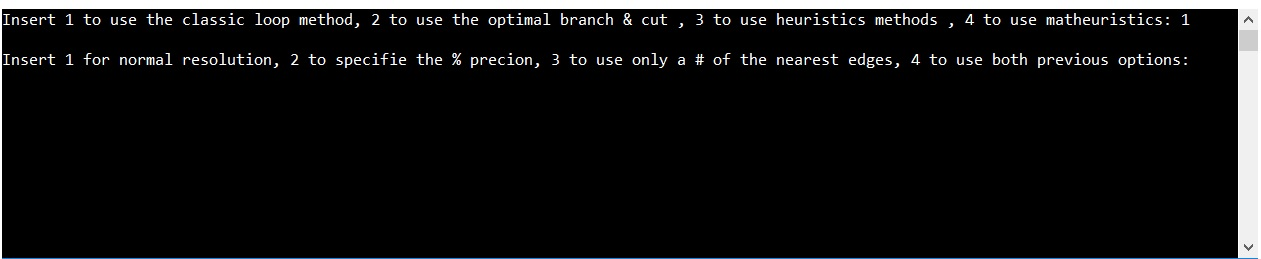
\includegraphics[scale=0.5]{InterfacciaGrafica}  
Figura X: Output 
\end{center}

\vspace{2\baselineskip} 
IMPLEMENTAZIONE FASE EURISTICA 
\vspace{2\baselineskip} 

Nel paragrafo X, si è presentato il metodo BuildModel il cui compito è quello di creare il modello matematico risolubile da Cplex. Durante la presentazione della sua firma, si è lasciato in sospeso la spiegazione del parametro \textit{nEdges} poichè prematura in quel punto della tesi. Il parametro nEdges contiene il valore \textbf{m} fornito in input dall' utente. Qualora l' utente non voglia attivare la prima fase euristica, da programma si assegna a nEdges il valore -1: in questo modo, all' interno di BuildModel, è possibile, attraverso l' utilizzo del costrutto if, creare il modello a seconda se è presente o meno la fase euristica. 

\textbf{[Lo avevi chiamato n il parametro.. ma durante la spiegazione faceva casino con n numero di nodi, quindi ho pensato di rinominare il parametro n in nEdges. Ho modificato anche l' intestazione di BuildModel sopra]}

A livello pratico, per fissare a 0 una variabile, esistono due soluzioni possibili: la prima è, banalmente, non inserire tale variabile nel modello mentre la seconda è fissale il lower bound e l'upper bound di tale variabili a 0. Si è preferito utilizzare questa seconda strategia poichè risulta molto più semplice sia la costruzione del modello(in cui si aggiungono comunque tutte le variabili) sia il ripristino, che precede la fase esatta dell' algoritmo, dell' upper bound al valore 1.
Per poter fissare le variabili congruentemente a quanto detto nel precedente paragrafo, si è realizzato il metodo \textbf{BuildSL} il quale restituisce una lista di vettori di interi, chiamata \textbf{listArray}, in cui il vettore posizionato all' indice $i$ della lista contiene,in ordine crescente in base alla distanza con $i$, gli $n-1$ vertici. In questo modo, per ogni nodo $i$, le variabili che non saranno fissate a 0 saranno quelle associate ai lati [i,k], dove $k$, per costruzione, rappresenta uno dei primi $m$ nodi contenuti nell' i-esimo vettore della lista. 

\begin{lstlisting}

//Init the model's variables
INumVar[] x = new INumVar[(instance.NNodes - 1) * instance.NNodes / 2];

/*
*expr will hold all the expressions that needs to be added to the model
*initially it will be the optimality's functions
*later it will be Ax's rows 
*/
ILinearNumExpr expr = cplex.LinearNumExpr();

for (int i = 0; i < instance.NNodes; i++)
{
    if (nEdges >= 0)
    {
          List<int>[] listArray = BuildSL(instance);

          //Only links (i,i) with i < i are correct
            for (int j = i + 1; j < instance.NNodes; j++)
            {
              //xPos return the correct position where to store the variable corresponding to the actual link (i,i)
              int position = xPos(i, j, instance.NNodes);
            
              if ((listArray[i]).IndexOf(j) < nEdges)
                   x[position] = cplex.NumVar(0, 1, NumVarType.Bool, "x(" + (i + 1) + "," + (j + 1) + ")");
               else
                   x[position] = cplex.NumVar(0, 0, NumVarType.Bool, "x(" + (i + 1) + "," + (j + 1) + ")");
               expr.AddTerm(x[position], Point.Distance(instance.Coord[i], instance.Coord[j], instance.EdgeType));
            }
     }
     else
     {
          //Only links (i,i) with i < i are correct
           for (int j = i + 1; j < instance.NNodes; j++)
           {
               //xPos return the correct position where to store the variable corresponding to the actual link (i,i)
               int position = xPos(i, j, instance.NNodes);
               x[position] = cplex.NumVar(0, 1, NumVarType.Bool, "x(" + (i + 1) + "," + (j + 1) + ")");
               expr.AddTerm(x[position], Point.Distance(instance.Coord[i], instance.Coord[j], instance.EdgeType));
           }
     }
     
     ...
}

\end{lstlisting}


Riportiamo di seguito il codice contenuto nel metodo Loop. Si osserva che una volta che Cplex termina la fase euristica, si è riportato contemporaneamente il valore di EpGap al valore di default e si sono ripristinati gli upper bound di tutte le variabili al valore 1 utilizzando il metodo \textbf{ResetVariables} appartenente alla classe Utility.

\begin{lstlisting}

//COMMENTO!!!!!!!!!!!!!!!!!!!!!!!!!!!!!!!!!!!!!!!!!!!!!
int typeSol = 1;

//epGap is false when EpGap parameter is at default
bool epGap = false;

//allEdges is true when all possible links have their upper bound to 1
bool allEdges = true;

//Setting EpGap if a valid percentage is specified
if (perc >= 0 && perc <= 1)
{
     cplex.SetParam(Cplex.DoubleParam.EpGap, perc);
     epGap = true;
     typeSol = 0;
}

//numb is equal to -1 when all links upper bound are 1
if (numb != -1)
{
     allEdges = false;
     typeSol = 0;
}

//Building the maximum # of links that involves each node
INumVar[] x = Utility.BuildModel(cplex, instance, numb);

//Allocating the correct space to store the optimal solution
//Only links from node i to i with i < i are considered
instance.BestSol = new double[(instance.NNodes - 1) * instance.NNodes / 2];

//Init buffers
int[] relatedComponents = new int[instance.NNodes];
List<ILinearNumExpr> rcExpr = new List<ILinearNumExpr>();
List<int> bufferCoeffRC = new List<int>();

//Temporary variable
double[] linksDistances = new double[(instance.NNodes - 1) * instance.NNodes / 2]; ;

do
{
     //When only one related component is found and ehuristics methods are active they are disabled
      if (rcExpr.Count == 1)
      {
           epGap = false;
           allEdges = true;
           cplex.SetParam(Cplex.DoubleParam.EpGap, 1e-06);
           Utility.ResetVariables(x);
           typeSol = 1;
      }

      //Cplex solves the current model
       cplex.Solve();

       //Initializing the arrays used to eliminate the subtour
       Utility.InitCC(relatedComponents);

       rcExpr = new List<ILinearNumExpr>();
       bufferCoeffRC = new List<int>();

       //Init the StreamWriter for the current solution
        StreamWriter file = new StreamWriter(instance.InputFile + ".dat", false);

        //Storing the optimal value of the objective function
         instance.BestLb = cplex.ObjValue;

         //Blank line
         Console.WriteLine();

         //Printing the optimal solution and the GNUPlot input file
         for (int i = 0; i < instance.NNodes; i++)
         {
              for (int j = i + 1; j < instance.NNodes; j++)
              {

                 //Retriving the correct index position for the current link inside x
                  int position = Utility.xPos(i, j, instance.NNodes);

                  //Reading the optimal solution for the actual link (i,i)
                  linksDistances[position] = cplex.GetValue(x[position]);

                  //Only links in the optimal solution (coefficient = 1) are printed in the GNUPlot file
                  if (linksDistances[position] >= 0.5)
                  {                 
                        //Retriving the correct index position for the current link inside x
                        int position = Utility.xPos(i, j, instance.NNodes);

                        //Reading the optimal solution for the actual link (i,i)
                        linksDistances[position] = cplex.GetValue(x[position]);

                        //Only links in the optimal solution (coefficient = 1) are printed in the GNUPlot file
                        if (linksDistances[position] >= 0.5)
                        {
                            /*
                             *Current GNUPlot format is:
                             *-- previus link --
                             *<Blank line>
                             *Xi Yi <index(i)>
                             *Xj Yj <index(i)>
                             *<Blank line> 
                             *-- next link --
                            */
                            file.WriteLine(instance.Coord[i].X + " " + instance.Coord[i].Y + " " + (i + 1));
                            file.WriteLine(instance.Coord[j].X + " " + instance.Coord[j].Y + " " + (j + 1) + "\n");
                  
                 
                            //Updating the model with the current subtours elimination
                            Utility.UpdateCC(cplex, x, rcExpr, bufferCoeffRC, relatedComponents, i, j);
                  }
               }
          } 

         //Only when more than one related components are found they are added to the model
         if (rcExpr.Count > 1)
         {
                    for (int i = 0; i < rcExpr.Count; i++)
                        cplex.AddLe(rcExpr[i], bufferCoeffRC[i] - 1);
          }

         //GNUPlot input file needs to be closed
         file.Close();

         //Accessing GNUPlot to read the file
         if (Program.VERBOSE >= -1)
            Utility.PrintGNUPlot(process, instance.InputFile, typeSol, instance.BestLb, -1);

          //Blank line
          cplex.Output().WriteLine();

          //Writing the value
          cplex.Output().WriteLine("xOPT = " + instance.BestLb + "\n");

} while (rcExpr.Count > 1 || epGap || !allEdges); //if there is more then one related components the solution is not optimal 

instance.BestSol = linksDistances;
instance.XBest = instance.BestLb;

//Exporting the updated model
if (Program.VERBOSE >= -1)
   cplex.ExportModel(instance.InputFile + ".lp");

//Closing Cplex link
cplex.End();

//Accessing GNUPlot to read the file
if (Program.VERBOSE >= -1)
  Utility.PrintGNUPlot(process, instance.InputFile, typeSol, instance.XBest, -1);
  
\end{lstlisting}



\vspace{2\baselineskip}
CALLBACK
\vspace{2\baselineskip}

In questa sezione esponiamo una tecnica alternativa per l'inserimento delle espressioni di subtour elimination all'interno di un sistema. Ciò che varia rispetto al metodo \textbf{Loop} presentato in precedenza è il \textbf{momento} in cui tali espressioni vengono definite.\\
L'idea è di sfruttare il fatto che Cplex come metodo di risoluzione per i problemi di \textbf{PLI} utilizza la tecnica del \textbf{Branch\&Cut}\footnote{Da ora in avanti sarà abbreviato con la sigla \textbf{B\&C}}. Viene inoltre offerta la possibilità di conoscere la soluzione trovata, sia essa frazionaria o intera, per ogni nodo dell'albero decisione ma soprattuto la possibilità di ampliare il modello matematico come meglio crediamo.\\
Quello che vogliamo fare risulta a questo punto molto chiaro: se alla analisi della soluzione di un nodo sono presenti subtour il modello matematico deve essere modificato per eliminarli.\\
A livello pratico Cplex permette l'implementazione distinta di callback che vengono eseguite nel momento in cui viene trovata una soluzione intera oppure frazionaria\footnote{In informatica una callback è una funzione definita dall'utente che viene eseguita in automatico dal sistema ogniqualvolta scatta un particolare evento.}: nel primo caso è necessario implementare una \textbf{"lazy constraint callback"} mentre nel secondo caso una \textbf{"user cut callback"}. Da notare che in realtà solo soluzioni valide per i criteri di fathoming possono far scattare una callback, ciò non avviene ad esempio se il valore della soluzione di un nodo risulta maggiore rispetto a quello dell'incumbent\footnote{Per incumbent si intende il valore migliore trovato fino a questo momento relativo ad un soluzione accettabile.}.\\
In generale i tagli possono essere definiti \textbf{locali} o \textbf{globali}: mentre i primi hanno validità esclusiva all'interno del sottoalbero avente come radice il nodo per la quale sono stati generati, i secondi hanno validità per tutti i nodi dell'albero decisionale e vengono memorizzati in una struttura globale detta \textbf{pool di tagli}. Cplex inoltre fornisce la possibilità di definire un taglio \textbf{purgeable} o meno: nel primo caso significa che può essere rimosso in un secondo momento poiché ritenuto inefficace. Durante il proseguo della tesi i tagli saranno da considerarsi sempre globali e non purgeable.

\begin{center}
    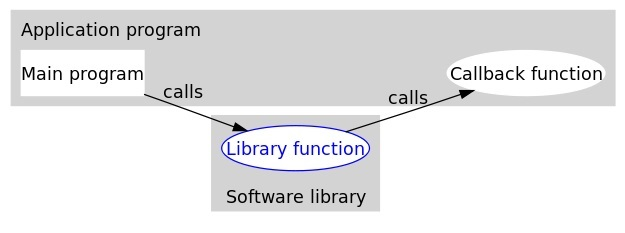
\includegraphics[scale=0.5]{Callback}  
    
    Figura 3: Soluzione frazionaria
\end{center}

Prima di procedere con l'esposizione dei dattagli riguardanti l'implementare di tali procedure, è possibile effettuare le seguenti considerazioni:\\

\begin{itemize}
    \item La soluzione ottima fornita da Cplex risulta per costruzione priva di subtour: non è quindi più necessario, al contrario del metodo \textbf{Loop}, lanciare molteplici risoluzioni. A livello pratico è sufficiente invocare solo una volta il metodo \textbf{Cplex.Solve()}.
    \item Maggiore è il numero di vincoli che andiamo ad inserire, maggiore diventa il tempo di risoluzione per i vari nodi successivi dell'albero decisionale.
    \item Il numero di nodi che forniscono soluzioni frazionarie risulta di molto superiore rispetto a quelli con soluzione intera. Tenendo conto di quanto detto al punto precedente, non è quindi saggio andare ad analizzare tutte le soluzioni frazionarie ma solo una loro minima percentuale. Senza questo accorgimento si andrebbe inevitabilmente ad inserire innumerevoli vincoli superflui per l'ottenenimento della soluzione ottima con conseguenti tempi di risoluzione eccessivamente elevati.
    \item I moderni processori hanno a disposizione molteplici core sia reali che virtuali e quindi sfruttare tecniche di multi-threading. In particolare Cplex permette di settare il numero di thread utilizzabili, in modo tale che ognuno di essi si occupi dalla risoluzione di un nodo dell'albero decisionale: in questo modo, in linea teorica, si drovrebbe ottenere un boost delle prestazioni con conseguente riduzione dei tempi di calcolo. D'altro canto, come per qualsiasi applicazione informatica, l'utilizzo del multi-threading risulta rischioso in quanto l'accesso contemporaneo ai medesimi dati può portare ad una loro inconsistenza. Nel nostro caso può capitare che più callback eseguite contemporaneamente vadano a modificare variabili condivise andando così incontro ad eccezioni o anomalie tali da non garantire più la correttezza della soluzione prodotta da Cplex.\\
    Per evitare queste problematiche, i progettisti di Cplex hanno preferito settare il numero di thread al valore \textbf{1} dopo l' installazione di una callback. \'E quindi nostro compito modificare tale parametro così da renderlo pari al numero di processori virtuali a nostra disposizione e di conseguenza assicurarci che le callback risultino \textbf{thread-safe}. Maggiori dettagli sono riportati nei successivi paragrafi.
\end{itemize}


\vspace{2\baselineskip}
LAZYCONSTRAINT CALLBACK C\#
\vspace{2\baselineskip}


Per poter utilizzare una \textbf{lazy constraint callback} in \textbf{C\#} Cplex fornisce all'interno delle proprie librerie la classe astratta \textbf{LazyConstraintCallback} che a sua volta estende \textbf{ControlCallback}. \'E quindi necessario creare una propria classe che estenda quest'ultima, nel nostro caso è stato deciso di chiamarla \textbf{TSPLazyConsCallback}, in questo modo è necessario definire al suo interno il metodo \textbf{Main} che verrà invocato automaticamente dal sistema ogniqualvolta scatta la callback\footnote{Rocordiamo che tutti i metodi astratti presenti all'interno di una classe astratta devono essere obbligatoriamente definiti da tutte le classi che estendono quest'ultima}.\\
Una volta terminato questo processo l'installazione della callback viene eseguita nel seguente modo:

\begin{lstlisting}

cplex.Use(new TSPLazyConsCallback(...));

\end{lstlisting}

Dove, come al solito, cplex è l'instanza della classe \textbf{Cplex} sulla quale definiamo il modello matematico privo dei vincoli di subtour elimination.\\
Mostriamo ora la firma del costruttore della classe \textbf{TSPLazyConsCallback} riportando una breve descrizione dei parametri di ingresso:

\begin{lstlisting}

public TSPLazyConsCallback(Cplex cplex, INumVar[] z, Instance instance, Process process, bool BlockPrint)

\end{lstlisting}

\begin{itemize}
    \item \textbf{cplex}: necessario per l'individuazione dei vincoli di subtour elimination, contiene i dati del modello matematico utilizzato;
    \item \textbf{z}: identico al punto precedente, contiene i riferimenti alla variabili del modello matematico;
    \item \textbf{instance}: necessario nel caso in cui si desideri stampare attraverso GNUPlot le soluzioni intere che hanno fatto scattare la callback;
    \item \textbf{process}: identico al punto precedente;
    \item \textbf{BlockPrint}: è il parametro booleano che determina se procedere o meno con le stampe delle soluzioni intere (se \textbf{true} si procede con la stampa);
\end{itemize}

Come accennato nel paragrafo precedente, l'installazione di una callback setta automaticamente il numero di thread ad uno. Per modificare tale valore, ponendolo pari al numero logico di cores messi a disposizione dal processo in uso, è sufficiente eseguire la seguente riga di codice:

\begin{lstlisting}

cplex.SetParam(Cplex.Param.Threads, cplex.GetNumCores());

\end{lstlisting}

Come sarà possibile vedere più avanti, la tecnica da noi utilizzata per l'individuazione di subtour risulta thread-safe in quanto non vengono utilizzate variabili condivise da più threads se non nella sola modalità di lettura. L'aggiunta di eventuali tagli, d'altro canto, viene gestita in modo automatico da Cplex assicurandoci, anche in questo caso, una procedura thread-safe. Un discorso apparte deve invece essere fatto nel caso in cui la variabile \textbf{BlockPrint} descritta in precedenza sia stata posta a \textbf{true}. Come era logico aspettarsi, abbiamo verificato che spesso la procedura di stampa attraverso GNUPlot di una qualsiasi soluzione richiede un tempo di esecuzione maggiore rispetto la frequenza con cui le callback sono effettuate. Ricordando inoltre che, il metodo da noi utilizzato per comunicare a GNUPlot le coordinate cartesiane dei punti del grafo cartesiano prevede la scrittura di queste ultime in un apposito file di testo, è stato necessario individuare un modo per evitare problemi riguardanti il multi-threading: utilizzare sempre lo stesso file di testo causa infatti errori nella stampa dei grafi, in particolare la lettura delle coordinate da parte di GNUPlot risulta troppo lenta e durante questo processo più thread rischiano di modificare il file con le proprie coordinate.\\
Per evitare questo problema è stato quindi necessario stampare le coordinate prodotte dai vari nodi dell'albero decisionale in differenti files. A tal proposito la tecnica da noi scelta è stata quella di inserire nel nome di questi ultimi anche l'id numerico del nodo a loro associato che viene fornito dirretamente da Cplex:


\begin{lstlisting}

string nodeId = GetNodeId().ToString();

...

string fileName = instance.InputFile + "_" + nodeId;

\end{lstlisting}

La funzione \textbf{GetNodeId} risulta disponibile in quanto ereditata dalla classe \textbf{ControlCallback}.\\
Dopo i dovuti chiarimenti riguardanti il multi-threading passiamo ora a descrivere nei dettagli come è stata realizzato il metodo Main della classe TSPLazyConsCallback. Prima di tutto per verificare l'eventuale presenza di subtour bisogna naturalmente accedere alla soluzione fornita per il nodo dell'albero decisionale in questione: a tal fine si possono utilizzare i metodi \textbf{GetValues} e \textbf{GetValue}, ereditati entrambi dalla classe ControlCallback, che ricevono in input rispettivamente un vettore di riferimenti per variabili del modello matematico e un singolo riferimento ad una variabile di quest'ultimo. Dopo pochi test ci si accorge immediatamente che invocare più volte il metodo \textbf{GetValue}, ad esempio dentro un ciclo for, risulta molto più oneroso in termini temporali rispetto una singola evocazione del metodo \textbf{GetValues}: si può quindi dedurre che è molto più dispendioso effettuare multiplici accessi all'interfaccia fornita da Cplex rispetto alla quantità di dati che ad essa richiediamo.\\
Per quanto appena detto la nostra scelta è ricaduta nel metodo \textbf{GetValues} che restituisce un vettori di \textbf{double} contenente il valore dell variabili (il cui riferimento è ricevuto come ingresso) nella soluzione corrente del modello matematico. Da notare che anche in questo caso anche se ci aspettiamo tutti valori interi, in particolare pari a 0 oppure 1, è possibile che ci siano in realtà discostamenti infinitesimi pertanto quando controlliamo il valore di una variabile verifichiamo semplicemente se è maggiore o minore del valore 0,5.\\
I metodi utilizzati per l'individuazione di eventuali subtour e la eventuale stampa del grafo attraverso GNUPlot sono identici a quelli utilizzati per il metodo \textbf{Loop} pertanto non sono qui riportarti.\\
Una volta ottenute tutte le informazioni riguardanti i subtour, al contrario di quanto viene fatto nel metodo Loop non è richiesto di ampliare direttamente il modello con nuovi vincoli ma, come era già stato accennato in precedenza, deve essere popolato il pool di tagli associato al modello matematico:

\begin{lstlisting}

IRange[] cuts = new IRange[ccExprLC.Count];

//if cuts.Length is 1 the graph has only one tour then cuts aren't needed
if (cuts.Length > 1)
{
    for (int i = 0; i < cuts.Length; i++)
    {
        cuts[i] = cplex.Le(ccExprLC[i], bufferCoeffCCLC[i] - 1);
        Add(cuts[i], 1);
    }
}

\end{lstlisting}

Dove:

\begin{itemize}
    \item \textbf{cuts}: è un vettore di \textbf{IRange} che sono la struttura di dati base fornita da Cplex per memorizzare espressioni lineari;
    \item \textbf{ccExprLC[i]}: analogamente per quanto avviene nel metodo Loop, contiene i dati delle variabili dell'i-esimo taglio memorizzati come \textbf{ILinearNumExpr} (struttura dati fornita da Cplex);
    \item \textbf{bufferCoeffCCLC[i]}: analogamente per quanto avviene nel metodo Loop, contiene il numero di variabili che definiscono l'i-esimo taglio;
    \item \textbf{cplex.Le}: è la funzione definita da Cplex che restituisce una espressione lineare che impone le variabili, ricevute come primo parametro, minori oppure uguali del secondo parametro ricevuto;
    \item \textbf{Add}: è la funzione eraditata dalla classe \textbf{LazyConstraintCallback} che permette di aggiungere un taglio \textbf{globale}. Come parametri riceve quindi il taglio stesso ed un valore intero che indica a Cplex come debba gestire quest'ultimo:
    \begin{itemize}
        \item \textbf{0}: il taglio è aggiunto al pool in maniera permanente;
        \item \textbf{1}: il taglio è definito come \textbf{purgeable} quindi eliminabile nel caso in cui non risulti più efficiente;
        \item \textbf{2}: il taglio viene trattato come se fosse stato generato da Cplex, quindi ad esempio prima di essere aggiunto al pool viene analizzata la sua efficacia e di conseguenza l'operazione va quindi a buon fino o meno;
    \end{itemize}

\end{itemize}


\vspace{2\baselineskip}
CONCORDE
\vspace{2\baselineskip}

L'utilizzo di una \textbf{user cut callback} risulta molto più complicato rispetto a quanto appena visto per la \textbf{lazy constraint callback}: dato che tali callback scattano nel momento in cui viene trovata una soluzione frazionaria, l'individuazione di eventuali subtour non può essere eseguita con le tecniche esposte fino ad ora.\\
Per effetturare tale operazione si necessita di un separatore che, ricevendo in ingresso la soluzione x* con almeno una componente frazionaria, fornisca in uscita un insieme $S\subsetneq{V}$, $|S|\geq{2}$ tale per cui:

\begin{equation}\label{eq:concorde1}
\displaystyle{\sum_{\left ( i,j \right )\in E\left ( S \right )} x_{i,j}^{*}\nleqslant \left | \widehat{S} \right |-1}
\end{equation}

Tale sottoinsieme non è facilmente individuabile come nel caso di soluzione intere in cui era sufficiente individuare le componenti connesse. Per esempio in Figura 3 si è riportato il supporto di una soluzione x* frazionaria ove i lati colorati di rosso, blu e grigio indicano che la corrispondente variabile assumme rispettivamente i valori 1, 0.5 , 1.5.

\begin{center}
    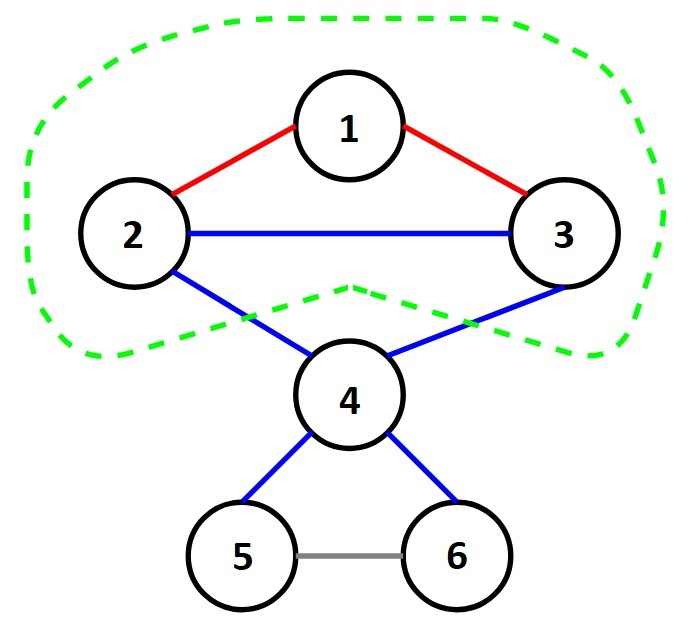
\includegraphics[scale=0.5]{SoluzioneFrazionaria}  
    
    Figura 3: Soluzione frazionaria
\end{center}

Tale grafo risulta connesso; tuttavia è presente un sottoinsieme S = {1,2,3} per cui vale \eqref{eq:concorde1}.\\
Una seconda formulazione equivalente alla \eqref{eq:concorde1} risulta essere la seguente:

\begin{equation}\label{eq:concorde2}
\displaystyle{\sum_{\left ( i,j \right )\in \delta \left ( S \right )} x_{i,j}^{*}\ngeqslant 2}
\end{equation}

Si osserva che il primo membro di \eqref{eq:concorde2} può essere visto come la capacità di una sezione di una rete di flusso se si interpretano le x* come le capacità della rete.
E' possibile calcolare una sezione di capacità minima risolvendo un problema di max flow che sappiamo essere di programmazione lineare e quindi risolubile attraverso un algoritmo polinomiale.\\
Poichè però la sezione di capacità minima dipende dal nodo sorgente \textit{s} e dal nodo di destinazione \textit{t}, si devono in realtà risolvere \textbf{n-1} problemi di max flow: per tale ragione è stato preferito utilizzare una porzione del software \textbf{Concorde} che offre, attraverso le proprie librerie, la possibilità di risolvere tale problema con tempi di esecuzione molto brevi ed allo stesso tempo di alleggerire il nostro carico di lavoro che in ogni caso non avrebbe prodotto risultati migliori.\\
Concorde è un software, sviluppano in linguaggio \textbf{C} da David Applegate, Robert E. Bixby, Vašek Chvátal, e William J. Cook, specializzato nella risoluzione ottimizzata di istanze del problema del commesso viaggiatore. Per fini accademici la distribuzione e l'utilizzo è fornita in modo gratuito e le librerei possono essere scaricate direttamente dal seguente indirizzo:
\begin{center}
\href{http://www.math.uwaterloo.ca/tsp/concorde/downloads/downloads.htm}{http://www.math.uwaterloo.ca/tsp/concorde/downloads/downloads.htm}
\end{center}

Come accennato poco fa il linguaggio utilizzato da Concorde non è \textbf{C\#} bensì \textbf{C} pertanto una implementazione diretta del software non è possibile. La soluzione da noi adottata è la seguente: abbiamo creato un nuovo progetto Visual Studio in linguaggio \textbf{C/C++} ed al suo interno abbiamo creato un codice che soddisfacesse unicamente alla funzionalità ambedue i tipi di callback proposti interfacciandosi alle librerie di Concorde per trovare i vincoli di subtour elimination ed aggiungerli al modello matematico. Successivamente il tutto è stato impachettato all'interno di una \textbf{DLL} compatibile con il linguaggio \textbf{C\#}. Il processo di creazione della DLL è stato spiegato nel seguente paragrafo LINK!!!!!!!!!!!!!!!!!!!!, d'ora in avanti quindi ci focalizzeremo unicamente nel contenuto della libreria dinamica da noi creata.\\

Per poter utilizzare Concorde in ambiente Windows è necessario importare ogni singolo file .c e .h che appartiene alla distribuzione: nel nostro caso però solo una minima parte delle sue funzionalità è di nostro interesse e pertanto solamente i seguenti file sono stati da noi utilizzati:


\begin{itemize}
    \item \textbf{allocrus.c}
    \item \textbf{connect.c}
    \item \textbf{cut\_st.c}
    \item \textbf{mincut.c}
    \item \textbf{shrink.c}
    \item \textbf{sortrus.c}
    \item \textbf{urandom.c}
    \item \textbf{cut.h}
    \item \textbf{machdefs.h}
    \item \textbf{macrorus.h}
    \item \textbf{util.h}
    \item \textbf{end}
\end{itemize}

Dove affinché il programma compili correttamente, è necessario effettuare le seguenti modifiche:

\begin{itemize}
    \item All'interno dei file \textbf{allocrus.c} e \textbf{util.h} è necessario importare tramite il comando \textbf{import} l'header \textbf{malloc.h}.
    \item All' interno del file \textbf{machdefs.h} è necessario eliminare l'inclusione di \textbf{config.h}.
\end{itemize}

\vspace{2\baselineskip}
LAZYCONSTRAINTCALLBACK IN C
\vspace{2\baselineskip}


In questa mostreremo solamente i dettagli per l'installazione e l'utilizzo delle \textbf{lazyconstraint callback} in linguaggio \textbf{C} in quanto un discorso più ampio è stato precedentemente in LINK!!!!!!!!!.
L'installazione di questo tipo di callback avviene attraverso l'invocazione della routine \textbf{CPXsetlazyconstraintcallbackfunc} la cui firma è:

\begin{lstlisting}

CPXsetlazyconstraintcallbackfunc(CPXENVptr env,int(*)(CALLBACK\_CUT\_ARGS) lazyconcallback, void * cbhandle)

\end{lstlisting}

Dove:

\begin{itemize}
    \item \textbf{env}: Espressione contenente una combinazione lineare delle variabili del vincolo; SIAMO SICURI!!!!???!??!
    \item \textbf{lazyconcallback}: Rappresenta il nome, attribuito dal programmatore esterno, della funzione che viene invocata da Cplex qualora la soluzione del rilassamento continuo di un nodo abbia valore intero ed inferiore all'incumbent. Nel nostro caso il nome assunto è \textbf{myLazyCallBack};
    \item \textbf{cbhandle}: Puntatore ad una struttura dati passata dall'utente contenente le informazioni che devono essere visibili all'interno della callback \textit{myLazyCallBack}. Come parametro si è passato il puntatore all'istanza;
\end{itemize}

In modo del tutto analogo a quanto fatto per \textbf{C\#}, per impostare il numero di thread pari ai core virtuali offerti dalla macchina in utilizzo si sono utilizzati i metodi \textbf{CPXsetintparam} e \textbf{CPXgetnumcores}:

\begin{lstlisting}

CPXgetnumcores(env, int * nCore);
CPXsetintparam(env, CPXPARAM\_Threads, nCore);


\end{lstlisting}

Passiamo ora a descrivere la funzione \textit{myLazyCallBack} che identifica i subtour ed aggiunge i relativi vincoli al modello, ricordando che la sua firma deve rispettare specifici parametri definiti da Cplex stesso\footnote{Essendo tali funzioni invocate automaticamente da Cplex i tipi di parametri che esse ricevono sono stati definiti a priori e non risultano modificabili}:

\begin{lstlisting}

static int CPXPUBLIC myLazyCallBack(CPXCENVptr env, void *cbdata, int wherefrom, void *cbhandle, int *useraction\_p)

\end{lstlisting}

Dove:

\begin{itemize}
    \item \textbf{env}: rappresenta l’istanza dell’ enviroment con il quale stiamo lavorando. DIVERSO DA SOPRA!!!!!!!!
    \item \textbf{cbdata}: come accennato poco fa questo parametro è quello specificato dall'utente durante l'installazione della callback, non essendo noto a priori il tipo di dato che l'utente desidera ricevere si utilizza \textbf{void};
    \item \textbf{wherefrom}: definisce da che punto del \textit{B\&C} è stata invocata la funzione, ai fini pratici tale parametro, per la lazy callback è risultato irrilevante;
    \item \textbf{cbhandle}: puntatore a dati privati utilizzato da Cplex;
    \item \textbf{useraction\_p}: puntatore ad un intero utilizzato dall'utente per comunicare a Cplex diverse informazioni. Tale parametro può assumere i seguenti tre valori:
    \begin{itemize}
    \item \textbf{0}: avente come costante simbolica CPX\_CALLBACK\_DEFAULT comunica a Cplex che fino a quel punto la callback non ha aggiunto tagli al modello;
    \item \textbf{1}: avente come costante simbolica CPX\_CALLBACK\_FAI impone a Cplex di uscire dall'ottimizzazione;
    \item \textbf{2}: avente come costante simbolica CPX\_CALLBACK\_SET comunica a Cplex che sono stati aggiunti tagli;
    \end{itemize}

\end{itemize}

La prima operazione da compiere consiste nell effettuare un cast al puntatore \textbf{cbhandle} il cui tipo è noto solo al programmatore che ha installato la callback: nel nostro caso il puntatore è di tipo \textbf{instance} per cui:


\begin{lstlisting}

instance *inst = (instance*)cbhandle;

\end{lstlisting}

Successivamente è necessario assegnare al parametro \textbf{*useraction\_p} il valore \textbf{CPX\_CALLBACK\_DEFAULT}.

Per ottenere la soluzione del rilassamento continuo è necessario utilizzare il metodo \textbf{CPXgetcallbacknodex} avente come intestazione:

\begin{lstlisting}

int CPXgetcallbacknodex(CPXCENVptr env, void * cbdata, int wherefrom, double * x, int begin, int end) 

\end{lstlisting}

Dove:

\begin{itemize}
    \item Per quanto riguarda env, cbdata, wherefrom vale la descrizione vista per il metodo myLazyCallBack;
    \item \textbf{x}: array che al termine del metodo conterrà la soluzione intera del rilassamento continuo;
    \item \textbf{begin}: indica l’indice della prima variabile di cui si vuole conoscere il valore;
    \item \textbf{end}: indica l’indice dell’ultima variabile di cui si vuole conoscere il valore;
\end{itemize}

Nel nostro caso dato che vogliamo conoscere tutte le variabili, assegniamo i valori \textbf{$0$} e \textbf{$[n*(n-1)/2] – 1$} rispettivamente ai parametri \textbf{begin} ed \textbf{end}.

All'atto dell'invocazione del metodo \textit{CPXgetcallbacknodex} non viene passato come parametro l'array \textbf{bestLb} contenuto in \textit{inst} ma viene creato un opportuno array chiamato \textbf{xstar}:

\begin{lstlisting}

double *xstar = (double*)malloc(inst->nCols * sizeof(double));

\end{lstlisting}

Questa operazione risulta necessaria al fine di realizzare un codice che risulti thread-safety: poiché \textit{inst} è un puntatore accessibile da tutti i thread esiste il rischio di accessi multipli sia in modalità di lettura popolando così \textit{bestLb} con valori appartenti a soluzioni differenti.
A questo punto entra in gioco Concorde per l'individuazione e l'introduzione dei vincoli di subtour elination, dato che il metodo da utilizzare è il medesimo che vedremo per le \textit{usercut callback} rimandiamo al paragrafo seguente per maggiori dettagli.
Una volta completato tale passaggio non rimane altro che impostare il parametro \textbf{*useraction\_p} al valore \textbf{CPX\_CALLBACK\_SET} al fine di comunicare a Cplex che sono stati aggiunti tagli.

\vspace{2\baselineskip}
USERCUT CALLBACK IN C
\vspace{2\baselineskip}

Come già anticipato nei precedenti paragrafi questo tipo di callback sono utilizzate per gestire soluzioni frazionarie ottenute per i vari nodidell'albero decisionale durante una risoluzione di tipo \textit{B\&C} per problemi di programmazione lineare da parte di Cplex. A livello concettuale sono del tutto simili a quanto visto nel paragrafo precedente per le \textit{lazy callback} in linguaggio \textbf{C}, è raccomandata una lettura del paragrafo precedente a loro dedicato in quanto di seguito saranno esposti estensivamente solamente i dettagli riguardanti la gestione dei tagli.\footnote{Notiamo in realtà che l'implementazione delle \textit{usercut callback} avviene sempre in concomitanza all'implementazione delle \textit{lazy callback} per tanto il settaggio del numero di thread è necessario solamente una volta}.

L'installazione delle callback avviene tramite la funzione \textbf{CPXsetusercutcallbackfunc}:

\begin{lstlisting}

int CPXsetusercutcallbackfunc (CPXENVptr env, int(*)(CALLBACK\_CUT\_ARGS) lazyconcallback, void * cbhandle)

\end{lstlisting}

La funzione invocata da Cplex in corrispondenza di una soluzione frazionaria è stata da noi chiamata \textbf{myUserCutCallBack} la cui firma, che anche in questo caso viene imposta dai progettisti di Cplex, risulta essere:

\begin{lstlisting}

int CPXPUBLIC myUserCutCallBack(CPXCENVptr env, void *cbdata, int wherefrom, void *cbhandle, int *useraction\_p)

\end{lstlisting}

Cplex, una volta calcolata una soluzione frazionara, genera in automatico dei propri tagli\footnote{Ad esempio taglio di \textit{Gomory}}. Quando il parametro \textit{wherefrom} risulta pari a \textbf{CPX\_CALLBACK\_MIP\_CUT\_LAST} significa che l'iterazione successiva da parte di Cplex consisterebbe nell'operazione di branching sul nodo in questione: solo in questa condizione risulta conveniente generare i propri vincoli caratteristici del problema che si sta risolvendo. Qualora il parametro \textit{wherefrom} assuma invece altri valori, si effettua una semplice \textbf{return 0} senza eseguire alcuna operazione, altrimenti come già discusso per le lazy, è necessario recuperare il puntate all’istanza.
Riprendendo quanto detto nel paragrafo LINK PARAGRAFO CALLBACK||||| è sconsigliato aggiungere \textit{manualmente} ad ogni nodo dell’albero decisionale dei tagli in quanto il loro numero complessivo risulterebbe troppo elevato andando quindi a \textbf{peggiorare} le prestazioni di Cplex. Per tale ragione, dopo alcuni test e secondo le linee guida discusse durante il corso, si è deciso che solamente con una probabilità del \textbf{$10\%$} la \textit{usercut callback} da noi definita entra in gioco. Dato che l'id numerico assegnato ai nodi dell'albero decisionale, ottenuto attraverso al funzione \textbf{CPXgetcallbacknodeinfo}, non ha alcuna relazione diretta alla probabilità che venga generata una soluzione intera oppure frazionaria, è sufficiente effettuare una operazione di modulo dieci a tale valore: nel caso in cui il risultato sia pari a zero si procede con il calcolo dei tagli. Successivamente, invocando la nota funzione \textbf{CPXgetcallbacknodex} si ottiene la soluzione frazionaria. Prima di procedere con la parte principale di questo metodo, per ragioni di chiarezza riportiamo il codice che esegue quanto finora descritto:


\begin{lstlisting}

*useraction\_p = CPX\_CALLBACK\_DEFAULT;
    
int nodecount = 0;
CPXgetcallbacknodeinfo(env, cbdata, wherefrom, 0, CPX\_CALLBACK\_INFO\_NODE\_DEPTH, &nodecount);
    
if (wherefrom == CPX\_CALLBACK\_MIP\_CUT\_LAST)
{
    instance *inst = (instance*)cbhandle;
        
    double *xstar = (double*)malloc(inst->nCols * sizeof(double));

     if ((nodecount % 10) != 0)
        return 0;

    if (CPXgetcallbacknodex(env, cbdata, wherefrom, xstar, 0, inst->nCols - 1))
    {
        free(comps);
        free(compscount);
        free(xstar);
        free(elist);
        return 1; 
    }
}

\end{lstlisting}


Da questo momento inizieremo ad utilizzare le funzionalità offerta da \textit{Concorde}, tutte le funzioni il cuo nome inizia con la sigla \textbf{"CC"} sono importate da quest'ultimo.
L'aggiunta di eventuali vincoli di \textit{subtour elimination} avviene tramite l'invocazione in un primo momento della funzione \textbf{CCcut\_connect\_components} la quale identifica le componenti connesse della soluzione ricevuta come parametro indipendentemente dal fatto che sia intera o frazionaria.

Di seguito sono riportati nel dettaglio tutti i parametri che tale funzione vuole ricevere in ingresso, si osserva che mentre i primi 4 costituiscono l'effettivo input della funzione i rimanenti 3 sono in realtà settata al suo interno e quindi possono essere visti come parametri di output:

\begin{itemize}
    \item \textbf{ncount}: rappresenta il numero di nodi del grafo;
    \item \textbf{econut}: rappresenta il numero di lati del grafo, ossia ncount*(ncount-1)/2;
    \item \textbf{*elist}: vettore di dimensione $2*econut$, contiene al suo interno tutti i lati del grafo caratterizzati dai nodi sul quale esso incide memorizzati in locazioni consecutive dell’array, è stato da noi realizzato nel seguente modo:
    
    \begin{lstlisting}
    
    int loader = 0;
    for (int i = 0; i < inst->nNodes;  i++)
    {
        for (int j = i + 1; j < inst->nNodes;  j++) 
        {
            elist[loader++] = i;
            elist[loader++] = j;
        }
    }
    
    \end{lstlisting}
    
    \item \textbf{*x}: soluzione per la quale si desiderano individuare le componenti connesse;
    \item \textbf{*ncomp}: rappresenta il numero di componenti connesse;
    \item \textbf{**compscount}: vettore di vettori contenenti il numero di nodi per ciascuna componente connessa, è strutturato in modo che compscount[i] contenga il numero di nodi presente nell’i-esima componente connessa;
    \item \textbf{**comps}: vettore di vettori contenenti gli indici dei nodi presenti all'interno delle componenti;
\end{itemize}

Nonostante non risulti necessario, al fine di rendere il codice maggiormente leggibile, si è deciso di assegnare sia alle variabili che ai puntatori il medesimo nome che assumono all’interno di \textit{CCcut\_connect\_components}.

\begin{lstlisting}

int *compscount = (int*)malloc(inst->nMaxCuts * sizeof(int));
int *comps = (int*)malloc(inst->nNodes * sizeof(int));
int nLati = ((inst->nNodes - 1)*inst->nNodes / 2);
int *elist = (int*)malloc((nLati * 2) * sizeof(int));
int ncomp; 

\end{lstlisting}

La chiamata alla funzione risulta quindi essere:

\begin{lstlisting}
if (CCcut\_connect\_components(inst->nNodes, nLati, elist, xstar, &ncomp, &compscount, &comps))
    printError(" error in CCcut\_connect\_components() inside fractcutusercallback");
\end{lstlisting}

Al suo termine, in modo del tutto trasparente, otteniamo le tre variabili \textbf{ncomp}, \textbf{compscount} e \textbf{comps} che forniscono tutte le informazioni necessarie all'aggiunta dei tagli all'interno dell'apposito pool fornito da Cplex.
Completiamo quest'ultima operazione tramite la routine fornita da Cplex \textbf{CPXcutcallbackadd} la cui firma è:

\begin{lstlisting}

CPXcutcallbackadd(CPXCENVptr env,void * cbdata,int  wherefrom,int  nzcnt, double  rhs,int sense,int cutind,double const *  cutval, int purgeable);

\end{lstlisting}

Dove:

\begin{itemize}
    \item \textbf{env,cbdata,wherefrom}: parametri noti già discussi nella callback myLazyCallback;
    \item \textbf{nzcnt}: numero di coefficienti diversi da zero del vincolo;
    \item \textbf{rhs}: definisce il termine noto del vincolo;
    \item \textbf{sense}: può assumere i seguenti valori:
    
    \begin{itemize}
    \item \textbf{cutind}: array di \textit{nzcnt} elementi contenenti gli indici delle variabili presenti nel vincolo;
    \item \textbf{cutval}: array di \textit{nzcnt} elementi contenenti i corrispondenti valori dei coefficienti;
    \item \textbf{purgeable}: valore intero che specifica come Cplex deve trattare il taglio:
    
        \begin{itemize}
        \item \textbf{CPX\_USECUT\_FORCE}: il taglio una volta aggiunto al rilassamento non può essere più rimosso;
        \item \textbf{CPX\_USECUT\_PURGE}: il taglio è aggiunto al rilassamento ma può essere eliminato in un secondo momento se giudicato inefficiente;
        \item \textbf{CPX\_USECUT\_FILTER}: il taglio deve essere trattato come se generato da Cplex il quale prima di aggiungerlo al rilassamento lo analizza e può quindi decidere di abortire l'operazione di aggiunta.
        nel rilassamento(per esempio è già presente un taglio più efficiente);
        \end{itemize}
    \end{itemize}
\end{itemize}

Per aggiungere un taglio per ogni componente connessa è necessario popolare i vettori \textbf{cutval}, \textbf{cutind} e la variabile \textbf{nzcnt} opportunamente sfruttando le informazioni fornite da \textit{Concorde}. Per stabilire quali nodi appartengono alla t-esima componente connessa si sono dichiarate due variabili intere \textbf{k1} e \textbf{k2} che contengono sistematicamente l'indice del \textbf{primo} e dell'\textbf{ultimo} nodo tra quelli appartenenti alla t-esima componente connessa memorizzata in \textit{comps}. Si osserva che \textit{k2} è inizializzato al valore \textbf{$-1$} in quanto gli indici di un qualsiasi vettore partono da $0$.

\begin{lstlisting}

    if (ncomp > 1)
        {
            int k1 = 0;
            int k2 = -1;

            for (int c = 0; c < ncomp; c++)
            {
                int dimIndexValue = compscount[c] * (compscount[c] - 1) / 2; 
                int *cutind = (int*)malloc(dimIndexValue * sizeof(int));
                double *cutval = (double*)malloc(dimIndexValue * sizeof(double));
                int nzcnt = 0;

                
                k2 += compscount[c];

                for (int i = k1; i < k2; i++)
                {
                    for (int j = i + 1; j <= k2; j++)
                    {
                        cutval[nzcnt] = 1.0;
                        cutind[nzcnt] = xPos(comps[i], comps[j], inst);
                        nzcnt++;
                    }
                }

                k1 = k2 + 1;
                
                CPXcutcallbackadd(env, cbdata, wherefrom, nzcnt, compscount[c] - 1, 'L', cutind, cutval, CPX\_USECUT\_FORCE);

                *useraction\_p = CPX\_CALLBACK\_SET; 
                free(cutind);
                free(cutval);
            }

            free(elist);
            free(comps);
            free(compscount);
            free(xstar);


            return 0;
        }

\end{lstlisting}

Nel caso in cui la soluzione presenti una sola componente connessa, come in Fig. X, invocando la funzione \textbf{CCcut\_violated\_cuts} di \textit{Concorde} è possibile individuare gli insiemi $S$ che soddisfino la disuguaglianza \eqref{eq:concorde2}: noto $S$ risulta poi banale inserire il relativo vincolo di subtour. In particolare \textit{CCcut\_violated\_cuts} è una funzione in grado di individuare sezioni di capacità inferiori ad una certa soglia. Descriviamo quindi i 7 parametri che tale funzione riceve in input:

\begin{itemize}
    \item \textbf{int ncount}, \textbf{int ecount}, \textbf{int *elist}: il loro significato è già stato descritto per la funzione \textit{CCcut\_connect\_components};
    \item \textbf{dlen}: vettore contenente la capacità di ogni lato;
    \item \textbf{cutoff}:[Questo è il termine noto della disequazione f2, non ho capito perchè devo togliere a 2 un EPSILON, così è scritto nel pdf condiviso dal prof che si chiama         RO2\_TSPutilities]
    \item \textbf{(*(doit\_fn)(double, int, int *, void *) }: è una funzione creata da noi che risulta essere una vera e propria callback: ogniqualvolta \textit{Concorde} individua un insieme $S$ cercato tale funzione viene invocata. Al suo interno, grazie ai parametri forniti\footnote{Maggiori dettagli riguardo i quattro parametri di ingresso saranno forniti a breve durante la descrizione di come l'implementazione di tale funzione è stata da noi realizzata.} è nostro compito procedere all'ampliamento del pool di tagli di \textit{Cplex}.
    \item \textbf{pass\_param}: puntatore ad una struttura dati contenente variabili e puntatori che devono essere accessibili all’interno della callback;
\end{itemize}

Nel nostro caso l'invocazione di tale metodo avviene nel seguente modo:

\begin{lstlisting}

CCcut_violated_cuts(inst->nNodes, inst->nCols, elist, xstar, 2.0 - cutThreshold, doitFuncConcorde, (void*)&in)

\end{lstlisting}

Dove occorre solamente far notare che la funzione callback da noi definita prende il nome \textbf{doitFuncConcorde} mentre l'ultimo parametro è una \textbf{struct} da noi creata contenente al suo interno tutte le informazioni occorrenti per invocare il metodo \textbf{CPXcutcallbackadd}, descritto in precedenza, all'interno della callback.

\begin{lstlisting}

typedef struct 
{
    instance *inst;
    CPXCENVptr env;
    void *cbdata;
    int wherefrom;
    int *useraction\_p;
} inputCC;

\end{lstlisting}

Per concludere questo paragrafo non rimane altro che parlare più in dettagli riguardo la realizzazione della callback \textbf{doitFuncConcorde}, per prima cosa forniamo la sua firma:

\begin{lstlisting}

int doitFuncConcorde(double cutValue, int cutcount, int *cut, void *inParam)

\end{lstlisting}

Dove:

\begin{itemize}
    \item \textbf{cutValue}: rappresenta il valore del taglio;
    \item \textbf{cutcount}: rappresenta il numero dei nodi;
    \item \textbf{cut}: array contenente l'indice associato ai nodi;
    \item \textbf{inParam}: struttura dati appena descritta;
\end{itemize}

Dopo aver effettuato la classica operazione di recupero del puntatore alla struttura dati fornita in ingresso alla callback

\begin{lstlisting}

inputCC *in = (inputCC*)inParam;

\end{lstlisting}

possiamo procedere con l'aggiunta del taglio  attraverso \textit{CPXcutcallbackadd}: si sono così definiti due array di interi \textbf{cutind} e \textbf{cutval} contenenti rispettivamente gli indici delle variabili che costituiscono il taglio ed il relativo coefficiente. Si è inoltre dichiarata una variabile intera \textbf{nzcnt} che contiene il numero di variabili caratterizzanti il taglio:

\begin{lstlisting}

int dimIndexValue = inst->nNodes * (inst->nNodes - 1) / 2;
int *cutind = (int*)malloc(dimIndexValue * sizeof(int));
double *cutval = (double*)malloc(dimIndexValue * sizeof(double));
int nzcnt = 0;

    for (int i = 0; i < cutcount - 1; i++)
    {
        for (int j = i + 1; j <= cutcount - 1; j++)
        {
            int n1 = cut[i];
            int n2 = cut[j];
            !!!!!!!!!!!!!!!!!!!!!!!!!!!!!!!!!!!!!!!!!!!!!!!!!!!!!!!!!!!!!!!!!!!!!!!!!!!!!!!!!!!!!!!!!!!!!!!!!!!!!!!!!!
            METTI QUA IL COMMENTO A xPos che avevi fatto... il codice va commentato !!!!!!!!!!!!!!!!!!!!!!!!!!!!!!!!!!
            !!!!!!!!!!!!!!!!!!!!!!!!!!!!!!!!!!!!!!!!!!!!!!!!!!!!!!!!!!!!!!!!!!!!!!!!!!!!!!!!!!!!!!!!!!!!!!!!!!!!!!!!!!
            cutind[nzcnt] = xPos(n1, n2, inst);
            cutval[nzcnt] = 1.0;
            nzcnt++;
        }
    }
CPXcutcallbackadd(in->env, in->cbdata, in->wherefrom, nzcnt, cutcount - 1, 'L', cutind, cutval, CPX\_USECUT\_FORCE);

*in->useraction\_p = CPX\_CALLBACK\_SET;

free(cutind);
free(cutval);

return 0;

\end{lstlisting}



\vspace{2\baselineskip}
INTRODUZIONE EURISTICI
\vspace{2\baselineskip}

Nei paragrafi precedenti sono stati presentati metodi che garantiscono di risolvere una generica istanza del problema del commesso viaggiatore in modo esatto, ovvero restituendo sempre un ottimo globale come soluzione.
L'applicazione di metodi esatti non è sempre possibile: ciò non è dovuto solamente alla complessità intrinseca del problema, che come noto è NP-hard, ma anche dal tempo che l' algoritmo dispone per calcolare una soluzione. 
Per tali ragioni, nelle applicazioni reali, spesso l' unica strada percorribile è ricorrere a metodi che permettono di trovare delle "buone" soluzioni senza garantire la loro ottimalità ma garantendo un tempo di calcolo relativamente breve: tali metodi prendono il nome di \textbf{metodi euristici} o \textbf{semplicemente euristiche}. I metodi euristici possono essere classificati in \textbf{costruttivi}, \textbf{migliorativi}, \textbf{metaeuristici} e matheuristics\footnote{La trattazione di quest' ultimi è rimandata al capitolo successivo}. 
Gli euristici costruttivi determinano (costruiscono) una soluzione ammissibile per passi partendo inizialmente da una soluzione vuota. Ad ogni iterazione selezionano in modo iterativo nuovi elementi da aggiungere alla soluzione parziale corrente sino ad arrivare ad una soluzione completa (criterio di espansione). Gli euristici migliorativi, invece, a partire da una soluzione ammissibile, cercano possibili soluzioni ammissibili migliori in termini di funzione obbiettivo apportando "piccole" modifiche alla soluzione data.
Spesso algoritmi che appartengono a queste due classi di euristici vengono utilizzati in sequenza: si ricorre ad un euristico costruttivo per generare una soluzione ammissibile e successivamente si tenta di migliorarla attraverso l' utilizzo di un euristico di miglioramento. 
Poiché la soluzione prodotta dai metodi di miglioramento spesso risulta essere un ottimo locale, si concluderà il capitolo con la presentazione di algoritmi metaeuristici i quali sono stati sviluppati per "sfuggire" in maniera "intelligente" dai minimi locali al fine di calcolare soluzioni migliori.

\vspace{2\baselineskip}
ALGORITMI GREEDY
\vspace{2\baselineskip}

Tra i vari tipi di euristici costruttivi noti in letteratura, nel resto della tesi ci concentreremo sugli algoritmi \textbf{greedy}.  
Gli algoritmi greedy determinano la soluzione attraverso una sequenza di decisioni "localmente ottime" adottando un criterio di espansione basato sulla scelta più conveniente in quel momento, compatibilmente con i vincoli del problema. Ad ogni iterazione viene aggiunto, e mai più tolto, alla soluzione l'elemento che produce il miglioramento maggiore della funzione obiettivo. Il fatto di non privarsi in un secondo momento di elementi precedentemente scelti rende gli algoritmi greedy estremamente veloci.
Uno schema generale di questo algoritmo, adatto a tutti quei casi in cui l'insieme ammissibile può essere rappresentato come una famiglia $ F \subset 2^E$ di sottoinsiemi di un dato insieme "base" \textbf{E}, può essere descritto dalla seguente procedura greedy:

\begin{center}
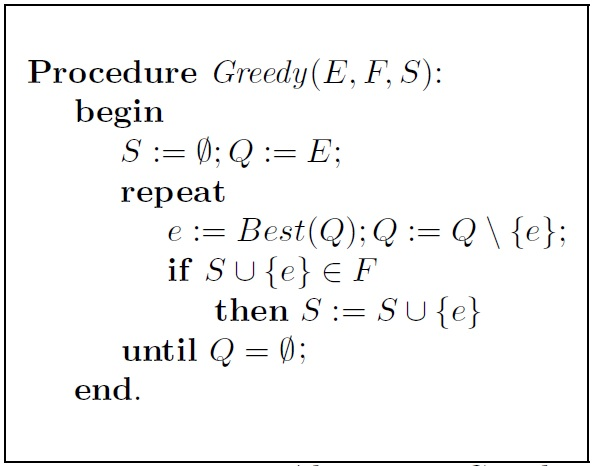
\includegraphics[scale=0.5]{ProceduraGreedy}  

Figura X: Algoritmo Greedy 
\end{center}


Nella procedura, \textbf{S} è l'insieme degli elementi di \textbf{E} che sono stati inseriti nella soluzione parziale corrente mentre \textbf{Q} è l'insieme degli elementi appartenenti ad \textbf{E} ancora da esaminare.
La procedura fa uso della sottoprocedura \textbf{Best} la quale fornisce il miglio elemento di \textbf{E} tra quelli ancora in \textbf{Q} sulla base di un prefissato criterio euristico. Nei successivi paragrafi presenteremo l' algoritmo greedy \textbf{nearest neighbour}, il quale rappresenta l' algoritmo costruttivo di riferimento per tutto il resto della tesi.

\vspace{2\baselineskip}
ALGORITMo NEAREST NEIGHBOUR
\vspace{2\baselineskip}

L' algoritmo nearest neighbour è stato uno dei primi algoritmi usati per determinare una soluzione del problema del commesso viaggiatore.
Partendo dal nodo etichettato 1, ad ogni iterazione esamina il nodo corrente \textit{i} e tutti gli archi che lo uniscono a nodi che non sono ancora visitati dal ciclo parziale: tra di essi seleziona l'arco [i, j], avente fra tutti la lunghezza minima, lo aggiunge alla soluzione parziale e definisce \textbf{j} come nuovo nodo corrente. L'algoritmo termina quando tutti i nodi sono stati visitati. 
Essendo un algoritmo greedy esso ricade nello schema generale precedentemente illustrato:\textbf{ E} è l'insieme degli archi del grafo, \textbf{Best} determina l'arco più promettente tra tutti quelli uscenti dal nodo corrente, il controllo "S $ \cup $ {e} $\in$ F " corrisponde a verificare che il nodo terminale \textbf{j} dell'arco [i, j] non sia già stato visitato.
Di seguito viene riportato un esempio di applicazione dell' algoritmo.

\begin{center}
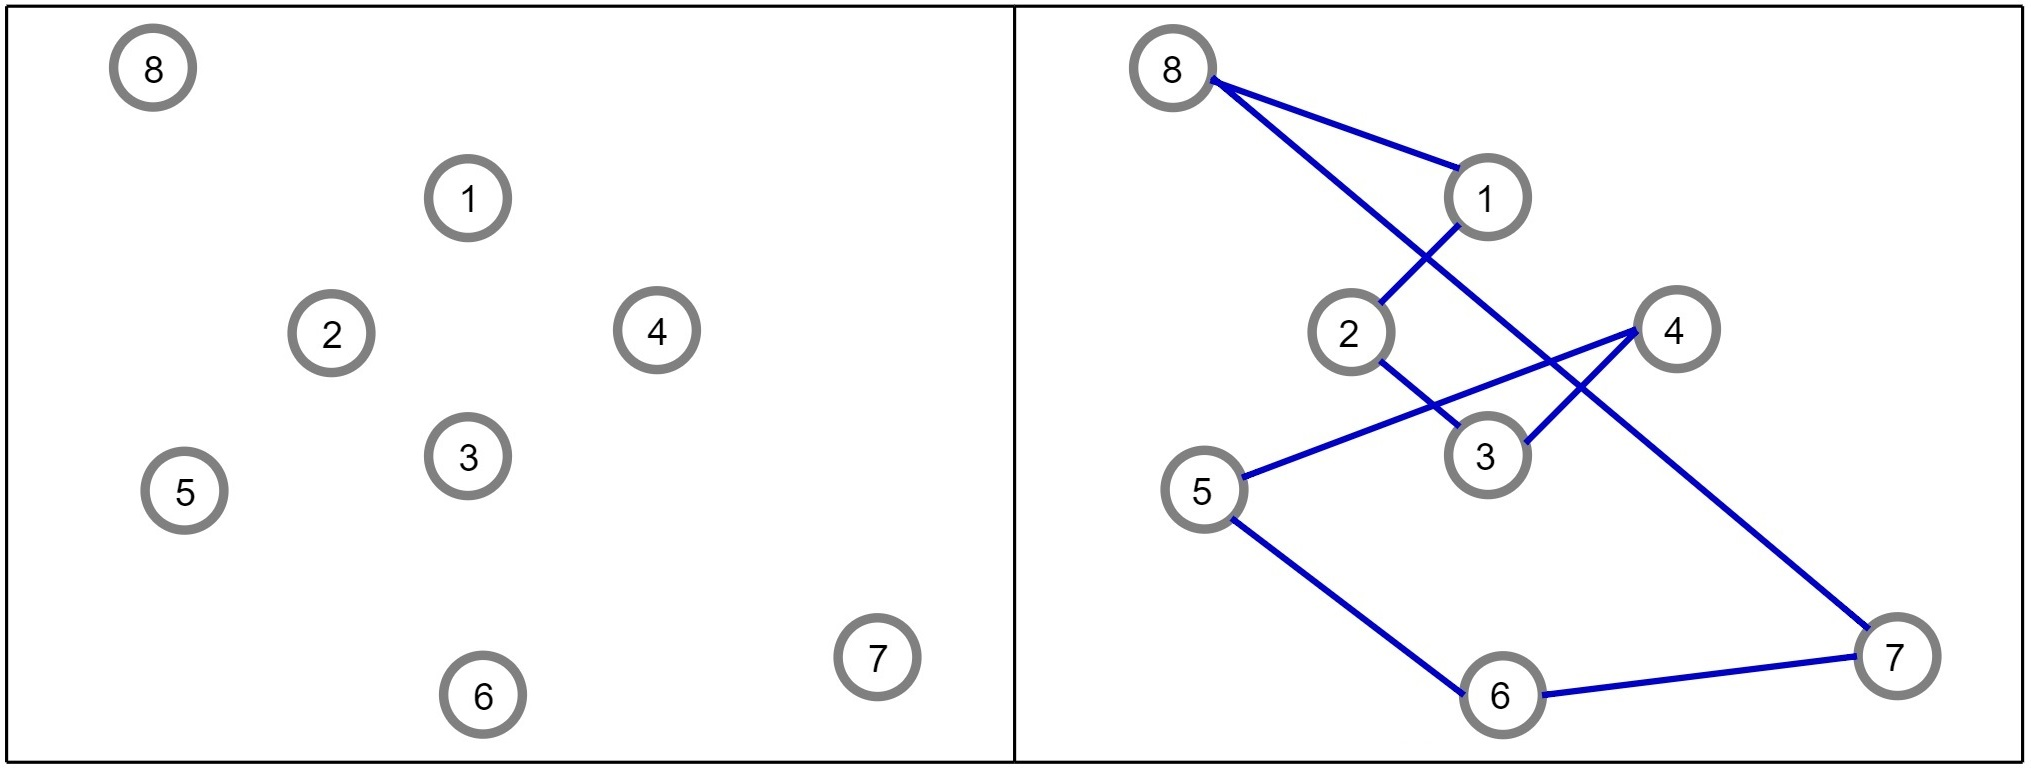
\includegraphics[scale=0.5]{ng}  

Figura X:Esempio di algoritmo Nearest Neightbor
\end{center}

L'algoritmo risulta di semplice implementazione e di complessità ridotta (O(n^2), migliorabile con particolari strutture dati) ma ha prestazioni scadenti in termini di soluzioni prodotte. 
Lo svantaggio di applicare questo algoritmo sta nell'impossibilità di prevedere gli sviluppi finali che esso comporta. Dai vantaggi immediati in termini di lunghezza comportano degli svantaggi ai passi successivi: le iterazioni successive producono archi molto dispendiosi che oltretutto si intersecano tra di loro. Quest' ultimo fatto è matematicamente dimostrabile essere sinonimo di non ottimalità. 

\textit{[Non ho messo qui l' implementazione dell' algoritmo perchè noi non abbiamo implementato il Nearest Neightbor come lo ho presentato qui perchè è stata randomizzata la scelta della Best.]}

\vspace{2\baselineskip}
ALGORITMI MIGLIORATIVI
\vspace{2\baselineskip}

Gli algoritmi migliorativi sono basati su un'idea estremamente semplice ed intuitiva: data una soluzione ammissibile \textbf{x}, relativa ad un problema di ottimizzazione, si esaminano le soluzioni ad essa "vicine" in cerca di una soluzione ammissibile migliore in termine di funzione obiettivo. 
Per poter definire il concetto di "vicinanza" è necessario definire prima il concetto di \textbf{mossa}. Una mossa è una operazione di modifica (caratteristica dell' algoritmo migliorativo) che viene eseguita su \textbf{x} e che ha come conseguenza la generazione di un insieme di soluzioni ammissibili le quali costituiscono l' intorno di \textbf{x}, che verrà indicato con \textbf{N(x)}. Le soluzioni che appartengono a N(x), in termini informali, sono dette "vicine" ad \textbf{x} poiché differiscono da \textbf{x} "solo per una mossa". 

Una volta definito N(x) questo viene esplorato secondo due possibili strategie che sono \textbf{first improvement} e \textbf{steepest descent}. Nel primo caso l'esplorazione dell' intorno termina non appena si trova una soluzione migliore di quella corrente. Nel secondo caso, invece, lo si esplora comunque tutto cercando il massimo miglioramento che quel vicinato consente di ottenere. 

Qualora esista una soluzione \textbf{y} migliore di \textbf{x}, il procedimento viene iterato esplorando N(y); viceversa  l'algoritmo si arresta. Se la soluzione determinata dall'algoritmo non coincide con la soluzione ottima del problema, questa risulta essere un \textbf{ottimo locale}. Poiché da un punto di vista matematico il processo di ricerca analizza, ad ogni interazione, un intorno della soluzione corrente, gli algoritmi migliorativi vengono anche chiamati\emph{ algoritmi di ricerca locale}.

Tranne alcuni casi particolari in cui la funzione obiettivo ha determinate caratteristiche di convessità, nella grande maggioranza dei problemi reali la funzione obiettivo da minimizzare presenta un grande numero di minimi locali, talora anche molto lontani dal minimo globale. In effetti, una delle fortunate eccezioni è il metodo del simplesso per la programmazione lineare. Il metodo del simplesso è infatti un algoritmo di ricerca locale, in cui si visitano le basi ammissibili di un sistema del tipo Ax = b, e l'intorno è composto da tutte le basi che differiscono per una sola variabile dalla  base corrente. La convessità della funzione obiettivo ci garantisce che il minimo locale trovato dal simplesso è anche globale.

\vspace{2\baselineskip}
ALGORITMO K-OPT
\vspace{2\baselineskip}

L' algoritmo migliorativo più consolidato per il TSP  prende il nome di \textbf{k-opt} la cui mossa, applicata ad un circuito hamiltoniano, consiste in uno scambio di \textbf{k} archi producendo \textbf{k} percorsi differenti che vengono ricollegati tra loro con l' introduzione di altri \textbf{k} archi. La mossa che produce la variazione minima coinvolge lo scambio di \emph{coppie} di archi in soluzione con archi non in soluzione: in questo caso l' algoritmo prende il nome di 2-opt. Data una soluzione ammissibile \textbf{x}, l'intorno N(x) contiene al suo interno tutti i cicli Hamiltoniani che si possono ottenere da \textbf{x} selezionando due archi  [i,j] e [h, k] non consecutivi\footnote{Se i due archi eliminati fossero adiacenti l'unico modo di riottenere una soluzione ammissibile riproporrebbe la soluzione di partenza.} del ciclo e sostituendoli con [i,h] e [j,k] o con [i,k] e [j,k]. Fra le due possibilità solamente una è lecita poiché consente di riottenere un ciclo hamiltoniano: supponendo (senza perdita di generalità) che i lati siano sostituiti con [i,h] e [j,k] , lo scambio produce una soluzione avente un costo minore(e quindi migliore) se: 

$$c_{ih} + c_{kj} < c_{ij} + c_{hk}$$


Poiche' gli archi in un ciclo hamiltoniano sono \textit{n}, la dimensione del vicinato di una soluzione (e dunque il tempo necessario a esplorarlo) è O(n^2). Tale complessità è ancora accettabile, e dunque un algoritmo di ricerca locale basato su questo vicinato risulta abbastanza efficiente. Chiaramente, all'aumentare di \textit{k} aumenta anche la grandezza del vicinato, e dunque il tempo di calcolo necessario a esplorarlo, che sarà ovviamente O(n^k).Tuttavia, se la grandezza di un vicinato aumenta, si può sperare che aumenti pure l'efficacia del singolo passo di ricerca locale. Trovare il miglior compromesso tra complessità dell'esplorazione del vicinato e qualità della soluzione è uno dei punti chiave di un approccio di ricerca locale.
Nel caso del TSP, alcuni esperimenti fatti da Lin alla fine degli anni '50 hanno mostrato che, passando da k =2 a k = 3 si ha un miglioramento sensibile della qualità della soluzione trovata, che giustifica pienamente l'aumento di carico computazionale. Miglioramenti praticamente trascurabili si hanno invece per $k > 3$.

\vspace{2\baselineskip}
METODO TwoOpt
\vspace{2\baselineskip}

Il metodo TwoOpt implementa l' algoritmo 2-Opt discusso nel paragrafo precedente e ha la seguente intestazione:

\begin{lstlisting}
public static void TwoOpt(Instance instance, PathStandard pathG)
\end{lstlisting}

Dove:

\begin{itemize}
    \item \textbf{instance}: rappresenta il valore del taglio;
    \item \textbf{pathG}: rappresenta il percorso sul quale l' algoritmo viene eseguito.
\end{itemize}

Sia \textbf{x} la soluzione corrente e N(x) il suo intorno, la ricerca di una soluzione migliore x* in N(x) avviene per enumerazione e termina una volta identificato uno scambio migliorativo, ossia si applica la politica first improvement. Poichè il vettore che codifica x ne induce una orientazione che viene perduta all' atto delle scambio dei lati, è stato necessario realizzare un metodo \textbf{SwapRoute}, appartenente alla classe Utility, il quale fornisce una orientazione a x*. Il metodo termina quando non è più possibile effettuare miglioramenti, in generale in un ottimo locale.

\begin{lstlisting}

int indexStart = 0;
int cnt = 0;
bool found = false;

do
{
   found = false;
   int a = indexStart;
   int b = pathG.path[a];
   int c = pathG.path[b];
   int d = pathG.path[c];

   for (int i = 0; i < instance.NNodes - 3; i++)
   {
      double distAC = Point.Distance(instance.Coord[a], instance.Coord[c], instance.EdgeType);
      double distBD = Point.Distance(instance.Coord[b], instance.Coord[d], instance.EdgeType);
      double distAD = Point.Distance(instance.Coord[a], instance.Coord[d], instance.EdgeType);
      double distBC = Point.Distance(instance.Coord[b], instance.Coord[c], instance.EdgeType);

      double distTotABCD = Point.Distance(instance.Coord[a], instance.Coord[b], instance.EdgeType) +
      Point.Distance(instance.Coord[c], instance.Coord[d], instance.EdgeType);

      if (distAC + distBD < distTotABCD)
      {
            Utility.SwapRoute(c, b, pathG);
            pathG.path[a] = c;
            pathG.path[b] = d;
            pathG.cost = pathG.cost - distTotABCD + distAC + distBD;
            indexStart = 0;
            cnt = 0;
            found = true;
            break;
      }
            c = d;
            d = pathG.path[c];
    }

    if (!found)
    {
        indexStart = b;
        cnt++;
    }

} while (cnt < instance.NNodes);
    

\end{lstlisting}


\vspace{2\baselineskip}
MULTISTART
\vspace{2\baselineskip}
 
Qualora l' algoritmo di ricerca locale converga rapidamente verso un ottimo locale, potrebbe rimanere tempo a disposizione per esplorare altre zone della regione ammissibile nella speranza di trovare soluzioni migliori. Poichè  l'ottimo locale determinato da un algoritmo di ricerca locale dipende dalla \textbf{soluzione ammissibile iniziale}, il modo più semplice per esplorare zone differenti della regione ammissibile è quello di generare un' insieme di soluzioni iniziali ed eseguire l'algoritmo di ricerca locale a partire da ciascuna di esse, quindi selezionare la migliore delle soluzioni così ottenute. 
Per quanto riguarda l' algoritmo nearest neightbor, un possibile modo per ottenere \textbf{n} soluzioni differenti, dove n è il numero dei nodi del grafo, è randomizzare il punto di partenza. Questa tecnica di randomizzazione non è particolarmente efficiente poichè se il grafo non ha molti nodi si hanno pochi circuiti a disposizione su cui eseguire gli algoritmi di ricerca locale. 
Un secondo modo per generare soluzioni differenti fra loro,valido per tutti gli algoritmi greedy, consiste nel rendere non deterministica la scelta della Best, in modo che, se l'algoritmo viene richiamato più volte, almeno in linea di principio, ad ogni esecuzione vengono fatte scelte differenti e generate soluzioni alternative. Algoritmi greedy in cui la funzione  Best è non deterministica prendono il nome di \textbf{GRASP} (Greedy Randomly Adaptive Search Procedure). Naturalmente rendere non deterministica la scelta della Best non significa rendere completamente casuale la scelta dell' elemento da aggiungere alla soluzione corrente; significa semplicemente che con una probabilità non nulla l' algoritmo può selezionare elementi che, anche se non sono la miglior scelta possibile, non si discostano di molto da essa. La combinazione di un algoritmo di ricerca locale e di un'euristica randomizzata viene denominato metodo \textbf{multistart}: il multistart da noi realizzato prevede di utilizzare l' algoritmo nearest neightbor, opportunamente randomizzato, per produrre circuiti hamiltoniani, ai quali viene applicato il metodo  2-opt. Prima di discutere il codice prodotto, nel successivo paragrafo si illustra come in linguaggio C# avviene la generazione dei numeri random utilizzati per randomizzare l' algoritmo  nearest neightbor. 

\vspace{2\baselineskip}
GENERAZIONE NUMERI CASUALI - SEMERANDOM
\vspace{2\baselineskip}

Per generare un numero casuale è sufficiente istanziare la classe Random ed invocare sull' istanza creata il metodo \textbf{Next} o \textbf{NextDouble}. Per esempio nel caso in cui si voglia generare un numero casuale intero tra 1 e 99 è necessario scrivere le seguenti righe di codice:

\begin{lstlisting}

Random random = new Random();
int nun = random.Next(1,100);

\end{lstlisting}

I numeri random sono generati, a partire da un valore d' inizializzazione chiamato \textbf{seme}, da un algoritmo matematico. Per sua natura l' algoritmo è deterministico: se si fornisce in input lo stesso seme genererà sempre la medesima sequenza di numeri. Per tale ragione il valore del seme viene derivato dall'orologio di sistema all' atto della  creazione dell' istanza della classe Random qualora si utilizza il costruttore di default. In questo modo, non essendo predicibile il valore del seme, la sequenza di numeri generati dall' algoritmo risulta essere sistematicamente casuale. 

L' orologio di sistema non sempre risulta un buon valore da utilizzare per settare il seme. Si supponga di avere la necessità di creare due oggetti diversi della classe Random: qualora quest' ultimi siano creati uno di seguito all' altro avranno entrambi il medesimo seme poichè l' orologio di sistema risulta lo stesso nel lasso di tempo che il processore impiega ad eseguire le due istruzioni.

Per constatare ciò si è realizzato il seguente programma:

\begin{lstlisting}

Random rdn1 = new Random();
Random rdn2 = new Random();

for (int i = 0; i < 10; i++)
{
    Console.WriteLine(rdn1.Next(1, 10) + "-" + rdn2.Next(1, 10));
}
Console.ReadLine();

\end{lstlisting}

Il cui output, come previsto, risulta mostrato in Fig C.

\begin{center}
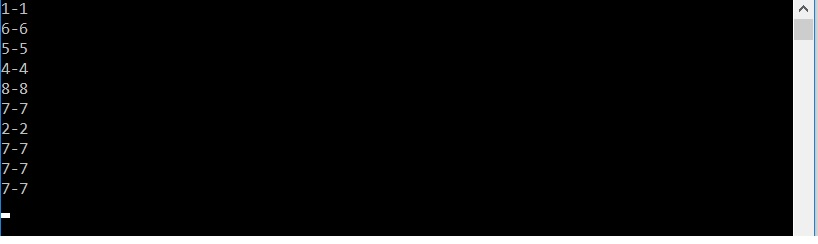
\includegraphics[scale=0.5]{output}  

Figura X: Output 

\end{center}

Per ovviare a questa problematica la classe Random dispone di un secondo costruttore che riceve come parametro un intero che setta il valore del seme: sarà a questo punto compito del programmatore passare valori casuali e  differenti all' atto della creazione delle due istanze della classe Random.

\vspace{2\baselineskip}
FUNZIONE NEAREST NEIGHTBOR
\vspace{2\baselineskip}

L' intestazione del metodo risulta essere:

\begin{lstlisting}

 public static PathGenetic NearestNeightbor(Instance instance, Random rnd, List<int>[] listArray)

\end{lstlisting}


Dove:

\begin{itemize}
    \item \textbf{instance}: oggetto della classe \textit{Instance} contenente tutti i dati che descrivono l'istanza del problema del Commesso Viaggiatore fornita in ingresso dall' utente;
    \item \textbf{rnd}: istanza della classe \textit{Random} precedentemente inizializzato con un seme random diverso per ogni iterazione del programma;
    \item \textbf{listArray}: lista in cui all'indice \textbf{i} è presente un vettore di dimensione instance.Nnodes al cui interno sono, in ordine crescente rispetto alla distanza assunta dal nodo \textbf{i}, presenti gli indici associati ai nodi del grafo.
\end{itemize}

Il circuito prodotto dal metodo viene memorizzato all'interno del vettore \textbf{heuristicSolution} in cui alla generica posizione \textbf{i} è collocato il nodo successivo al nodo \textbf{i}.Il vettore \textbf{availableIndexes} di tipo bool è un vettore di supporto che memorizza all'indice \textbf{i} il valore logico \textbf{true} se il nodo \textbf{i} è già stato visitato, \textbf{false} altrimenti. Il nodo di partenza sul quale l' algoritmo comincia la costruzione della soluzione si è scelto di renderlo casuale per i motivi forniti precedentemente. Per quanto riguarda la randomizzazione della scelta locale
\begin{lstlisting}

...

\end{lstlisting}

Una volta definito il nodo di partenza i restanti nodi son ottenuti attraverso un ciclo \textit{for}: alla generica iterazione \textbf{i} del ciclo, sfruttando la struttura dati \textbf{listArray} e la funzione \textbf{RndPlus} si memorizza all'interno della variabile \textbf{nextIndex} il nodo successivo visitato dal percorso sempre che questo sia stato ancora visitato. Per verificarne la disponibilità si utilizza l'array \textit{availableIndexes}, qualora non sia possibile utilizzare tale nodo si passa al successivo più vicino.


\begin{lstlisting}

....
\end{lstlisting}


\vspace{2\baselineskip}
METAEURISTICI
\vspace{2\baselineskip}

L' algoritmo multistart è una tecnica per sfuggire ai minimi locali ma, tipicamente, non risulta essere la tecnica più efficiente a tal scopo. 

In generale infatti, una ripartenza da un punto casuale "cancella la storia" dell'algoritmo: l'evoluzione successiva è completamente indipendente da tutto quello che è accaduto prima della ripartenza. In altri termini, il metodo multistart non è in grado di sfruttare in alcun modo l'informazione generata durante le ricerche locali precedenti per "guidare" la ricerca locale corrente. 

E' noto che per molti problemi le soluzioni di buona qualità sono normalmente abbastanza  "vicine" (in termini di numero di mosse) le une alle altre; quindi, l'aver determinato una "buona" soluzione fornisce una qualche forma di informazione che il metodo multistart non tiene in alcun modo in considerazione. Al contrario, la ricerca locale ha un qualche tipo di informazione sulla "storia" dell'algoritmo, data proprio dalla soluzione corrente. 
Quanto detto ha portato, a partire dagli anni '80, la ricerca di metodi sistematici per generalizzare la ricerca locale e sfuggire ai minimi locali ha prodotto numerosi risultati, chiamati \textbf{metaeuristici}. 
Il meccanismo di base utilizzato da questi algoritmi per muoversi nello spazio di ricerca è quello visto per la ricerca locale, cioè l'esplorazione di vicinati, nel quale però sono consentite\textbf{ mosse peggiorative}.
Quest'ultime risultano molto utili per spostarsi da un ottimo locale ad un ottimo locale ad esso vicino ma posso anche essere fonte di loop infiniti: ciò accade quando ripetutamente si ritorna in una soluzione precedentemente esplorata dopo un certo numero di mosse. 
Esistono diversi metaeuristici il letteratura, la nostra attenzione sarà focalizzata sul Variable neighborhood descent (VNS) e la Tabu Search; per ciascuno di essi sarà descritto il loro funzionamento,il meccanismo (caratteristico dell' algoritmo) implementato per evitare la creazione di loop e il codice realizzato per implementarli.

\vspace{2\baselineskip}
TABU
\vspace{2\baselineskip}

\vspace{2\baselineskip}
VNS
\vspace{2\baselineskip}

\vspace{2\baselineskip}
MATHEURISTICS
\vspace{2\baselineskip}

Gli algoritmi \textbf{matheuristics} nascono con l' obbiettivo di migliorare una soluzione di partenza ammissibile \textbf{x} sfruttando il modello matematico del MIP che si vuole risolvere. Analogamente a quanto visto per gli algoritmi di ricerca locale e metaeuristici, essi tentano di individuare una soluzione migliore x* all' interno di un intorno N(x) ottenuto, in questo ambito, modificando opportunamente il modello matematico del MIP di partenza. 

L' esplorazione di N(x) non avviene per enumerazione, come visto per gli algoritmi di ricerca locale, ma avviene tramite un solver che, in questo contesto, può essere visto come una “black-box” che risolve il subMIP corrente. Poiché al giorno d' oggi i solver risultano essere estremamente efficienti, gli algoritmi matheuristics consentono,tipicamente, di esplorare l' intorno N(x) in breve tempo. 
I matheuristici posso essere applicati a qualunque soluzione ammissibile x; ciò nonostante per apprezzarne davvero la potenza tipicamente vengono applicati successivamente all' esecuzione di un algoritmo migliorativo o, meglio ancora, al termine del multistart o di un metaeuristico. Questo perchè, molto spesso, le tecniche mostrate precedentemente tendono tutte a saturare in prossimità di una soluzione molto buona \textbf{\overline{x}}, ma che non rappresenta l' ottimo. Fornendo tale soluzione ad un matheuristics esso è in grado di migliorarla in brevissimo tempo e, dipendentemente dal costo di \textbf{\overline{x}} e del time limit residuo, persino di raggiungere l' ottimo globale. Si osserva che esiste una notevole differenza fra l' ottenere l' ottimo da un algoritmo esatto e calcolare l' ottimo seguendo il procedimento precedentemente discusso: mentre nel primo caso l' ottimo è certificato, nel secondo caso non si ha modo di sapere, a meno che non si conosca a priori il suo costo, se la soluzione restituita all' utente terminato il time-limit rappresenta l' ottimo oppure no.

Il punto saliente di questi metodi consta nella determinazione del vicinato di una soluzione di partenza \textbf{x}. Tale scelta è tutt'altro che banale, ed è la chiave per ottenere un metodo efficiente. Uno schema comunemente usato è di scegliere un certo numero di variabili della soluzione di riferimento \textbf{x} e fissarle, lasciando libere altre. Questo modo di procedere è detto\textbf{ hard variable fixing}; il suo principale svantaggio è rappresentato nel difficile problema della scelta di quali variabili sia opportuno fissare e quali lasciare libere. In contrapposizione a questa tecnica è possibile pensare ad un differente modo di procedere, il cosiddetto \textbf{soft variable fixing}, che consiste invece nel far sì che un certo numero di variabili restino immutate, ma senza conoscere a priori quali siano, lasciando che sia il solver ad effettuare la scelta ottimale fra tutte quelle possibili.


\vspace{2\baselineskip}
HARD FIXING
\vspace{2\baselineskip} 

L' hard fixing è una tecnica euristica che, data una soluzione ammissibile \textbf{x_H}, consiste nel fissare in soluzione lati che fanno parte di \textbf{x_H}. La soluzione \textbf{x_H} può essere ottenuta utilizzando un qualunque algoritmo costruttivo oppure Cplex fornendogli un time limit che ragionevolmente possa essere considerato breve per l' istanza che si vuole risolvere. Esistono varie politiche di fissaggio dei lati. Una strategia possibile consiste nello scansionare tutti i lati che costituiscono x_H e fissare in soluzione le variabili ad essi associati con probabilità \textbf{p}. Una seconda strategia consiste invece nel fissare in soluzione gli $m$ lati più corti di x_H; tale politica prende origine dall' idea intuitiva per cui lati lunghi poco probabilmente faranno parte della soluzione ottima. 
Il fissaggio di alcune variabili induce la definizione di un intorno N(x_H) al cui interno sono presenti tutti i tour aventi tali variabili fissate: l' esplorazione dell' intorno non avviene più tramite enumerazione come visto per gli algoritmi migliorativi, ma avviene utilizzando Cplex.//
Naturalmente maggiore è il numero di variabili fissate (ossia più elevati sono p o m a seconda della strategia di fissaggio usata), minore saranno le operazioni di branching e quindi conseguentemente i nodi dell' albero decisionale. Un minor numero di nodi implica un minor numero numero di rilassamenti continui da risolvere e ciò non può che velocizzare Cplex nel calcolo della soluzione ottima del subMIP.
 
Tuttavia la soluzione prodotta non sarà in generale un ottimo globale poichè con un \textit{p} o un \textit{m} molto elevato risulta poco probabile fissare in soluzione tutte le variabili che appartengono alla soluzione ottima. 
Qualora il time limit residuo non risulta nullo, è quindi opportuno nelle iterazioni successive diminuire il valore di tali parametri. Tipicamente si preferisce la prima strategia poichè consente dopo un certo numero k di iterazioni, dove k può essere molto elevato, di calcolare la soluzione ottima essendo che si fissano ad ogni iterazioni variabili in maniera random e ,poichè gradualmente p viene diminuito, è facile in una iterazione vengano fissata tutte variabili che appartengono alla soluzione ottima. La seconda strategia da questo punto di vista risulta più scadente visto che, anche se solo un lato fra quelli più corti non appartiene alla soluzione ottima, esso viene comunque fissato impedendo a Cplex di calcolare l' ottimo.

\vspace{2\baselineskip} 
WARM-START
\vspace{2\baselineskip} 

Qualora si disponga di una soluzione del problema in esame, per esempio ottenuta da un run precedente di un solver o da un algoritmo euristico, è possibile fornirla a Cplex il quale, prima di iniziare il B&C, la processa durante la fase di ottimizzazione. Tale soluzione prende il nome di  \textbf{warm-start} o \textbf{MIP start} e qualora risulti una soluzione ammissibile, viene installata come incumbent. 
Poter disporre di un incumbent è molto importante poichè consente a Cplex di dichiarare sondati nodi il cui costo della soluzione del rilassamento continuo risulta essere superiore rispetto al costo dell' incumbent(criterio di bounding). Avere un incumbent consente inoltre a Cplex di utilizzare euristici che necessitano di esso, come ad esempio gli euristici \textbf{RINS} e \textbf{polishing} che saranno discussi nel paragrafo X. Per poter installare un MIPStart è necessario invocare sull' oggetto della classe Cplex in cui si definisce il modello il metodo \textbf{AddMIPStart} la cui firma è:

\begin{lstlisting}

public virtual int AddMIPStart(INumVar[] vars,double[] values)

\end{lstlisting}

Dove:

\begin{itemize}
    \item \textbf{vars}: Vettore contenente nella posizione i la i-esima variabile del modello
    \item \textbf{values}: Vettore contenente nella posizione i il valore della i-esima variabile del modello
\end{itemize}

La soluzione di partenza \textbf{x} è stata fornita a Cplex come MIP start. Si osserva che non è invece necessario fornire a Cplex un warm start nel caso in cui l' incumbent x_I venga aggiornato poichè, nonostante Cplex fissi ad "infinito" il valore dell' incument ogni qual volta inizia a risolvere il subMIP corrente, esso verifica se quest' ultimo risulta essere una soluzione ammissibile per il nuovo subMIP e in tal caso lo installa come incumbent. Per costruzione x_I risulta essere una soluzione ammissibile anche del subMIP corrente poichè questo è ottenuto fissano in soluzione variabili che appartengono proprio a x_I. Analogamente nel caso non venga aggiornato, in questo caso l'incument con cambia e all' iterazione successiva continua ad essere una soluzione ammissibile del subMIP corrente

\vspace{2\baselineskip}
PRE-PROCESSING
\vspace{2\baselineskip} 

Per ridurre il tempo necessario a Cplex per calcolare la prima soluzione migliore di x_I nell' intorno N(x_I), risulta estremamente utile eseguire una seconda fase di fissaggio di variabili. Mentre nella prima fase si fissano in maniera casuale le variabili appartenenti a x_I, in questa seconda fase, a partire dalle variabili fissate, se ne fissano altre a 0 in modo da ridurre la probabilità che la soluzione candidata da Cplex come incumbent abbia al suo interno dei subtour. La fase di pre-processing è quindi specifica per il problema del Commesso Viaggiatore, si consideri la figura X in cui in blu sono stati indicati i lati fissati in soluzione:

\begin{center}
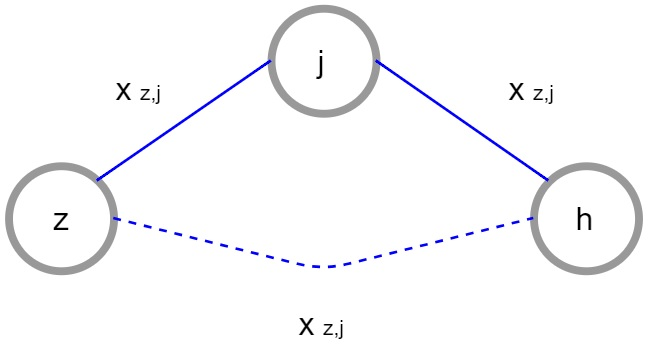
\includegraphics[scale=0.5]{PreProcessing}  

Figura X: Output 

\end{center}

Le variabili x_{1,3},x_{4,5} e x_{6,9}, per come si sono fissati i lati, dovranno necessariamente assumere il valore 0,altrimenti si avrebbe la presenza di uno o più subtour. 

Il metodo che realizza ciò è stato chiamato \textbf{PreProcessingTSP} ed ha la seguente firma:

\begin{lstlisting}

 public static void PreProcessing(Instance instance, INumVar[] x)

\end{lstlisting}

Dove:

\begin{itemize}
    \item \textbf{instance}: riferimento all' oggetto contenente tutte le informazioni relative all' istanza del Problema del Commesso Viaggiatore corrente;
    \item \textbf{x}: vettore contente le variabili del modello matematico;
\end{itemize}

L' algoritmo individua per ogni nodo, in cui incide almeno un lato fissato, la relativa componente connessa e memorizza per ognuno di essi il numero di lati ad esso incidenti. 

\begin{lstlisting} 
 
//Array that stored,for eache node, how many edges incise to it 
int[] cntNode = new int[instance.NNodes];
            
//Vector contenent for each node relative connected component
int[] compConn = new int[instance.NNodes];

//Array of List where are stored,for each connected component the nodes in which incise only a edge
List<int>[] externalNodes = new List<int>[instance.NNodes];

//Inizialization compConn
Utility.InitCC(compConn);

//Inizialization externalNodes
for (int i = 0; i < instance.NNodes; i++)
      externalNodes[i] = new List<int>();

for (int i = 0; i < instance.NNodes; i++)
{
    for (int j = i + 1; j < instance.NNodes; j++)
    {
          //Retriving the correct index position for the current link 
          int position = Utility.xPos(i, j, instance.NNodes);

           //if the edge is fixed 
            if (x[position].LB == 1)
            {
                 //Upgrade the array cntNode
                  cntNode[i] += 1;
                  cntNode[j] += 1;

                   //Set the connected component 
                   for (int k = 0; k < instance.NNodes; k++)
                   {
                        if ((k != j) && (compConn[k] == compConn[j]))
                           compConn[k] = compConn[i];                          
                    }

                   //Finally also the value relative to the node i are updated
                   compConn[j] = compConn[i];                                                                        
              }
       }
}
\end{lstlisting}
  
Per individuare i nodi i,j della variabile x_[i,j] da porre a 0 è sufficiente, per ogni nodo avente un solo lato indicente, inserirlo nella posizione i di un vettore di liste, dove i è compConn[i], cioè la componente connessa di quel nodo.
  
\begin{lstlisting}    
//For each connected component we determine the node which have only a edge incident 
for(int i = 0; i< instance.NNodes; i++)
{
     if (cntNode[i] == 1)
        externalNodes[compConn[i]].Add(i);
}
\end{lstlisting}

Infine si scandiscono tutte le liste appartenenti nel vettore externalNodes, qualora la lista k-esima contenente 2 nodi, questi per costruzione sono i nodi incidenti del lato da porre a 0 della componente connessa k-esima.//
Si osserva che, qualora la componente connessa sia formata da un solo lato, non dobbiamo ovviamente fissarlo a 0. 

\begin{lstlisting}  
//Fix to 0 the variable associated to the edge that create a subtour if is fix to 1 by Cplex
for (int i = 0; i < instance.NNodes; i++)
{
	if (externalNodes[i].Count == 2)
	{
		//Retriving the correct index position for the current link 
         int pos = xPos(externalNodes[i][0], externalNodes[i][1], instance.NNodes);

         //If the variabile is not previus fix, set the relative LB to 0
         if ((x[pos].UB == 1) && (x[pos].LB == 0))
            x[pos].UB = 0;
	}
}

\end{lstlisting}


\vspace{2\baselineskip}
IMPLEMENTAZIONE HARD FIXING
\vspace{2\baselineskip} 

Passiamo ora a discutere il metodo HardFixing realizzato, fornendo una panoramica del suo funzionamento e definendo quali scelte sono state adottate. La sua firma risulta essere:

\begin{lstlisting}

static void HardFixing(Cplex cplex, Instance instance, Process process, Random rnd, Stopwatch clock)

\end{lstlisting}

Dove:

\begin{itemize}
    \item \textbf{cplex}: riferimento oggetto contenente il modello da risolvere;
    \item \textbf{instance}: riferimento all' oggetto contenente tutte le informazioni relative all' istanza del Problema del Commesso Viaggiatore corrente;
    \item \textbf{process}: 
    \item \textbf{rdn}: istanza della classe Random utilizzata per la generazione dei numeri casuali;
    \item \textbf{clock}: 
\end{itemize}


La soluzione di partenza c_P è stata ottenuto applicando il metodo NearestNeightbor precedentemente discusso. Come accennato, i matheuristici risultano tipicamente applicati a soluzioni  con costi già particolarmente buoni, per tale ragione si è invocato il metodo TwoOpt su c_P il quale produrrà una soluzione x il cui costo risulta,tipicamente, inferiore rispetto a c_P. La soluzione così ottenuta è stata memorizzata nel formato utilizzato da Cplex e passata come MIPstart.

Visto che non si sono aggiunti i vincoli di subtour, per garantire che l' eventuale soluzione migliorativa che Cplex  individua nell' intorno corrente, non abbia cicli al suo interno è stato necessario installare la lazy callback.

\begin{lstlisting}

StreamWriter file;

//Vector used to encode the path that rappresent the best integer solution note
double[] currentIncumbentSol = new double[(instance.NNodes - 1) * instance.NNodes / 2];
            
//Cost of the best integer solution note
double currentIncumbentCost = Double.MaxValue;

List<int>[] listArray = Utility.BuildSLComplete(instance);

//Variable use to don't fix any candidate incumbent solution when lazy callback is invoke
bool BlockPrint = false;

const int VALUECONSITENOTIMPROV = 3;

//Defined the max number of consecutive run of cplex whithout finds a improvement of the incumbent
int consecutiveiterationNotImprov = VALUECONSITENOTIMPROV;

//Defined the percentage of edge in the current solution that fixed 
double percentageFixing = 0.8;

instance.BestSol = new double[(instance.NNodes - 1) * instance.NNodes / 2];

//Create the model
INumVar[] x = Utility.BuildModel(cplex, instance, -1);

//Create a heuristic solution
PathStandard heuristicSol = Utility.NearestNeightbor(instance, rnd, listArray);
            
//Apply 2-opt algorithm in order to improve the costo o the heiristicSol
TwoOpt(instance, heuristicSol);

//The heuristic solution is the Incumbent, translate the encode in the format used by Cplex
for (int i = 0; i < instance.NNodes; i++)
{
      int position = Utility.xPos(i, heuristicSol.path[i], instance.NNodes);
      //Set to one only the edge that belong to heuristic solution
      currentIncumbentSol[position] = 1;
}

currentIncumbentCost = heuristicSol.cost;

//Installation of the Lazy Constraint CallBack
            
TSPLazyConsCallback tspLazy = new TSPLazyConsCallback(cplex, x, instance, process, BlockPrint);
cplex.Use(tspLazy);
           
//Provide to Cplex a warm start
cplex.AddMIPStart(x, currentIncumbentSol);

//Set the number of thread equal to the number of logical core present in the processor
cplex.SetParam(Cplex.Param.Threads, cplex.GetNumCores());
\end{lstlisting}


Fra le politiche possibili per esplorare N(x), si è scelto nuovamente di utilizzare \textbf{first improvement}. Per applicare correttamente tale politica si è fissato il paramento \textbf{IntSolLim} interno a cplex al valore 2.

\begin{lstlisting}

cplex.SetParam(Cplex.LongParam.IntSolLim, 2);

\end{lstlisting}

Esso determina il numero di soluzioni che Cplex deve individuare prima di arrestarsi: è necessario settarlo a 2 poichè gli passiamo un warm-start sempre ammissibile per il modello corrente e ad ogni iterazione cplex riparte dall' incumbent di quella precedente per cui sempre Cplex ha una soluzione ammissibile.


La generica iterazione \textit{t} dell' algoritmo si sviluppa come segue: sia \textbf{x_I} la miglior soluzione calcolata da Cplex fino all' itarazine \textit{t}, ogni lato di \textit{x_I} viene fissato in soluzione con probabilità \textit{p} dal metodo \textbf{ModifyModel}. Fissare in soluzione la variabile \textit{x_i} equivale ad aggiungere al modello il vincoli $x_i = 1$ e togliere il vincolo di interezza 0<= x_i <= 1: il nuovo modello così ottenuto viene risolto da Cplex.

Alla prima soluzione ammissibile x* calcolata,il cui costo risulta inferiore rispetto ad \textit{x_I}, il solver viene arrestato e si pone x_I = x*. All' iterazione $t + 1$ vengono nuovamente fissate con probabilità $p$ variabili in soluzione appartenenti a \textit{x*}  iterando il procedimento discusso. Qualora invece in N(x_I) non esista una soluzione migliore di x_I, si modifica l' intorno di esplorazione, ovvero vengono fissate nuovamente in soluzione lati che appartengono x_I ma, poichè il processo di fissaggio è casuale, verranno fissate variabili differenti ottenendo così un intorno differente rispetto al precedente. Quando decidere di far diminuire p è tutt' altro che banale ed esistono svariate possibilità.//

[...]

//

Infine si è ripristinato il valore del lower bound di tutte le variabili per l' iterazione successiva.

\begin{lstlisting}

do
{
      //Modify the Model according to the current Incumbent solution
       Utility.ModifyModel(instance, x, rnd, percentageFixing, currentIncumbentSol);
              
       //Solve the model
       cplex.Solve();

        if (currentIncumbentCost > cplex.GetObjValue(Cplex.IncumbentId))
        {
             file = new StreamWriter(instance.InputFile + ".dat", false);

              currentIncumbentCost = cplex.GetObjValue(Cplex.IncumbentId);
              currentIncumbentSol = cplex.GetValues(x, Cplex.IncumbentId);

              //Print solution               
              for (int i = 0; i < instance.NNodes; i++)
              {
                  for (int j = i + 1; j < instance.NNodes; j++)
                  {
                      int position = Utility.xPos(i, j, instance.NNodes);

                       if (currentIncumbentSol[position] >= 0.5)
                       {
                              file.WriteLine(instance.Coord[i].X + " " + instance.Coord[i].Y + " " + (i + 1));
                              file.WriteLine(instance.Coord[j].X + " " + instance.Coord[j].Y + " " + (j + 1) + "\n");
                       }
                  }
              }

              file.Close();

              Utility.PrintGNUPlot(process, instance.InputFile, 1, currentIncumbentCost, -1);
              
              //Restorarion the variable consecutiveIterationNotImprov to the value VALUECONSITENOTIMPROV
              consecutiveiterationNotImprov = VALUECONSITENOTIMPROV;
        }
        else
        {
              /If don't have improvement decrease variable consecutiveIterationNotImprov
              consecutiveiterationNotImprov--;
        }
                                   
        if (consecutiveiterationNotImprov == 0)
        {
              if (percentageFixing > 0.2)
              {
                   percentageFixing -= 0.1;
                   consecutiveiterationNotImprov = VALUECONSITENOTIMPROV;
              }
              else
                  consecutiveiterationNotImprov = VALUECONSITENOTIMPROV;
         }

        //Restoration the lower and upper bound of all variable. 
        for (int i = 0; i < x.Length; i++)
        {
             x[i].LB = 0;
             x[i].UB = 1;
        }

} while (clock.ElapsedMilliseconds / 1000.0 < instance.TimeLimit);

instance.XBest = currentIncumbentCost;
instance.BestSol = currentIncumbentSol;

cplex.Output().WriteLine();


//Empty line
cplex.Output().WriteLine();

cplex.Output().WriteLine("x = " + instance.XBest + "\n");

if (Program.VERBOSE >= -1)
     cplex.ExportModel(instance.InputFile + ".lp");


\end{lstlisting}



\vspace{2\baselineskip}
METODO MODIFYMODEL (APPENDICE)
\vspace{2\baselineskip} 

Il metodo ModifyModel fissa in soluzione, con una certa percentuale p, lati che appartengono ad una soluzione ammissibile. La sua firma risulta essere:

\begin{lstlisting} 
public static void ModifyModel(Instance instance, INumVar[] x, Random rnd, double percentageFixing, double[] solution)
\end{lstlisting}

Dove:

\begin{itemize}
    \item \textbf{instance}: riferimento all' oggetto contenente tutte le informazioni relative all' istanza del Problema del Commesso Viaggiatore corrente;
    \item \textbf{x}: vettore contenente le variabili del modello;
    \item \textbf{rnd}: istanza della classe Random utilizzata per la generazione dei numeri casuali;
    \item \textbf{percentageFixing}: Probabilità con cui un lato viene fissato in soluzione;
    \item \textbf{solution}: Vettore che codifica la soluzione ammissibile su cui si fissano in soluzione i lati.
\end{itemize}


L' idea dell' algoritmo consiste nel scandire tutti i lati appartenenti alla soluzione ammissibile fornitagli in ingresso, invocare per ognuno lato il metodo \textbf{RandomSelect} e se ritorna 1 viene fissato il lato altrimenti no. Per fissarlo si pone semplicemente il LB della variabile ad esso associata a 1.  Il ciclo do - while serve per ripete il fissaggio qualora si fissino tutti i lati o non si vincoli solo un lato poichè non avrebbe senso a questo punto far partire cplex. Al termine del metodo viene effettuato il preprocessing discusso del paragrafo precedente.

\begin{lstlisting}

//Stored the number of variable fixed
int nVariabileFix = 0;

do
{
   nVariabileFix = 0;

   //Scan all edge that belong to the current heuristic solution
    for (int i = 0; i < x.Length; i++)
    {
        if ((solution[i] == 1))
        {
            //Whit a percentageFixing probability fix a edge belong to the current solution
             if (RandomSelect(rnd, percentageFixing) == 1)
             {
                   x[i].LB = 1;
                   nVariabileFix++;
             }
         }
     }

} while (nVariabileFix >= instance.NNodes - 1);
             
Utility.PreProcessingTSP(instance, x);

\end{lstlisting}


\vspace{2\baselineskip}
RINS
\vspace{2\baselineskip}

Nell’esplorazione di un albero di ricerca, generalmente due soluzioni sono a disposizione: la soluzione incumbent che è ammissibile rispetto al vincolo di interezza, ma non è ottima finché l’ottimizzazione non ha termine e la soluzione è caratterizzata da un valore migliore di quello della soluzione incumbentdel rilassamento continuo del nodo corrente che molto spesso non è intera, ma che è caratterizzata da un valore migliore di quello della soluzione incumbent.

L' algoritmo \textbf{RINS}(Relaxation Induced Neighborhood Search) è un algoritmo euristico che utilizza la tecnica dell' hard fixing ed è implementato all' interno di Cplex. 
Quali variabili fissare risulta essere un scelta molto importante poichè determina l' intorno che verrà da cplex esplorato. L' algoritmo RINS necessità di due soluzioni ammissibili come input e fissa in soluzione le variabili comuni sia ad x1 che a x2. 


\vspace{2\baselineskip}
POLISHING
\vspace{2\baselineskip}

L' algortitomo polishing è un euristico che sfrutta l' algoritmo RINS all' interno dell' algoritmo genetico. 

\vspace{2\baselineskip}
LOCAL BRANCHING
\vspace{2\baselineskip}


\vspace{2\baselineskip}
IMPLEMENTAZIONE LOCAL BRANCHING
\vspace{2\baselineskip}

\vspace{2\baselineskip}
LOCAL BRANCH SIMMETRICO
\vspace{2\baselineskip} 


\vspace{2\baselineskip}
ALGORITMI GENETICI
\vspace{2\baselineskip}

Gli Algoritmi Genetici (\textit{AG}), proposti nel 1975 da J.H. Holland, sono un modello computazionale idealizzato dall'evoluzione naturale darwinista. L'aggettivo "genetico" deriva dal fatto che il modello evolutivo darwiniano trova spiegazioni nella branca della biologia detta genetica e dal fatto che tali algoritmi attuano meccaniche concettualmente simili a quelli dei processi biochimici scoperti da questa scienza. I principi fondamentali che consentono la nascita e lo sviluppo di un processo evolutivo che porta all'evoluzione di una specie sono la \textbf{selezione naturale} e la \textbf{varietà del genotipo}\footnote{Il termine \textit{genotipo} indica la costituzione genetica di un organismo o di un gruppo di individui} della popolazione.
La selezione naturale è il meccanismo grazie al quale si ha un progressivo e cumulativo aumento della frequenza degli individui aventi caratteristiche ottimali per l'ambiente in cui essi vivono poiché solo quelli che meglio si adattano ad un certo habitat riescono a sopravvivere e a riprodursi.
I meccanismi generatori della variazione del genotipo della popolazione sono sostanzialmente due:

\begin{itemize}
    \item Un processo di \textbf{riproduzione} nel quale gli individui, detti genitori, si accoppiano producendo di nuovi, detti figli, il cui patrimonio genetico risulta pertanto una combinazione di quello dei genitori;
    \item Un processo di \textbf{mutazione} che colpisce i figli i quali subiscono una modifica del patrimonio genetico ereditato dai genitori per effetto dell'ambiente che li circonda;
\end{itemize}

I cambiamenti che si verificano da una generazione all'altra risultano essere molto piccoli ma, dato che sopravvivono soprattutto quelli positivi, un loro accumulo porta nel tempo a grandi cambiamenti.
La ricerca parte da una popolazione iniziale di individui, detti cromosomi, che rappresentano ipotetiche soluzioni al problema dato. Ogni individuo della popolazione viene codificato da un vettore\footnote{Oltre alla codifica vettoriale in letteratura è possibile trovare anche quella ad albero. Tuttavia essa viene utilizzata per codificare gli individui della popolazione nell'ambito della programmazione genetica (che è?????????).} i cui elementi contengono simboli appartenenti ad un alfabeto finito, detti geni. Ad ogni soluzione è associato un valore determinato da una funzione chiamata \textbf{Fitness} il cui scopo è di determinare la bontà di un individuo nel risolvere il problema in questione.
Così come nella natura solamente gli individui che meglio si adattano all' ambiente sono in grado di sopravvivere e riprodursi, anche negli algoritmi genetici le soluzioni migliori sono quelle che hanno la maggiore probabilità di trasmettere i propri geni alle generazioni future.
Come vedremo in seguito sono fondamentalmente tre le caratteristiche determinanti per un algoritmo genetico: determinare quale funzione di fitness si andrà ad utilizzare, partendo dalla attuale generazione decidere come creare un pull di possibili candidati per quella successiva ed infine come selezionare tra questi ultimi quelli che sopravviveranno.
Essendo la definizione delle funzione di fitness direttamente dipendente da quale tipo di problema si desidera studiare, concludiamo questa introduzione elencando solamente quali operatori genetici è possibile applicare per definire le restanti due caratteristiche di un algoritmo.


\vspace{2\baselineskip}
OPERATORI GENETICI
\vspace{2\baselineskip}

In questo paragrafo vengono trattati i principali operatori genetici applicabili ai cromosomi. Per ogni operatore vengono inoltre descritte le principali varianti che si possono trovare in letteratura.


\vspace{2\baselineskip}
OPERATORE DI CROSSOVER
\vspace{2\baselineskip}

Il crossover è una metafora della riproduzione in cui il materiale genetico dei discendenti è una combinazione di quello dei genitori. Di seguito sono indicati alcuni dei metodi più comuni per creare un \textit{figlio} partendo da due \textit{genitori}, le instanze così ottenute vanno a far parte di quelle candidate alla sopravvivenza per la generazione successiva:

\begin{itemize}
    \item \textbf{Crossover ad un punto}: date due soluzioni si tagliano i loro vettori di codifica in un punto casuale o predefinito per ottenere due teste \{$H_a, H_b$\} e due code\{$T_a, T_b$\}, si possono costruire quindi altrettante soluzioni distinte combinando la testa di un genitore con la coda dell'altro $S_1 = H_a \cup T_b , S_2 = H_b \cup T_1$;
    
    \item \textbf{Crossover a due punti}: date due soluzioni si tagliano i loro vettori di codifica in due punti predefiniti o casuali al fine di ottenere una coppia di teste\{$H_a, H_b$\}, parti centrale \{$I_a, I_b$\} ed code \{$T_a, T_b$\}. Le due soluzioni sono ottenute scambiando le due parti centrali nei genitori $S_1 = H_a \cup I_b \cup T_a , S_2 = H_b \cup I_a \cup T_b$;
    
    \item \textbf{Crossover uniforme}: consiste nello scambiare casualmente elementi tra le soluzioni candidate all'evoluzione;
    
    \item \textbf{Crossover aritmetico}: consiste nell'utilizzare un'operazione aritmetica per creare la nuova soluzione, ad esempio eseguendo una \textit{XOR} o una \textit{AND} tra elementi dei genitori se interpretati come una sequenza binaria;
\end{itemize}

\begin{center}
    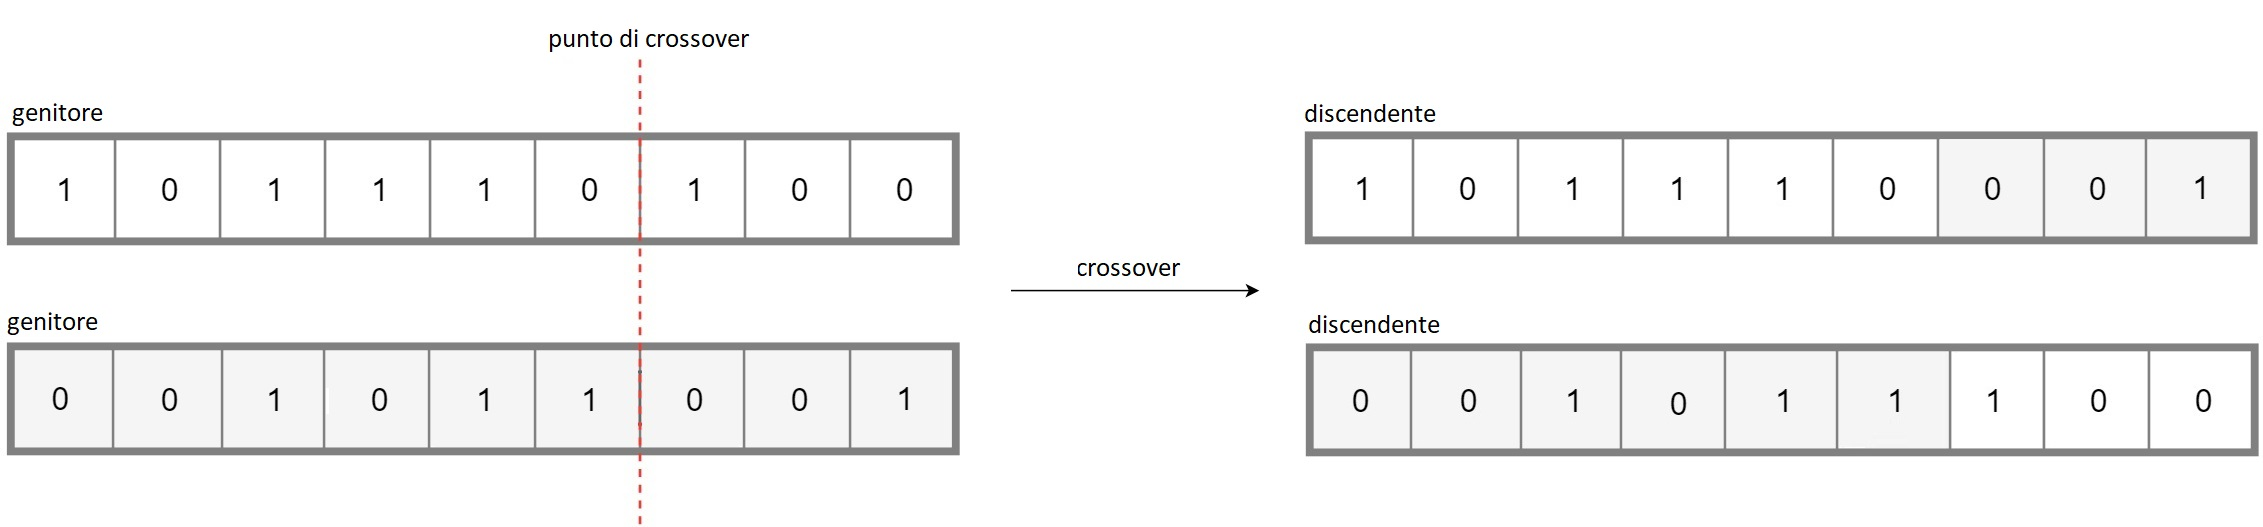
\includegraphics[scale=0.5]{selezioneSP}
    
    Figura 3: Esempio di operatore di crossover
\end{center}


\vspace{2\baselineskip}
OPERATORI DI SELEZIONE
\vspace{2\baselineskip}

A causa di complessi fenomeni di interazione non lineare, non è sempre vero che da due soluzioni promettenti ne nasca una terza \textit{migliore} né che da due soluzioni con valori di fitness basso venga generato un figlio \textit{peggiore}. Pertanto non è statisticamente conveniente utilizzare i soli elementi con valori di fitness elevata sia durante la scelta dei genitori che durante la scelta di quali elementi faranno parte della generazione successiva. Per quanto riguarda quest'ultimo caso, oltre al semplice valore di fitness, vengono prese in considerazione particolari tecniche di \textit{selezione}. Le più comuni sono:

\begin{itemize}
    \item \textbf{Selezione a roulette}: la probabilità che una soluzione venga scelta per far parte della successiva generazione è direttamente proporzionale al valore restituito dalla funzione di fitness. Immaginiamo quindi di avere a disposizione una roulette la cui ruota viene divisa in sezioni tutte assegnate ai vari candidati, la loro grandezza è quindi proporzionale all'idoneità dell'individuo. La selezione è banalamente ottenuta con molteplici rotazioni della roulette tenendo conto che un individuo non può essere selezionato più volte. Questa tecnica presenta dei problemi nel caso in cui le sezioni della ruota risultino tra loro eccessivamente sbilanciate in ampiezza, le soluzioni peggiori vengono selezionate troppo raramente e questo per quanto già esposto non è necessariamente un bene;

    \item \textbf{Selezione di Boltzmann}: le soluzioni vengono scelte con un grado di probabilità che, agli inizi dell'algoritmo, favorisce \textit{l'esplorazione} mentre più avanti tende a stabilizzarsi. Questa tecnica ritiene utile, in un primo momento, consentire agli individui meno idonei di riprodursi quasi quanto quelli migliori, e far procedere lentamente la selezione così da mantenere una certa diversità all'interno della popolazione. In seguito si rafforza la selezione per favorire maggiormente gli individui ad alta idoneità, presumendo che la fase iniziale, con grande diversità e poca selezione, abbia consentito alla popolazione di individuare la zona giusta nello spazio di ricerca;

    \item \textbf{Selezione a torneo}: da un pool di possibili soluzioni, nel caso più comune vengono scelti in modo del tutto casuale sia due individui che un numero $c \in [0, 1]$. Se quest'ultimo risulta minore di un parametro $k \in [0, 1]$ fissato, si seleziona il più idoneo tra i due candidati, altrimenti la scelta ricade sul peggiore. Naturalmente si procede fino a quando non ho tutti gli elementi per la generazione successiva.
\end{itemize}

Non esiste in assoluto un metodo migliore tra quelli proposti, molto dipende direttamente da come questi sono implementati e soprattutto sia dalla dimensione del problema che dalla quantità di vincoli imposti: ad esempio, nel caso in cui sia richiesto di trovare nel minor tempo possibile una \textbf{buona} soluzione è sconsigliato utilizzare la selezione di Boltzmann.


\vspace{2\baselineskip}
MUTAZIONE
\vspace{2\baselineskip}

L' operatore di mutazione prevede che in funzione di una prefissata e usualmente piccola probabilità $p_{mutation}$, il valore di un bit del figlio venga cambiato: questo serve per simulare quanto avviene in natura dove, anche se raramente, è possibile che vi sia una variazione del genotipo durante l' evoluzione di un essere vivente.
La figura x.y illustra un esempio di mutazione.


\begin{center}
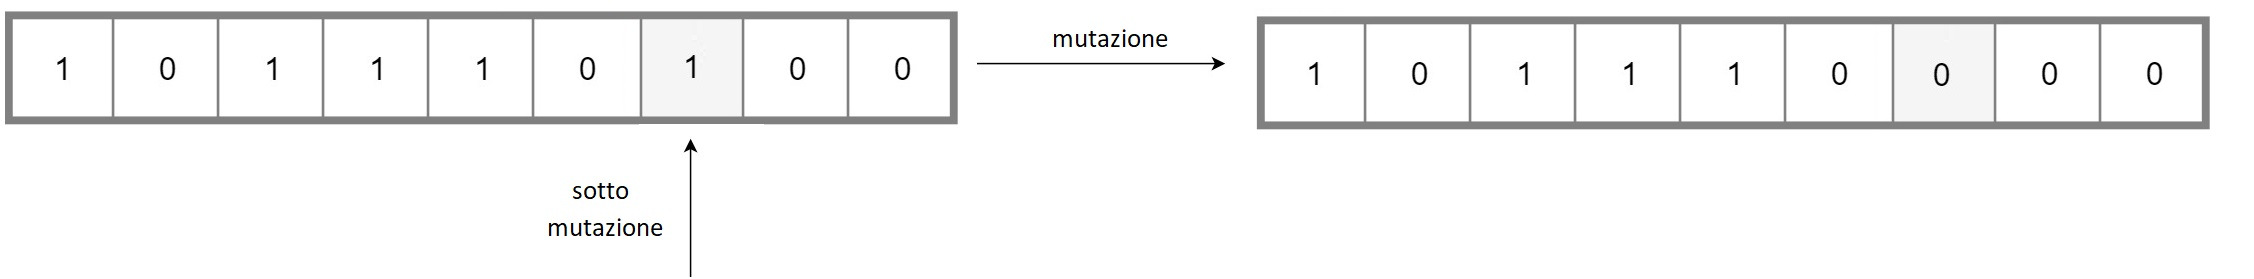
\includegraphics[scale=0.5]{Mutazione}

Figura 3: Esempio di mutazione
\end{center}


\vspace{2\baselineskip}
ALGORITMO GENETICO REALZIZZATO PER TSP
\vspace{2\baselineskip}

Gli \textit{AG} risolvono un determinato problema generando sempre nuove \textbf{popolazioni} di soluzioni dove in genere troviamo una fitness media piuttosto bassa, giungendo solamente dopo diverse generazioni a valori più elevati. Per poter applicare un algoritmo genetico, occorre anzitutto codificare numericamente le soluzioni e individuare una opportuna funzione di fitness. La codifica vettoriale dei cromosomi più adatta per i problemi di TSP risulta essere un vettore di interi dove ogni elemento identifica in maniera univoca una delle città da visitare mentre il suo posizionamento identifica l'ordine di visita.
La funzione di fitness realizzata riceve in ingresso una soluzione \textbf{ammissibile}\footnote{Per qualsiasi generazione non sono quindi accettabili elementi non validi per il problema in questione. La funzione XXXX LINK!!! è stata realizzata a a tale scopo.} e restituisce un valore reale pari al reciproco del suo costo PERCHE'?????? LO DICIAMO DOPO???????.
La prima generazione viene ottenuta attraverso il metodo \textbf{NearestNeightborGenetic} dell classe \textbf{Utility}. Come facilmente intuibile genera soluzioni che tendono a collegare nodi tra loro vicini, per maggiori dettagli si consulti l'apposita sezione ad esso dedicata nella appendice LINKK!!!!!!!!!!!!!!!!!.
La generazione di un \textit{figlio} a partire da due \textit{genitori} avviene attraverso il crossover ad un punto già presentato dove però solamente una delle due soluzioni ottenute entra a far parte del pool di candidati per la successiva generazione. Il crossover viene fornito dal metodo \textbf{GenerateChild}, sempre appartenente alla classe \textbf{Utility}, che viene descritto nell'apposito paragrafo LINK!!!!!!!, mentre i restanti condidati alla nuova generazione sono gli elementi stessi della generazione precedente (motivo?!?!?!).
Come operatore di selezione, si è deciso di utilizzare la \textit{selezione a roulette} dato che le soluzioni hanno lo stesso ordine di grandezza per quanto riguarda i loro costi QUI NON E' CHIARO CHE SIGNIFICA---INTENDI CHE LE FETTE CHE VENGONO FUORI NON SONO TROPPO DIVERSE??????. Infine la mutazione avviene con probabilità $p_{mutex}$ pari all'1\%.
Quanto descritto viene per la maggior parte gestito attraverso il metodo NOME!!!!!!!!!!!!! con l'ausilio della classe \textbf{pathgenetic}, procediamo quindi alla loro esposizione.

\vspace{2\baselineskip}
CLASSE PATHGENETIC
\vspace{2\baselineskip}

La classe \textbf{PathGenetic} utilizzata per memorizzare i dati di una soluzione generica, estende \textbf{PathStandard} già discussa nel paragrafo X.Y. aggiungendo due campi utili solamente per gli algoritmi genetici: il primo di tipo \textit{double} memorizza la fitness associata alla soluzione, il secondo di tipo intero identifica il circuito all'atto dell'estrazione dei percorsi che formeranno la generazione successiva\footnote{I suddetti parametri prendono nome \textbf{fittness} e \textbf{nRoulette}}.
La classe è dotata del metodo privato \textbf{CalculateFitness} il quale semplicemente setta la variabile fitness come descritto in precedenza:


\begin{lstlisting}

private void CalculateFitness()
{
     fitness = 1 / cost;
}

\end{lstlisting}

La variabile \textbf{cost} e l’array \textbf{path} sono ereditati da PathStandard e vengono settati utilizzando uno dei tre costruttori a disposizione

\begin{lstlisting}

public PathGenetic(int[] path, double cost) : base()
{
     this.path = path;
     this.cost = cost;
     CalculateFitness();
     nRoulette = -1;
}

public PathGenetic(int[] path, Instance inst) : base(path, inst)
{
    CalculateFitness();
    nRoulette = -1;
}

       
public PathGenetic(): base()
{
    fitness = -1;
    nRoulette = -1;
}

ANDREBBE UN COMMENTINO SU OGNUNO

\end{lstlisting}

\vspace{2\baselineskip}
FUNZIONE GENETICALGORITHM
\vspace{2\baselineskip}

Questa classe ha il compito di amministrare tutto tutte le fasi dell'algoritmo genetico. Per prima cosa si procede con una dichiariazione ed inizializzazione delle varie strutture dati necessarie. Tra queste troviamo due liste di \textit{PathGenetic} chiamate \textbf{OriginallyPopulated} e \textbf{ChildPoulation} che, durante tutto il processo, contengono rispettivamente l'insieme dei circuiti hamiltoniani che compongono la generazione $i-esima$ ed i figli da loro generati. La prima generazione viene ottenuta attraverso il metodo \textbf{NearestNeightborGenetic}, discusso in maggiore dettagli nella appendice LINK!!!!!, che, ricevendo la lista completa per ogni nodo di quali sono ad esso più vicini\footnote{Funzione già descritta qui LINK!!!!!!!!!!!!!!.}, costruisce le varie instanze tendendo a collegare i nodi più vicini tra loro\footnote{Il numero di componenti per ogni generazione viene chiesto in input all'utente e passato come parametro di ingresso alla funzione \textit{GeneticAlgorithm}.}.
Durante la generazione dei nuovi figli, poiché l'indice in cui è memorizzato un circuito all'interno di \textit{OriginallyPopulated}, dovuto in genere all'estrazione della rouellette, è casuale\footnote{Con casuale si intende che non è presente alcuna forma di correlazione fra l'indice e il costo della soluzione.} si è deciso di accoppiare circuiti memorizzati in celle adiacenti; la casualità di OriginallyPopulated consente di combinare fra loro soluzioni buone con altre meno buone e ciò statisticamente risulta particolarmente vantaggioso.
Una volta prodotti i figli è necessario procedere con la creazione della nuova generazione padre: questo viene eseguito dal metodo \textbf{NextPopulation} descritto in seguito. Per identificare il miglior circuito della generazione corrente si è realizzato il metodo \textbf{BestSolution}, qualora il valore ottenuto risulti minore dell’incumbent\footnote{Con incumbent si intende la miglio soluzione fin ora calcolata.} quest'ultimo viene aggiornato. L'algoritmo termina quanto scade il time limit fornito dall' utente.  Riportiamo di seguito il codice realizzato:

\begin{lstlisting}

PathGenetic incumbentSol = new PathGenetic();
PathGenetic currentBestPath = null;

List<PathGenetic> OriginallyPopulated = new List<PathGenetic>();
List<PathGenetic> ChildPoulation = new List<PathGenetic>();

List<int>[] listArray = Utility.BuildSLComplete(instance);

//Generate the first population
for (int i = 0; i < sizePopulation; i++)
OriginallyPopulated.Add(Utility.NearestNeightborGenetic(instance, rnd, true, listArray));
do
{
    //Generate the children
    for (int i = 0; i < sizePopulation; i++)
    {
        if (i % 2 != 0)
            ChildPoulation.Add(Utility.GenerateChild(instance, rnd, OriginallyPopulated[i], OriginallyPopulated[i - 1], listArray));
    }

    OriginallyPopulated = Utility.NextPopulation(instance, sizePopulation, OriginallyPopulated, ChildPoulation);

    //currentBestPath contains the best path of the current population
    currentBestPath = Utility.BestSolution(OriginallyPopulated, incumbentSol);

    if (currentBestPath.cost < incumbentSol.cost)
    {
        incumbentSol = (PathGenetic)currentBestPath.Clone();
        Utility.PrintGeneticSolution(instance, process, incumbentSol);
    }

    // We empty the list that contain the child
    ChildPoulation.RemoveRange(0, ChildPoulation.Count);

} while (clock.ElapsedMilliseconds / 1000.0 < instance.TimeLimit);

Console.WriteLine("Best distance found within the timelit is: " + incumbentSol.cost);

\end{lstlisting}


\vspace{2\baselineskip}
NEARESTNEIGHTBORGENETIC
\vspace{2\baselineskip}

Il corrente metodo è simile alla funzione NearestNeight discussa nel paragrafo X.Y ma con due differenze significative:

\begin{itemize}
    \item La sequenza degli elementi nell array che codifica il percorso creato dal metodo indicano l'ordine con cui il circuito visita i nodi. Si ricorda invece che il metodo NearestNeight produce percorsi codificati in array in cui alla generica posizione \textbf{i} è collocato il nodo successivo al nodo \textbf{i}. Tale modifica è dettata solamente da una agevolazione nell'utilizzo successivo di queste informazioni da parte dell'algoritmo genetico nella creazione della prima generazione.
    
    \item Poiché un algoritmo genetico è tanto migliore quanto gli individui che formano la popolazione di partenza hanno caratteristiche dissimili fra di loro, si è fatto in modo che i circuiti fossero il più possibili diversi gli uni dagli altri.
\end{itemize}


L' intestazione del metodo risulta essere:

\begin{lstlisting}

public static PathGenetic NearestNeightborGenetic(Instance instance, Random rnd, bool rndStartPoint, List<int>[] listArray)

\end{lstlisting}


Dove:


\begin{itemize}
    \item \textbf{instance}: oggetto della classe \textit{Instance} contenente tutti i dati che descrivono l'istanza del problema del Commesso Viaggiatore fornita in ingresso dall' utente;
    \item \textbf{rnd}: istanza della classe \textit{Random} precedentemente inizializzato con un seme random diverso per ogni iterazione del programma;
    \item \textbf{rndStartPoint}: variabile booleana che determina se il nodo di partenza sul quale viene applicato l' algoritmo nearest neightbor risulta essere casuale (in tal caso assume il valore true) oppure sia il nodo di default 0;
    \item \textbf{listArray}: lista in cui all'indice \textbf{i} è presente un vettore di dimensione instance.Nnodes al cui interno sono, in ordine crescente rispetto alla distanza assunta dal nodo \textbf{i}, presenti gli indici associati ai nodi del grafo.
\end{itemize}

Il circuito prodotto dal metodo viene memorizzato all'interno del vettore \textbf{heuristicSolution} avente una dimensione pari al numero di nodi del grafo. Poiché si vogliono soluzioni che siano il più possibile dissimili tra loro, è consigliabile fare in modo che \textit{rndStartPoint} sia posta a \textit{true}\footnote{Da notare che tale parametro non è settata runtime ma solamente via hardcode.}. Il vettore \textbf{VisitedNodes} di tipo bool è un vettore di supporto che memorizza all'indice \textbf{i} il valore logico true se il nodo \textbf{i} è già stato visitato, false altrimenti.

\begin{lstlisting}

 // heuristicSolution is the path of the current heuristic solution generate
    int[] heuristicSolution = new int[instance.NNodes];

    bool[] VisitedNodes = new bool[instance.NNodes];

    int firstNode = 0;

    //rndStartPoint define if the starting point is random or always the node 0 
    if (rndStartPoint)
        firstNode = rnd.Next(0, instance.NNodes);

    heuristicSolution[0] = firstNode;
    VisitedNodes[firstNode] = true;

\end{lstlisting}

Una volta definito il nodo di partenza i restanti nodi, che se visitati rispettando il loro ordine compongono un circuito hamiltoniano, son ottenuti attraverso un ciclo \textit{for}: alla generica iterazione \textbf{i} del ciclo, sfruttando la struttura dati listArray e la funzione \textbf{RndGenetic} si memorizza all'interno della variabile \textbf{nextNode} il nodo successivo visitato dal percorso sempre che questo sia ancora disponibile. Per verificarne la disponibilità si utilizza l'array \textit{VisitedNodes}, qualora non sia possibile utilizzare tale nodo si passa al successivo più vicino.


(la variabile contatore de ciclo for è inizializzata al valore 1, quindi il heuristicSolution[i-1] è memorizzato l' ultimo nodo visitato)  QUESTO VA COME COMMENTO NEL CODICE

\begin{lstlisting}

for (int i = 1; i < instance.NNodes; i++)
{
     bool found = false;
     int candPos = RndGenetic(rnd);
     int nextNode = listArray[heuristicSolution[i - 1]][candPos];
      do
      {
         //We control that the selected node has never been visited
          if (VisitedNodes[nextNode] == false)
          {
              VisitedNodes[nextNode] = true;
              heuristicSolution[i] = nextNode;
              found = true;
          }
          else
          {
              candPos++;
              if (candPos >= instance.NNodes - 1)
              {
                  nextNode = listArray[heuristicSolution[i - 1]][0];
                  candPos = 0;
              }
              else
                  nextNode = listArray[heuristicSolution[i - 1]][candPos];
          }

     } while (!found);
}

\end{lstlisting}


\vspace{2\baselineskip}
GENERATECHILD
\vspace{2\baselineskip}

Per generare un figlio si è realizzato il metodo \textbf{GenerateChild}, appartenente alla classe Utility, avente la seguente intestazione:

\begin{lstlisting}

public static PathGenetic GenerateChild(Instance instance, Random rnd, PathGenetic mother, PathGenetic father, List<int>[] listArray)

\end{lstlisting}

Dove:

\begin{itemize}
    \item \textbf{instance}: oggetto della classe Instance contenente tutti i dati che descrivono l'istanza del problema del Commesso Viaggiatore fornita in ingresso dall' utente;
    \item \textbf{rnd}: istanza della classe \textit{Random} precedentemente inizializzato con un seme random diverso per ogni iterazione del programma;
    \item \textbf{father}: circuito hamiltoniamo che sarà accopiato con il parametro mather;
    \item \textbf{mother}: hamiltoniamo che sarà accopiato con il parametro father;
    \item \textbf{listArray}: lista in cui all’ indice i è presente un vettore di dimensione instance.Nnodes al cui interno sono, in ordine crescente rispetto alla distanza assunta dal nodo i, presenti gli indici associati ai nodi del grafo.
\end{itemize}

Come precedentemente accennato il seguente metodo produce un figlio utilizzando l'operatore di crossover a singolo punto.

\begin{lstlisting}

int crossover = (rnd.Next(0, instance.NNodes));

for (int i = 0; i < instance.NNodes; i++)
{
   if (i > crossover)
      pathChild[i] = mother.path[i];
   else
      pathChild[i] = father.path[i];
}

\end{lstlisting}


Una volta creato il figlio, con una probabilità p = 0.01 viene effettuata su di esso una mutazione utilizzando il metodo \textbf{Mutation} LINK?!!?!?.


\begin{lstlisting}

if (rnd.Next(0, 101) == 100)
      Mutation(instance, rnd, pathChild);

\end{lstlisting}

Il figlio ottenuto quasi certamente non risulta essere un circuito ammissibile, per tale motivo si è progettato il metodo \textbf{Repair}. \'E interessante far notare che quest'ultimo non cerca di modificare i circuiti non modo da abbassarne il più possibile il costo ma al contrario è stato costruito in modo tale da risultare il più veloce possibile: soprattutto per popolazioni numerose e time limit alti tale scelta risulta essenziale. Di conseguenza i figli così prodotti sono tipicamente caratterizzati da un costo che con bassa probabilità risulta migliore rispetto a quello dei genitori e ciò comporta una saturazione dell'algoritmo dopo poche iterazioni (PERCHè?!?!?!?! METTERLO COME FOOTNOTE). Come operazione finale si è quindi deciso di applicare su di essi l'algoritmo \textbf{TwoOpt} ma solamente con una probabilità $p = 1 / (n/2)$, dove n è il numero dei nodi. La ragione per cui $p$ assume tale valore è dovuta al fatto che l'operazione di due ottimalità ha complessità computazionale O()[quando faccio il multistart controllo meglio quanto è la sua complessità] ed una sua applicazione più frequente rallenterebbe troppo l'algoritmo.

\begin{lstlisting}

if (ProbabilityTwoOpt(instance, rnd) == 1)
{
      child.path = InterfaceForTwoOpt(child.path);
      TSP.TwoOpt(instance, child);
      child.path = Reverse(child.path);
}

\end{lstlisting}

Da notare che la funzione per ottenere la due ottimalità è utilizzata da più metodi di risoluzione (multi-start ecc..) e necessita che il percorso della soluzione hamiltoniana sia memorizzato con un apposito formato diverso da quello presentato per l'algoritmo genetico: sono quindi necessarie due semplici interfacce \textbf{InterfaceForTwoOpt, Reverse}, i cui tempi di esecuzione sono $O(n)$.

\vspace{2\baselineskip}
NEXTPOPULATION
\vspace{2\baselineskip}

La funzione \textbf{NextPopulation}, appartenente alla classe \textbf{Utility}, consente di definire la nuova generazione scegliendone gli elementi tra la vecchia generazione ed i suoi figli attraverso una estrazione a roulette. La firma di tale funzione risulta essere:

\begin{lstlisting}

public static List<PathGenetic> NextPopulation(Instance instance, int sizePopulation, List<PathGenetic> FatherGeneration, List<PathGenetic> ChildGeneration)

\end{lstlisting}

Dove:

\begin{itemize}
    
    \item \textbf{instance}: oggetto della classe Instance contenente tutti i dati che descrivono l'istanza del problema del Commesso Viaggiatore fornita in ingresso dall' utente;
    \item \textbf{sizePopulation}: parametro che indica di quanti elementi deve essere la nuova generazione, per come è stato costruito il nostro programma questo parametro non varia mai ed è richiesto una sola volta all'utente;
    \item \textbf{FatherGeneration}: Lista contenente i circuiti che definiscono la generazione corrente;
    \item \textbf{ChildGeneration}: Lista contenente i circuiti figli generati da FatherGeneration utilizzando la funzione GenerateChild.

\end{itemize}

Per prima cosa uniamo le due liste di circuiti in quanto si è deciso che l'unico metro di giudizio durante la selezione deve essere il valore di fitness attribuito ad ogni soluzione indipendentemente dalla loro provenienza.

\begin{lstlisting}

for (int i = 0; i < ChildGeneration.Count; i++)
    FatherGeneration.Add(ChildGeneration[i]);

\end{lstlisting}

Passiamo ora a descrivere come è gestita la selezione a roulette, chiaramente esistono molteplici metodi e quello da noi scelto non ha alcun vantaggio significativo rispetto agli altri. L'idea alla base dell'algoritmo è di assegnare un valore univoco ad ogni circuito estraibile e di utilizzare tali valori molteplici volte come caselle della roulette, implementata come una lista di interi. Il numero di inserimenti per ogni valore è direttamente proporzionale alla fitness del circuito a cui è associato. Tutto questo viene per la maggior parte gestito all'interno del metodo \textbf{FillRoulette} LINK!!!!!!!!!!!!!!!!!, sempre definito nella classe \textbf{Utility}, che restituisce inoltre la grandezza della roulette così creata e poi memorizzato nella variabile \textbf{upperExtremity}:

\begin{lstlisting}

List<PathGenetic> nextGeneration = new List<PathGenetic>();
List<int> roulette = new List<int>();
Random rouletteValue = new Random();
int upperExtremity = FillRoulette(roulette, FatherGeneration);

\end{lstlisting}

La creazione della nuova generazione avviene estraendo valori random non superiori ad \textit{upperExtremity}, questi forniscono gli indici della lista-roulette le cui posizioni indicano indirettamente quale circuito deve far parte della nuova generazione. Naturalmente è possibile estrarre più volte la stessa soluzione, in questo caso la cosa va ignorata ripetendo nuovamente il processo. Nel complesso si dovranno estrarre (\textit{sizePopulation}) circuiti hamiltoniani.

\begin{lstlisting}

List<int> NumbersExtracted = new List<int>();
bool find = false;
int numberExtracted;

for (int i = 0; i < instance.SizePopulation; i++)
{
    do
    {
       find = true;
       numberExtracted = rouletteValue.Next(0, upperExtremity);
       //A path can't be extracted more than one time
       if (NumbersExtracted.Contains(roulette[numberExtracted]) == false)
       {
          find = false;
          NumbersExtracted.Add(roulette[numberExtracted]);
          nextGeneration.Add(FatherGeneration.Find(x => x.NRoulette == roulette[numberExtracted]));
       }
  } while (find);
}
return nextGeneration;

\end{lstlisting}

\vspace{2\baselineskip}
\textbf{APPENDICE}
\vspace{2\baselineskip}

\vspace{2\baselineskip}
FILL ROULETTE
\vspace{2\baselineskip}

Il metodo FillRoulette ha il compito di popolare la roulette in modo tale che la selezione sia proporzionale alla fitness. Associa ad ogni circuito un numero intero, chiamato \textbf{NRoulette}, progressivo e inserisce all'interno della roulette tale valore un numero di volte proporzionale al valore della fitness del circuito, infine ritorna la dimensione della roulette. La sua firma risulta essere:

\begin{lstlisting}

static int FillRoulette(List<int> roulette, List<PathGenetic> CurrentGeneration)

\end{lstlisting}

\begin{itemize}
    \item \textbf{roulette}: Lista di interi che rappresenta la roulette e che viene popolata dal metodo;
    \item \textbf{CurrentGeneration}: Lista contenente i circuiti candidati a far parte della nuova generazione;
\end{itemize}

Utilizzando il metodo \textbf{Estimate} LINK!!!!!!!!!!!!! si ottiene una costante intera che viene memorizzata all'interno della variabile \textbf{proportionalityConstant}: moltiplicare questo valore per la fitness di un circuito ci dice quante volte il corrispondente \textit{NRoulette} associato vada inserito nella ruolette. Poiché all'interno della stessa generazione i valori della fitness non variano per ordini di grandezza, tale costante viene per convenzione calcolata utilizzando il circuito memorizzato all'indice $0$ in \textit{CurrentGeneration}.
\begin{lstlisting}

int sizeRoulette = 0;
            
int proportionalityConstant = Estimate(CurrentGeneration[0].Fitness);

for (int i = 0; i < CurrentGeneration.Count; i++)
{
   int prob = (int)(CurrentGeneration[i].Fitness * proportionalityConstant);
   CurrentGeneration[i].NRoulette = i;
   sizeRoulette += prob;
   
   for (int j = 0; j < prob; j++)
     roulette.Add(i);
}
return sizeRoulette;


\end{lstlisting}

\vspace{2\baselineskip}
ESTIMATE
\vspace{2\baselineskip}

Il metodo Estimate genera una costante di proporzionalità in modo tale che, eseguendo il prodotto fra tale costante ed il valore ricevuto come parametro di ingresso, si ottenga una quantità sempre maggiore di 100 PERCHE'??????? A COSA SERVE?????. La sua firma risulta essere:

\begin{lstlisting}

static int Estimate(double sample)
{
    int k = 1;
    while (sample*k < 100)
    {
        k = k * 10;
    }
    return k;
}

\end{lstlisting}

Dove:

\begin{itemize}
    \item \textbf{sample}: Valore della fitness presa come campione.
\end{itemize}

\vspace{2\baselineskip}
REPAIR
\vspace{2\baselineskip}

Il metodo Repair è stato progettato per trasformare un percorso che non risulta essere un circuito hamiltoniano in un circuito hamiltoniano. Sappiamo che visitare più volte lo stesso nodo rende tale proprietà non vera così come la presenza di almeno un nodo isolato. L'algoritmo si sviluppa in due fasi: in un primo momento si eliminano dal vettore che codifica il percordo tutti i nodi duplicati, successivamente si fa in modo che quelli isolati vengano connessi al nodo ad essi più vicini. Un esempio di funzionamento dell'algoritmo è riportato nei tre grafici sottostanti.

\begin{center}
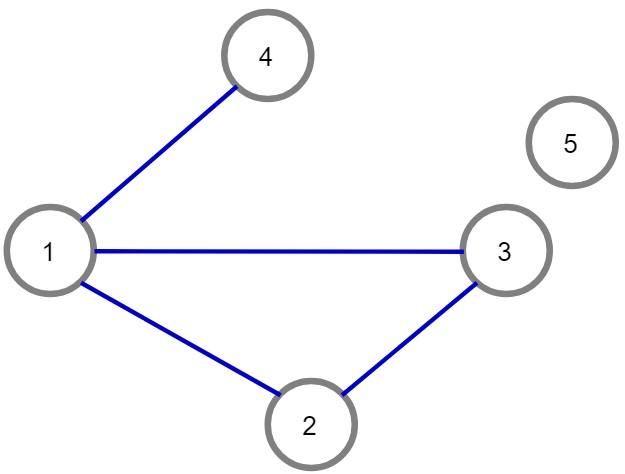
\includegraphics[scale=0.5]{circuitoF}

Figura 1: Circuito non hamiltoniano figlio
\end{center}

\begin{center}
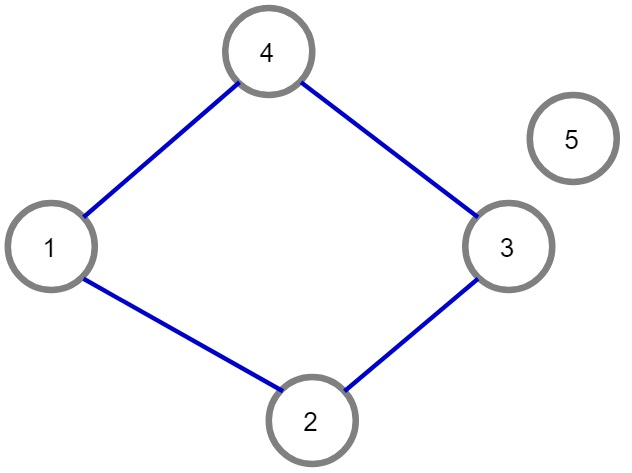
\includegraphics[scale=0.5]{circuitoH}  

Figura 2: Circuito hamiltoniano incompleto
\end{center}

\begin{center}
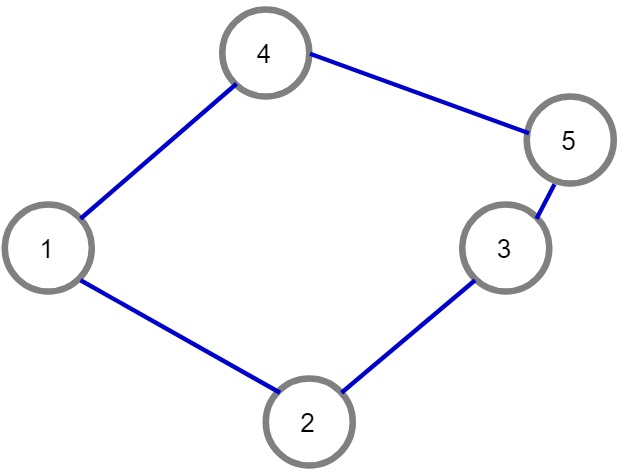
\includegraphics[scale=0.5]{circuitoC}

Figura 3: Circuito hamiltoniano figlio
\end{center}

Discutiamo ora il codice prodotto. Costruiamo due liste di interi chiamate \textbf{isolatedNodes} e \textbf{nearlestIsolatedNodes} dove rispettivamente contengono all'i-esimo elemento l'indice dell'i-esimo nodo isolato e l' indice del nodo ad esso più vicino\footnote{Ci sono in realtà delle eccezzioni a quest'ultima affermazione che vedremo in seguito}.
Per popolare tali liste utilizziamo i metodi \textbf{FindIsolatedNodes} LINK!!!!!! e \textbf{FindNearestNode} LINK!!!!!!!!!!.
Dichiariamo le due liste \textbf{pathIncomplete} e \textbf{pathComplete}, nella prima andiamo ad inserire il percorso originale privo degli elementi che lo rendono non hamiltoniano mentre nella seconda costruiamo il percorso completo di tutti i nodi ed hamiltoniano. Per ottenere quest'ultimo risultato procediamo ciclicamente con la copia di ogni elemento appartente a \textit{pathIncomplete} in \textbf{pathComplete} facendo però in modo che, se per un qualsisi $i, j, m$ vale $pathIncomplete[i]=nearlestIsolatedNodes[j]$, allora nel caso andiamo a porre $pathComplete[m]=pathIncomplete[i]$ dovrà anche valere $pathComplete[m+1]=isolatedNodes[j]$ e $pathComplete[m+2]=pathIncomplete[i+1]$ simili a quanto avviene nella Figura 3!!!!!!!!!!!!!!!!!!!!!!!.

\begin{lstlisting}

int positionInsertNode = 0;

for (int i = 0; i < pathIncomplete.Count; i++)
{
    if (nearlestIsolatedNodes.Contains(pathIncomplete[i]))
    {
        pathComplete[positionInsertNode] = pathIncomplete[i];
        pathComplete[positionInsertNode + 1] = isolatedNodes[nearlestIsolatedNodes.IndexOf(pathIncomplete[i])];
        positionInsertNode++;
    }
    else
        pathComplete[positionInsertNode] = pathIncomplete[i];

    positionInsertNode++;
}
return new PathGenetic(pathComplete, instance);
\end{lstlisting}

\vspace{2\baselineskip}
FINDISOLATEDNODES
\vspace{2\baselineskip}

Tale funzione viene utilizzata per identificare tutti i nodi isolati presenti in un generico percorso.
La sua firma risulta essere:

\begin{lstlisting}
static void FindIsolatedNodes(Instance instance, int[] path, List<int> isolatedNodes)
\end{lstlisting}

\begin{itemize}
    \item \textbf{instance}: oggetto della classe Instance contenente tutti i dati che descrivono l'istanza del problema del Commesso Viaggiatore fornita in ingresso dall' utente;
    \item \textbf{isolatedNodes}: Lista contenente gli indici di tutti i nodi isolati;
\end{itemize}

Data la semplicità del metodo non si ritiene utile far nessuna considerazione, riportiamo direttamente il codice realizzato.

\begin{lstlisting}

bool nodeIsVisited = false;

for (int i = 0; i < instance.NNodes; i++)
{
    for (int j = 0; j < instance.NNodes; j++)
    {
         if (pathChild[j] == i)
         {
            nodeIsVisited = true;
            //If the node is visited can exit to for
            break;
         }
    }

    //If the node has nevere been visited is a isolated noode
    if (nodeIsVisited == false)
       isolatedNodes.Add(i);

    //Configure nodeIsVisited to its default value
    nodeIsVisited = false;
}

\end{lstlisting}

\vspace{2\baselineskip}
FINDNEARESTNODE
\vspace{2\baselineskip}

Dato un certo circuito ed una lista di nodi isolati in esso contenuti, il metodo FindNearestNode fornisce per ognuno di essi il nodo più vicino \textit{valido} ossia che rispetti le seguenti condizioni:

\begin{itemize}
    \item  Non deve essere un nodo isolato;
    \item  Non deve essere il nodo più vicino di un nodo isolato precedentemente analizzato. In altre parole se $n_3$ è un nodo non isolato e risulta il nodo più vicino dei nodi isolati $n_1$ e $n_2$ non è possibile avere: $nearestNeighIsolNode[indice_{n_1}] = n_3 \wedge nearestNeighIsolNode[indice{n_2}] = n_3$. Per convenzione, supponendo $indice_{n_1} < indice_{n_2}$ vale $nearestNeighIsolNode[indice_{n_1}] = n_3$ mentre a $nearestNeighIsolNode[indice_{n_2}]$ viene assegnato il successivo nodo valido più vicino disponibile.
\end{itemize}

Il codice commentato della funzione viene riportato di seguito.

COMMENTA CODICE!!!!!!!!!!!!!!!!!!!!!!! RIPORTA TUTTO IL METODO!!!!!!!!!!!!!!!!! PUBLIC ...

\begin{lstlisting}

int nextNode = 0;
int nearestNode = 0;
bool find = true;

for (int i = 0; i < isolatedNodes.Count; i++)
{
    find = false;
    nextNode = 0;
    do
    {
       nearestNode = listArray[isolatedNodes[i]][nextNode];

       if (((isolatedNodes.Contains(nearestNode)) == false) && (nearestNeighIsolNode.Contains(nearestNode) == false))
       {
          nearestNeighIsolNode.Add(nearestNode);
          find = false;
       }
       else
       {
           nextNode++;
           find = true;
       }
    } while (find);
}

\end{lstlisting}

\vspace{2\baselineskip}
BESTSOLUTION
\vspace{2\baselineskip}

Il metodo BestSolution riceve come input una serie di percorsi hamiltoniani memorizzati attraverso la classe \textbf{PathGenetic} LINK!!!!!!!!!!!!!!!!!!!! ed in output fornisce quello a costo minore, la sua intestazione risulta essere:

\begin{lstlisting}

public static PathGenetic BestSolution(List<PathGenetic> population)

\end{lstlisting}

Dove:

\begin{itemize}
    \item \textbf{population}: Insieme di cammini hamiltoniani;
\end{itemize}

Di seguito il codice:

\begin{lstlisting}

PathGenetic currentBestPath = population[0];

for (int i = 1; i < population.Count; i++)
{
   if (population[i].cost < currentBestPath.cost)
      currentBestPath = population[i];
}

return currentBestPath;

\end{lstlisting}

\end{document}
